\documentclass[12pt, a4paper]{report}

\usepackage{listingsutf8}
\usepackage[utf8]{inputenc}
\usepackage[spanish]{babel}
\usepackage{amsfonts}
\usepackage{amsmath}
\usepackage{amssymb}
\usepackage{amsthm}
\usepackage{graphicx}
\usepackage{pdfpages}
\usepackage{spverbatim}
\usepackage{multirow}
\usepackage[left=3.5cm,right=1.5cm,top=2.5cm,bottom=2.5cm]{geometry}
\usepackage{xcolor}
\usepackage{textcomp}
\usepackage{listings}
\usepackage{hyperref}
\usepackage{floatrow}
\usepackage{wrapfig}
\author{Daniel Fernández Villanueva}
\title{\huge Sistema de monitorización inercial del movimiento de las extremidades superiores}

\makeatletter
\renewcommand*{\UTFviii@defined}[1]{%
  \ifx#1\relax
    \begingroup
      % Remove prefix "\u8:"
      \def\x##1:{}%
      % Extract Unicode char from command name
      % (utf8.def does not support surrogates)
      \edef\x{\expandafter\x\string#1}%
      \StringEncodingConvert\x\x{utf8}{utf16be}% convert to UTF-16BE
      % Hexadecimal representation
      \EdefEscapeHex\x\x
      % Enhanced error message
      \PackageError{inputenc}{Unicode\space char\space \string#1\space
                              (U+\x)\MessageBreak
                              not\space set\space up\space
                              for\space use\space with\space LaTeX}\@eha
    \endgroup
  \else\expandafter
    #1%
  \fi
}
\makeatother

\setcounter{tocdepth}{3}
\usepackage{color}
\definecolor{dkgreen}{rgb}{0,0.6,0}
\definecolor{gray}{rgb}{0.5,0.5,0.5}
\definecolor{mauve}{rgb}{0.58,0,0.82}
\definecolor{red}{rgb}{1.0, 0, 0}
\lstset{frame=tb,
  language=C++,
  aboveskip=3mm,
  belowskip=3mm,
  showstringspaces=false,
  columns=flexible,
  basicstyle={\small\ttfamily},
  numbers=left,
  frame=single,
  numberstyle=\tiny\color{gray},
  keywordstyle=\color{blue},
  commentstyle=\color{dkgreen},
  stringstyle=\color{mauve},
  breaklines=true,
  breakatwhitespace=true
  tabsize=4
}

\newtheorem{defn}{Definición}[section]

\begin{document}

\maketitle

\tableofcontents

\listoffigures

\listoftables

%%% ================ PARTE 1 : MEMORIA ================ %%%

\part{Memoria}

\pagestyle{headings}


%% ******** Capítulo 1 ******** %%

\chapter{ANTECEDENTES}


%% ******** Capítulo 2 ******** %%

\chapter{OBJETIVO DEL PROYECTO}

Este proyecto tiene como objetivo la implementación de un sistema de monitorización en tiempo real del movimiento de las extremidades superiores del cuerpo humano. En concreto, este sistema deberá ser capaz de registrar el estado de orientación principalmente de un brazo humano, aunque su uso será extensible a otros sistemas articulados. De forma inherente este objetivo, aparecen unos problemas a los que es necesario proporcionar una solución: 

\begin{enumerate}
\item \textbf{Toma de datos de los sensores}: \\
Realización de un sistema que permita obtener los datos que proporcionan los sensores utilizados para registrar el movimiento. Este sistema deberá de ser capaz de realizar la lectura en tiempo real, con mínima latencia y a una frecuencia aceptable. \\

\item \textbf{Tratamiento de los datos}: Una vez se tenga disponible un sistema para leer los datos de los sensores, el siguiente paso será procesar dichos datos para obtener las magnitudes necesarias para las distintas aplicaciones (Por ejemplo: orientación relativa entre sensores, ángulos de Euler, etc.)\\

\item \textbf{Utilización de los datos}: \\
En esta última fase se crearán los sistemas necesarios para la utilización de los datos con el objetivo deseado. En este proyecto se crearán tres aplicaciones concretas:

\begin{enumerate}

\item Visualización de un esquema del brazo en un visualizador 3D.

\item Control de un simulador de un brazo robótico.

\item Control del movimiento de un robot real.

\end{enumerate}

\end{enumerate}

En este documento se realizará una descripción detallada de las soluciones que se han adoptado para cada problema, y como se han incorporado dentro del sistema total de monitorización, de forma que cada parte se comunique con las demás de forma eficaz.

%%% ******** Capítulo 3 ******** %%%
\chapter{ESPECIFICACIONES DE DISEÑO}

En esta apartado se detallan las características esenciales que se pretenden implementar en el sistema de monitorización.

\begin{itemize}

\item \textbf{Flexibilidad}: que no sólo sea capaz de registrar la posición de un brazo humano, sino que sea aplicable a otro tipo de sistemas articulados, tanto humanos como de máquinas y robots. Por ello dicho sistema ha de ser flexible en cuanto a número de sensores y grados de libertad que se puedan monitorizar.

\item \textbf{Pequeño y ligero}: el sistema no puede ser demasiado aparatoso, ya que en se pretende colocarlo en extremidades humanas. Además no debería de dificultar la movilidad de la persona en absoluto.

\item \textbf{Fiabilidad}. Que sea lo más fidedigno posible en las medidas que proporciona. Esto puede tener mucha importancia en aplicaciones donde se requiera precisión.

\item \textbf{Económico}

\item \textbf{Versatilidad}. El sistema debería dejar la puerta abierta a poder ser incorporado en otras aplicaciones de forma sencilla, además de poder ser ampliado con mayor número de sensores o de distinto tipo sin mucho esfuerzo. 

\end{itemize}


%%% ******** Capítulo 4 ******** %%%
\chapter{DISEÑO DEL SISTEMA}

\section{Estudio de soluciones}

\subsection{Obtención del estado del brazo}

\subsubsection{Encoders}

\subsubsection{Sensores ópticos}

\subsubsection{Sensores inerciales}

Los sensores inerciales --normalmente incluidos dentro de una misma unidad llamada Unidad de Medición Inercial - Inertial Measurement Unit o IMU para abreviar-- utilizan un conjunto de acelerómetros, giróscopos y en ocasiones magnetómetros para la obtención de la velocidad, orientación, fuerzas magnéticas entre otros posibles parámetros. \\

Una de las principales desventajas que presentan los IMUs es la deriva que presentan a lo largo del tiempo. Esto es debido a que para obtener el estado en cierto tiempo, hacen uso de las medidas del estado anterior y los errores presentes se vas acumulando. Si embargo para la orientación es posible minimizar la deriva a un mínimo, incluso eliminarla, mediante un sistema llamado AHRS (\textit{Attitude and Heading Reference System}), en el que se utilizan la medida de la aceleración de la gravedad y el norte magnético para compensar las derivas que se obtienen con los giróscopos.

\subsubsection{Solución escogida: red de sensores inerciales xsens MTx}

Los sensores xsens MTx implementan la corrección AHRS para el cálculo de la orientación, por lo que proporcionan una medida de alta precisión y sin deriva apreciable de la orientación que presenta el sensor. Además es posible utilizar varios de estos sensores a la vez formando una red conectándolos a un máster xbus, lo que permitirá tomar los datos de los distintos eslabones que forman el brazo al mismo tiempo.

\begin{figure}[h]
	\centering
		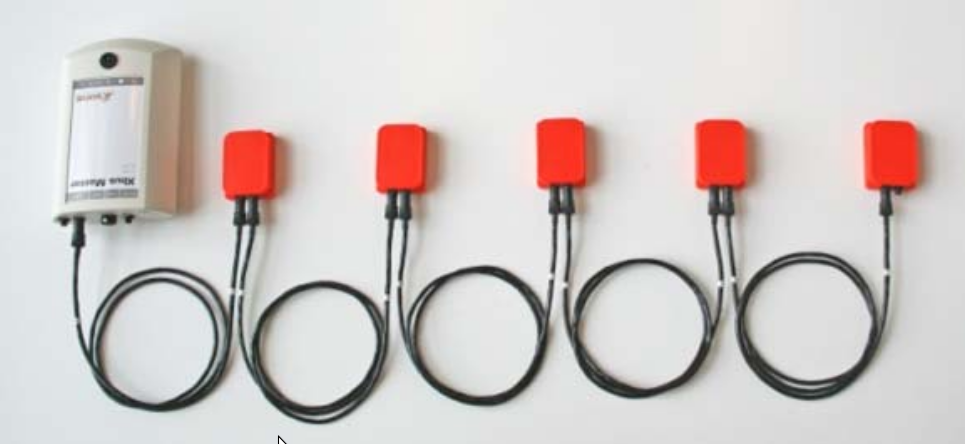
\includegraphics[scale=0.4]{../img/xbus_master.png} 
	\caption[Red de sensores xsens conectados a un máster xbus]{Red de sensores xsens conectados a un máster xbus.} 
	\label{fig: xbus_master}
\end{figure}

\subsection{Comunicación entre los sensores y el PC}

La conexión del máster Xbus al PC se realizará mediante cable USB. Para la toma de datos del sensor será necesario un programa especial llamado \textit{driver} que se encargue de gestionar las comunicaciones a través del puerto serie.

\subsubsection{Driver para la comunicación xbus Master - PC}

Las funcionalidades que se pretenden implementar en el \textit{driver} del Xsens son las siguientes:

\begin{itemize}

\item Capacidad de funcionar con varios sensores conectados

\item Posibilidad de realizar la configuración de los sensores.

\item Lectura a frecuencia aceptable.

\item Integración en el sistema ROS. Se verá más adelante la importancia de este punto.

\end{itemize}

Existen algunos drivers disponibles en internet preparados para trabajar en ROS con sensores Xsens. Sin embargo, lo que se han encontrado o bien sólo sirven para un sólo sensor, o trabajan en versiones bastante desfasadas de ROS y se encuentra poca o nula documentación sobre ellos. \\

La opción que se ha decidido seguir fue aprovechar que en la documentación de los sensores Xsens se proporcionan un conjunto de archivos con código en C++ para la comunicación a través del puerto serie con un sensor Xsens o un máster Xbus, y a partir de ellos construir el driver para la comunicación con los sensores y la publicación de los datos en ROS. Se realiza una descripción detallada de este programa en la sección \textit{Driver para la comunicación Xbus Master/Xsens - PC} del capítulo \textit{IMPLEMENTACIÓN DEL SOFTWARE}. 

\subsection{Comunicación entre programas}

Dada la multi-modularidad de la que se pretende dotar al sistema de monitorización, será necesario un sistema en el que distintos programas se puedan comunicar entre sí. Sería posible resolver las comunicaciones partiendo desde cero mediante sockets TCP/IP. Sin embargo es bastante más práctico utilizar algún tipo de plataforma que resuelva por ella misma las comunicaciones. En este proyecto se usará la plataforma ROS, que además de solucionar el tema de las comunicaciones, posee una gran cantidad de herramientas que van a ser de mucha utilidad. \\

\subsubsection{ROS}
\begin{wrapfigure}{r}{0.5\textwidth}
  \begin{center}
    
\includegraphics[scale=1.2]{../img/Logo-ROS.png} 
  \end{center}
  \caption[Logotipo de ROS]{Logotipo de ROS.}
  \label{fig: ros_logo}
\end{wrapfigure}
ROS (del inglés \textit{Robot Operating System} - Sistema Operativo Robótico) es una plataforma de desarrollo de software que incluye conjunto de utilidades centradas en ayudar al desarrollador en la creación de programas para el control de robots. Esta herramienta incorpora abstracción del hardware, drivers para dispositivos, librerías, visualizadores, utilidades para el intercambio de mensajes entre programas y administradores de paquetes de software, entre otras muchas cosas. ROS es además software abierto, bajo una licencia BSD, por lo que cualquier persona puede ver su código fuente y modificarlo.\\

\subsubsection{Herramientas proporcionadas por ROS}

La plataforma ROS proporciona solución a diversos problemas que vienen dados inherentemente al objetivo de este proyecto:

\begin{itemize}

\item \textbf{Creación y compilación de programas}: 

ROS proporciona librerías en los lenguajes C++, python y lisp en las que se implementan las diversas herramientas que pone a disposición, como intercambio de mensajes entre programas, servidor de parámetros, gestión del tiempo, entre muchas otras. En el presente proyecto se utilizará la implementación en C++ --\textbf{roscpp}--, que es la librería más apliamente difundida en la comunidad de ROS, además de estar diseñada para ser la librería más actualizada y con mayor número de herramientas.

Además ROS pone a disposición un gestor de paquetes de software con el fin de facilitar la reutilización de código. Un \textbf{paquete} es la forma más básica de organización del software en ROS. Un paquete puede contener programas --llamados \textbf{nodos}--, librerías, o cualquier otra cosa que posea cierta funcionalidad. La herramienta \textit{roscreate-pkg} permite la creación de un paquete de forma automática. 

En un \textbf{stack} de ROS se pueden incluir varios paquetes. Los \textit{stacks} tienen por fin hacer más sencillo compartir conjuntos de paquetes entre distintos ordenadores. Todos los paquetes creados en el presente proyecto se incluirán dentro de un mismo \textit{stack}.

\item \textbf{Comunicación entre programas:}
Uno de los puntos más fuertes de ROS son las herramientas que incluye para la comunicación entre programas, las cuales hacen posible crear un sistema totalmente distribuido, incluso entre varios ordenadores, en los que cada programa puede comunicarse con los demás mediante un interfaz sencilla y con mínima latencia. El sistema de intercomunicación de ROS se basa en los siguientes conceptos:

\begin{itemize}

\item \textbf{Máster}: El máster de ROS es el programa que se encarga de gestionar las comunicaciones entre los distintos nodos (programas de ROS). Permite que distintos nodos se encuentren entre si, lleva un registro de los \textit{publishers} y \textit{subscribers} de los distintos \textit{topics} y de los \textit{servicios}, además de proporcionar un \textit{servidor de parámetros}.

\item \textbf{Topics}: Los \textit{topics} son los canales de comunicación que utilizan los distintos \textit{nodos} para comunicarse entre sí. Esta comunicación es llevada a cabo mediante \textit{mensajes}. 

\item \textbf{Mensajes}: Un \textit{topic} acepta una determinada clase de mensaje. Los mensajes están compuestos por un conjunto de uno o varios tipos de datos --floats, strings, arrays, etc.--, o de otros mensajes en una estructura anidada. Existen unas definiciones de mensajes estándar, aunque es posible crear nuevas definiciones de estos mensajes. En este proyecto se han tratado de utilizar mensajes estándar en la medida de lo posible.

\item \textbf{Servicios}: Los \textit{topics} proporcionan una comunicación entre nodos de tipo publicador-subscriptor muy flexible, pero en ocasiones se requiere un sistema de tipo solicitud-respuesta, en el que un cliente envía un mensaje de solicitud y el servidor contesta con un mensaje de respuesta. Este tipo de comunicación se implementa en los \textit{servicios} de ROS. Los servicios están pensados para utilizarse en la solicitud de realización de ciertas tareas de vez en cuando. Para la comunicación de datos en \textit{streaming} --por ejemplo para el envío de los datos de los sensores-- es preferible el uso de \textit{topics}.

\item \textbf{Servidor de parámetros}: El servidor de parámetros de ROS es una especie de diccionario que puede ser accedido por los distintos nodos para crear, leer o modificar los valores de los parámetros almacenados en él. Se usará el servidor de parámetros para almacenar los valores de configuración de los sensores.

\item \textbf{Bags}: Los \textit{bags} de ROS son archivos que permiten almacenar los datos de uno o varios mensajes para su posterior reproducción. Permiten, por ejemplo, grabar los datos de los sensores para poder usarlos en otro momento o lugar en los que no estén disponibles los propios sensores.

\end{itemize}

\item \textbf{Visualización de datos}

\begin{itemize}

\item \textbf{rostopic}: El comando \textit{rostopic} permite conocer en tiempo real los topics que se encuentran publicados en ROS, y obtener los valores que se están publicando en ellos. Para obtener una lista de los topics se ejecutará el siguiente comando:

\begin{verbatim}
$ rostopic list
\end{verbatim}

Si se quisiera conocer los valors publicados se ejecutará el siguiente comando:

\begin{verbatim}
$ rostopic echo <nombre_del_mensaje>
\end{verbatim}

Por ejemplo, en la figura \ref{fig: rostopic_img} se muestran los datos de los acelerómetros de un sensor xsens conectado al PC. Es el resultado de ejecutar el siguiente comando:

\begin{verbatim}
$ rostopic echo /xsens_node/sensor0/acc
\end{verbatim}

\begin{figure}[h]
	\centering
		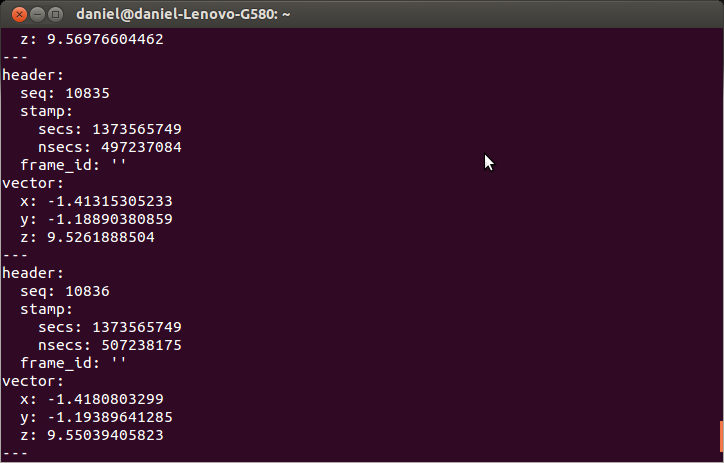
\includegraphics[scale=0.4]{../img/rostopic_img.png} 
	\caption[Comando rostopic mostrando datos de un sensor]{Comando rostopic mostrando datos de un sensor en tiempo real.} 
	\label{fig: rostopic_img}
\end{figure}

\item \textbf{rxplot}: La herramienta rxplot permite la representación gráfica de uno o varios valores a la vez, en tiempo real. Un ejemplo se muestra en la figura \ref{fig: rxplot_img}, que se ha obtenido con el comando:

\begin{verbatim}
$ rxplot -r 10 /xsens_node/sensor0/acc/vector/x:y:z
\end{verbatim}

\begin{figure}[h]
	\centering
		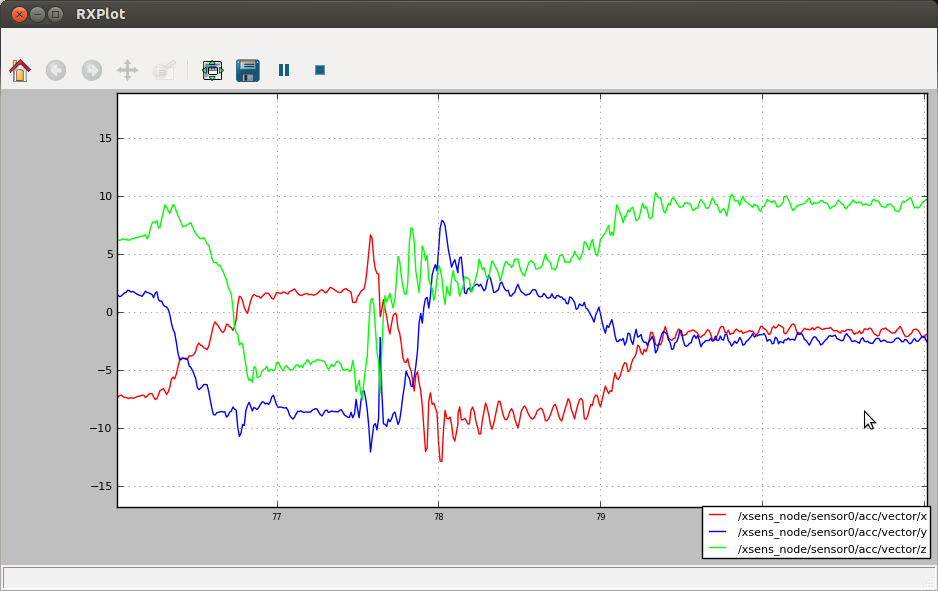
\includegraphics[scale=0.3]{../img/rxplot_img.png} 
	\caption[Programa rxplot mostrando datos de un sensor]{Programa rxplot mostrando una gráfica con los datos de los acelerómetros de un sensor en tiempo real} 
	\label{fig: rxplot_img}
\end{figure}

\end{itemize}

\item \textbf{Visualización 3D}

ROS incluye varios paquetes para la visualización y simulación 3D de objetos. Entre ellos, los más importantes son:

\begin{itemize}

\item \textbf{rviz}: El paquete rviz incluido en ROS es un paquete que permite la lectura de topics de ROS desde el propio programa, y asignar los valores a parámetros de la visualización. No es un simulador de física de objetos 3D, por lo que no permite la simulación de robots propiamente dicha.

\item \textbf{gazebo}: El programa Gazebo es un simulador de física de objetos rígidos. Permite la simulación de un robot o de un conjunto de robots, y su interacción entre ellos y con el ambiente. Además es posible obtener una simulación de la respuesta que tendrían ciertos tipos de sensores en el mundo real.  

\begin{figure}[h]
	\centering
		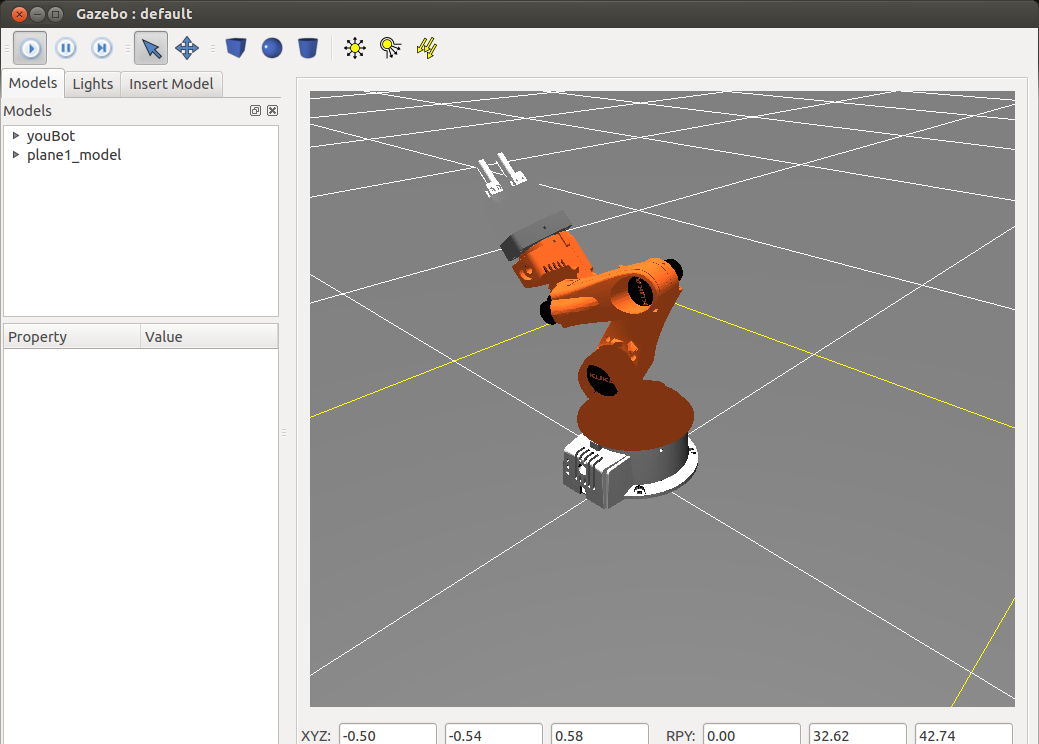
\includegraphics[scale=0.3]{../img/gazebo_img.png} 
	\caption[Programa Gazebo con la simulación del brazo del Youbot]{Programa Gazebo con la simulación del brazo del Youbot} 
	\label{fig: gazebo_img}
\end{figure}

En la documentación del robot YouBot viene incluída una simulación del brazo del robot en Gazebo con la que se puede interactuar mediante ciertos topics de ROS.

\end{itemize}

\end{itemize}

\subsection{Sistema operativo}

La plataforma ROS ha sido creada para trabajar principalmente en el sistema operativo Ubuntu. Existe otras versiones capaces de funcionar en otros sistemas operativos como Windows, pero son experimentales y no poseen todas las funcionalidades de la versión principal, además de carecer de soporte y ser algo inestables. Por ello, el sistema operativo elegido para la realización y ejecución del software será Ubuntu.

\subsubsection{El sistema operativo Ubuntu}

\begin{wrapfigure}{r}{0.5\textwidth}
  \begin{center}
    
\includegraphics[scale=0.3]{../img/ubuntu_logo.png} 
  \end{center}
  \caption[El sistema operativo Ubuntu]{El sistema operativo Ubuntu.}
  \label{fig: ubuntu_logo}
\end{wrapfigure}

Ubuntu es un sistema operativo con núcleo Linux, distribuído como software libre y de código abierto. Es la distribución más popular de los sistemas GNU/Linux en ordenadores personales.






\chapter{CÁLCULO DE LAS POSICIONES Y ORIENTACIONES DE LOS SENSORES}
\chaptermark{CÁLCULO DE LAS POSICIONES Y ORIENTACIONES}

Uno de los objetivos del proyecto es capturar el estado de orientación de los sensores para la utilizar los datos obtenidos en otros programas. Para ello es necesario utilizar un sistema de representación matemática de las orientaciones que permita la derivación de las magnitudes que se deseen (como ejes y ángulos de rotación) de forma rápida e inequívoca. En este capítulo se pretende dar una visión general de la derivación matemática y justificación de los algoritmos cuya implementación se mostrará en el capítulo \textit{IMPLEMENTACIÓN DEL SOFTWARE}.

\section{Formas de representar orientaciones espaciales}

Existen multitud de formas de representar la orientación de un sólido rígido:

\begin{itemize}

\item Ángulos de Euler
\item Eje y ángulo de Euler
\item Matriz de rotación
\item Cuaternión
\item Parámetros de Rodrigues
\item Parámetros de Cayley-Klein
\item \ldots

\end{itemize}

De todas estas formas de representación, los sensores xsens, al igual que muchos IMUs modernos, proporcionan la posibilidad de obtener los ángulos de Euler, la matriz de rotación y el cuaternión de rotación. En los siguientes apartados se analizarán las ventajas y desventajas de dichos sistemas y se escogerá la más conveniente.

\subsection{Ángulos de Euler}

Los ángulos de Euler son tres ángulos introducidos por Leonhard Euler para describir la orientación de un sólido rígido o de un sistema de referencia respecto a otro. Representan una secuencia de tres rotaciones elementales alrededor de los ejes de un sistema de coordenadas. Cualquier orientación puede describirse como la composición de tres rotaciones elementales, que pueden suceder alrededor de los ejes de un sistema de referencia fijo (rotaciones extrínsecas) o alrededor de los ejes de un sistema solidario al sólido rígido (rotaciones intrínsecas), lo que se denomina un sistema de referencia local. \\

Existen multitud de maneras distintas de expresar los ángulos de Euler, dependiendo del orden de los ejes sobre los cuales se realizan las rotaciones, y de si el sistema de referencia es local o global. La definición usada por los sensores xsens es la composición de rotaciones alrededor de los ejes XYZ en ese orden y un sistema de referencia global (fijo a la Tierra), en el que la ausencia de rotación equivale al vector Z paralelo a la línea que une la posición del sensor con el centro de la Tierra y sentido ascendente, y el vector X en dirección al norte magnético. \\

Los ángulos proporcionados por el sensor son:

\begin{itemize}

\item $\phi$ = \textit{roll} = rotación alrededor del eje X $[-\frac{\pi}{2}, \frac{\pi}{2}]$

\item $\theta$ = \textit{pitch} = rotación alrededor del eje Y $[-\frac{\pi}{4}, \frac{\pi}{4}]$

\item $\psi$ = \textit{yaw} = rotación alrededor del eje Z $[-\frac{\pi}{2}, \frac{\pi}{2}]$

\end{itemize}

El uso de ángulos de Euler presenta un par de problemas:

\begin{itemize}

\item Si $\theta$ se extiende al intervalo $[-\frac{\pi}{2}, \frac{\pi}{2}]$ en vez de restringirse a $[-\frac{\pi}{4}, \frac{\pi}{4}]$, la descripción de la rotación no es única. En este caso existen dos posibles soluciones para cada orientación, por lo que los datos que proporciona el sensor no son suficientes para diferenciar entre un estado de rotación u otro.

\item Cuando $\theta$ se acerca al valor $\pm\frac{\pi}{4}$ existe una singularidad matemática causada por la infinitud de valores que pueden adquirir $\phi$ y $\psi$ en dicho caso. Esta situación es la que se conoce con el nombre de \textit{gimbal lock}.

\end{itemize}

Estos problemas no están presentes en los demás modos de salida del sensor.

\subsection{Matriz de rotación}

Una matriz de rotación es una matriz usada para expresar una rotación en un espacio euclideo. Si se supone un sistema generador $S$ con un conjunto de vectores base $B$ del espacio vectorial $V$:

$$ B = \{\vec{i}, \vec{j}, \vec{k}\}, \quad \vec{i} = \begin{bmatrix} 1\\0\\0 \end{bmatrix} \quad  \vec{j} = \begin{bmatrix} 0\\1\\0 \end{bmatrix} \quad  \vec{k} = \begin{bmatrix} 0\\0\\1 \end{bmatrix} $$
$$ V = S(\vec{i}, \vec{j}, \vec{k}) $$

Se somete al sistema de coordenadas a una rotación $R$. Los vectores base sufren una transformación que se puede expresar con respecto al sistema de referencia original de la siguiente forma:

$$ \vec{i}' = \alpha_{11}\vec{i} + \alpha_{21}\vec{j} + \alpha_{31}\vec{k} = \begin{bmatrix}  \alpha_{11}\\\alpha_{21}\\\alpha_{31} \end{bmatrix} $$
$$ \vec{j}' = \alpha_{12}\vec{i} + \alpha_{22}\vec{j} + \alpha_{32}\vec{k} = \begin{bmatrix} \alpha_{12}\\\alpha_{22}\\\alpha_{32} \end{bmatrix} $$
$$ \vec{k}' = \alpha_{13}\vec{i} + \alpha_{23}\vec{j} + \alpha_{33}\vec{k} = \begin{bmatrix} \alpha_{13}\\\alpha_{23}\\\alpha_{33} \end{bmatrix} $$

donde $\alpha_{ij}$ son las componentes de la base rotada expresadas con respecto a la base original. Se tiene un vector cualquiera en la base original:

$$ \vec{v} = a\vec{i} + b\vec{j} + c\vec{k} = \begin{bmatrix} a\\b\\c \end{bmatrix} $$

Tras la rotación las componentes del vector expresadas conforme a la nueva base no variarán debido a que se mueve solidario al sistema de referencia. Por lo tanto el vector rotado es el siguiente:

$$ \vec{v}' = a\vec{i}' + b\vec{j}' + c\vec{k}' $$

Sustituyendo los vectores $\vec{i}'$, $\vec{j}'$, $\vec{k}'$ por sus expresiones respecto a la base original:

$$ \vec{v}' = a \begin{bmatrix}  \alpha_{11}\\\alpha_{21}\\\alpha_{31} \end{bmatrix} + b \begin{bmatrix}  \alpha_{12}\\\alpha_{22}\\\alpha_{32} \end{bmatrix}  + c \begin{bmatrix}  \alpha_{13}\\\alpha_{23}\\\alpha_{33} \end{bmatrix} = \begin{bmatrix}  a\alpha_{11} + b\alpha_{12} + c\alpha_{13} \\ a\alpha_{21} + b\alpha_{22} + c\alpha_{23}\\ a\alpha_{31} + b\alpha_{32} + c\alpha_{33} \end{bmatrix} $$

Este nuevo vector puede expresarse como el producto de una matriz por un vector:

$$ \vec{v}' = \begin{bmatrix}  \alpha_{11} & \alpha_{12} & \alpha_{13} \\ \alpha_{21} & \alpha_{22} & \alpha_{23}\\ \alpha_{31} & \alpha_{32} & \alpha_{33} \end{bmatrix} \begin{bmatrix} a \\ b \\ c \end{bmatrix} = R \vec{v}$$

Dicha matriz $R$ es la denominada matriz de rotación. Se comprueba que puede interpretarse como una matriz cuyos elementos son las componentes de los vectores base del sistema de coordenadas rotado expresados con respecto al sistema de coordenadas original.\\

El uso de matrices de rotación evita los problemas que presentan los ángulos de Euler; Proporcionan una descripción biunívoca del estado de rotación del sensor, y además no presentan el problema del \textit{gimbal lock}. 

\subsection{Cuaternión}

Los cuaterniones son una extensión de los números complejos ideada por el matemático irlandés William Rowand Hamilton con el objetivo de poder utilizar el análisis complejo en un espacio de 3 dimensiones.Un cuaternión es la combinación lineal de cuatro cantidades \{$1$, $i$, $j$, $k$\}, donde cada una de las cantidades \{$i$, $j$, $k$\} es la raíz cuadrada de $-1$, de tal forma que se cumplen las siguientes propiedades:

$$ i^2 = j^2 = k^2 = ijk = -1 $$

La expresión general de un cuaternión es la siguiente:

\begin{equation} \label{eq: gen_quaternion}
q = w + xi + yj + zk
\end{equation}

donde $w$, $x$, $y$ y $z$ son números reales. Los cuaterniones satisfacen las leyes conmutativa y asociativa de la suma, la ley asociativa de la multiplicación, las leyes distributivas de la multiplicación respecto a la suma y la existencia de los elementos neutros para la suma y la multiplicación. Una propiedad importante de los cuaterniones es que no satisfacen la propiedad conmutativa de la multiplicación.

\begin{table}[h]
\center
\begin{tabular}{|l|c|}

\hline
\multicolumn{2}{|c|}{\textbf{Propiedades de los cuaterniones}}\\
\hline
Conmutativa respecto a la suma & $ q_1 + q_2 = q_2 + q_1 $ \\
\hline
Asociativa respecto a la suma & $ q_1 + (q_2 + q_3) = (q_1 + q_2) + q_3 $ \\
\hline
Asociativa respecto a la multiplicación & $ q_1(q_2q_3) = (q_1q_2)q_3 $ \\
\hline
\multirow{2}{*}{Distributiva de la multiplicación respecto a la suma} & $ q_1(q_2 + q_3) = q_1q_2 + q_1q_3 $ \\
\cline{2-2}
 & $ (q_1 + q_2)q_3 = q_1q_3 + q_2q_3 $ \\
\hline
Elemento neutro de la suma & $ q + 0 = q $ \\
\hline
Elemento neutro de la multiplicación & $ q1 = 1q = q $ \\
\hline
No conmutatividad de la multiplicación & $q_1q_2 \not= q_2q_1$\\
\hline
\end{tabular}

\caption{Propiedades de los cuaterniones}
\label{tab:propiedades_cuaterniones}

\end{table}

Los cuaterniones presentan las mismas ventajas que las matrices de rotación en cuanto a unicidad y ausencia de \textit{gimbal lock}. Pero además son superiores a las matrices en los siguientes aspectos:

\begin{itemize}

\item Su representación en memoria es más compacta que la de las matrices (4 números frente a 9 necesarios para la matriz).

\item Se puede construir fácilmente un cuaternión a partir de un eje y un ángulo, y viceversa. Estas operaciones son más complejas para matrices de rotación y ángulos de Euler.

\item Mayor estabilidad numérica de los cuaterniones. Tras la composición de varias rotaciones en un ordenador necesariamente se van a acumular errores de redondeo. Para que los cuaterniones y matrices representen una rotación deben ciertas propiedades. En concreto, los cuaterniones tienen que ser unitarios y la matriz de rotación tiene que ser ortogonal. Es bastante más fácil normalizar un cuaternión para que vuelva a representar una rotación que recomponer una matriz para que vuelva a ser ortogonal.

\item Además con los cuaterniones es sencillo componer una interpolación esférica (llamada \textit{slerp - spherical linear interpolation} ) para producir una rotación suave a lo largo del tiempo.

\end{itemize}

\subsection{Solución elegida: cuaterniones}

Por la gran cantidad de ventajas que presentan los cuaterniones con respecto a las demás formas de representar una rotación, éstos serán los escogidos para registrar el estado de orientación de los sensores y realizar los cálculos matemáticos.

\section{Utilización de cuaterniones para la representación de rotaciones de un sólido rígido}

En esta sección se verá cómo describir rotaciones simples y composiciones de rotaciones de un sólido rígido mediante el uso de cuaterniones. \\

Sea un vector unitario:

\begin{equation}
\vec{e} = e_x i + e_y j + e_z k, \quad \|e\| = \sqrt{e_x^2 + e_y^2 + e_z^2} = 1
\end{equation}


Se definirá el cuaternión de rotación con ángulo $\theta$ sobre el eje definido por el vector $\vec{e}$:

\begin{equation}
q(\theta, \vec{e}) = \cos \left(\frac{\theta}{2}\right) + \sin \left(\frac{\theta}{2}\right) e_x i + \sin \left(\frac{\theta}{2}\right) e_y j + \sin \left(\frac{\theta}{2}\right) e_z k 
\end{equation}

Este cuaternión representa la orientación de un sólido tras sufrir una rotación de ángulo $\theta$ alrededor del eje definido por el vector $\vec{e}$. Se puede descomponer el cuaternión como suma de un número real y un cuaternión imaginario puro unitario multiplicado por otro número real:

\begin{equation}
q( \theta , \vec{e}) = \cos \left(\frac{\theta}{2}\right) + \sin \left(\frac{\theta}{2}\right) e  
\end{equation}

Donde $e$ es el cuaternión imaginario puro (parte real nula) cuyas componentes se corresponden a las del vector unitario $\vec{e}$ que define el eje de rotación. \\

Por cuestión de comodidad definimos las siguientes variables:

\begin{equation}
c_i = \cos \left( \frac{\theta_i}{2} \right)
\end{equation}
\begin{equation}
s_i = \sin \left( \frac{\theta_i}{2} \right)
\end{equation}

De tal forma que ahora el cuaternión se escribirá de la siguiente manera:

\begin{equation} \label{eq: q_theta_e}
q(\theta_i, \vec{e_i}) = c_i + s_i e_i
\end{equation}

Si se tienen en cuenta las propiedades del cuadro \ref{tab:propiedades_cuaterniones}, el producto de dos cuaterniones se puede expresar de esta forma:

\begin{equation} \label{eq: E11}
q_1 q_2 = \left( c_1 + s_1 e_1 \right) \left( c_2 + s_2 e_2 \right) = c_1 c_2 + c_1 s_2 e_2 + c_2 s_1 e_1 + s_1 s_2 e_1 e_2
\end{equation}

En donde:

\begin{multline} \label{eq: E10}
e_1 e_2 = (e_{1_x} i + e_{1_y} j + e_{1_z} k)(e_{2_x} i + e_{2_y} j + e_{2_z} k) = \\
= e_{1_x} i (e_{2_x} i + e_{2_y} j + e_{2_z} k) + e_{1_y} j (e_{2_x} i + e_{2_y} j + e_{2_z} k) + e_{1_z} k (e_{2_x} i + e_{2_y} j + e_{2_z} k) = \\
= -(e_{1_x} e_{2_x} + e_{1_y} e_{2_y} + e_{1_z} e_{2_z}) + i (e_{1_y} e_{2_z} + e_{1_z} e_{2_y}) + j (-e_{1_x} e_{2_z} + e_{1_z} e_{2_x}) + k (e_{1_x} e_{2_y} + e_{1_y} e_{2_x}) \\
\end{multline}

Se definirán las siguientes operaciones con cuaterniones imaginarios puros (parte real nula):

\begin{defn}
Sean dos cuaterniones imaginarios puros $q_1$ y $q_2$ tales que:
$$ q_1 = x_1i + y_1j + z_1k $$
$$ q_2 = x_2i + y_2j + z_2k $$
Se define el operador producto escalar ($\cdot$) como:
$$ q_1 \cdot q_2 = x_1x_2 + y_1y_2 + z_1z_2 $$
Este operador presenta las mismas propiedades que el mismo operador para vectores de 3 dimensiones:
$$ q_1 \cdot q_2 = q_2 \cdot q_1 $$
$$ q_1 \cdot q_1 = \|q_1\|^2 $$
$$ q_1 \cdot q_2 = 0 \iff q_1 \perp q_2 $$
\end{defn}

\begin{defn}
Sean dos cuaterniones imaginarios puros $q_1$ y $q_2$ tales que:
$$ q_1 = x_1i + y_1j + z_1k $$
$$ q_2 = x_2i + y_2j + z_2k $$
Se define el operador producto vectorial ($\times$) como:
$$ q_1 \times q_2 = \begin{bmatrix} 
i & j & k \\
x_1 & y_1 & z_1 \\
x_2 & y_2 & z_2
\end{bmatrix} = (y_1z_2 - z_1y_2)i + (z_1x_2 - x_1z_2)j + (x_1y_2 - y_1x_2)k$$
Este operador presenta las mismas propiedades que el mismo operador para vectores de 3 dimensiones:
$$ q_1 \times q_2 = - (q_2 \times q_1) $$
$$ q_1 \times q_2 = 0 \iff q_1 \parallel q_2 $$
$$ q_1 \times q_2 = q_3 : q_3 \perp q_1 \wedge q_3 \perp q_2 $$
\end{defn}

Utilizando la definición de estos operadores se puede simplificar la ecuación \eqref{eq: E10}:

\begin{equation} \label{eq: e_1e_2}
e_1 e_2 =  -e_1 \cdot e_2 + e_1 \times e_2
\end{equation}

Por lo tanto, sustituyendo \eqref{eq: e_1e_2} en la ecuación \eqref{eq: E11}:

$$ q_1 q_2 = c_1 c_2 + c_1 s_2 e_2 + c_2 s_1 e_1 + s_1 s_2 (-e_1 \cdot e_2 + e_1 \times e_2) $$

\begin{equation}
q_1 q_2 = c_1 c_2 - s_1 s_2 (e_1 \cdot e_2) + c_1 s_2 e_2 + c_2 s_1 e_1 + s_1 s_2 (e_1 \times e_2)
\end{equation}

\begin{defn}
El conjugado de un cuaternión $ q = c + s e $ se define como el cuaternión resultado de negar la parte imaginaria. Se representará de la siguiente manera:

\begin{equation} \label{eq: E17}
conj(q) = q^* = c - s e
\end{equation}
\end{defn}

\begin{defn}
La norma o magnitud de un cuaternión $ q = w + xi + yj + zk $ se define como la siguiente operación:

\begin{equation} \label{eq: E16}
\|q\| = \sqrt{w^2 + x^2 + y^2 + z^2}
\end{equation}
\end{defn}

Esta magnitud representaría una hipotética longitud que tendría el cuaternión si el espacio de los cuaterniones $\mathbb{H}$ se identifica con un espacio euclídeo $\mathbb{R}^4$. Para un cuaternión de rotación se tiene que:

$$ q = c + se, \quad \|q\| = \sqrt{c^2 + \|se\|^2} = \sqrt{c^2 + s^2} = 1 $$

Dado a que se va a trabajar siempre con cuaterniones unitarios (también llamados \textit{versores}), se podrá asumir lo siguiente:

\begin{equation}
\|q\| = 1 , \quad q^{-1} = \frac{q^*}{\|q\|^2} = q^*
\end{equation}

De tal forma que:

\begin{equation} \label{eq: qq*}
qq^* = q^*q = 1
\end{equation}

\subsection{Rotación de un vector alrededor de un eje y un ángulo dados}

Se puede realizar la rotación de un vector $\vec{p}$ alrededor de un eje $\vec{e}$ y un ángulo $\theta$ mediante la siguiente operación:

\begin{equation} \label{eq: E14}
p' = qpq^*, \quad q = q(\theta, \vec{e})
\end{equation}

donde $p$ es el cuaternión asociado al vector $\vec{p}$, que se define como:

\begin{equation} \label{eq: E15}
\vec{p} = p_x\vec{i} + p_y\vec{j} + p_z\vec{k} \quad \Rightarrow \quad p = p_xi + p_yj + p_zk
\end{equation}

\begin{figure}[h] 
	\centering
		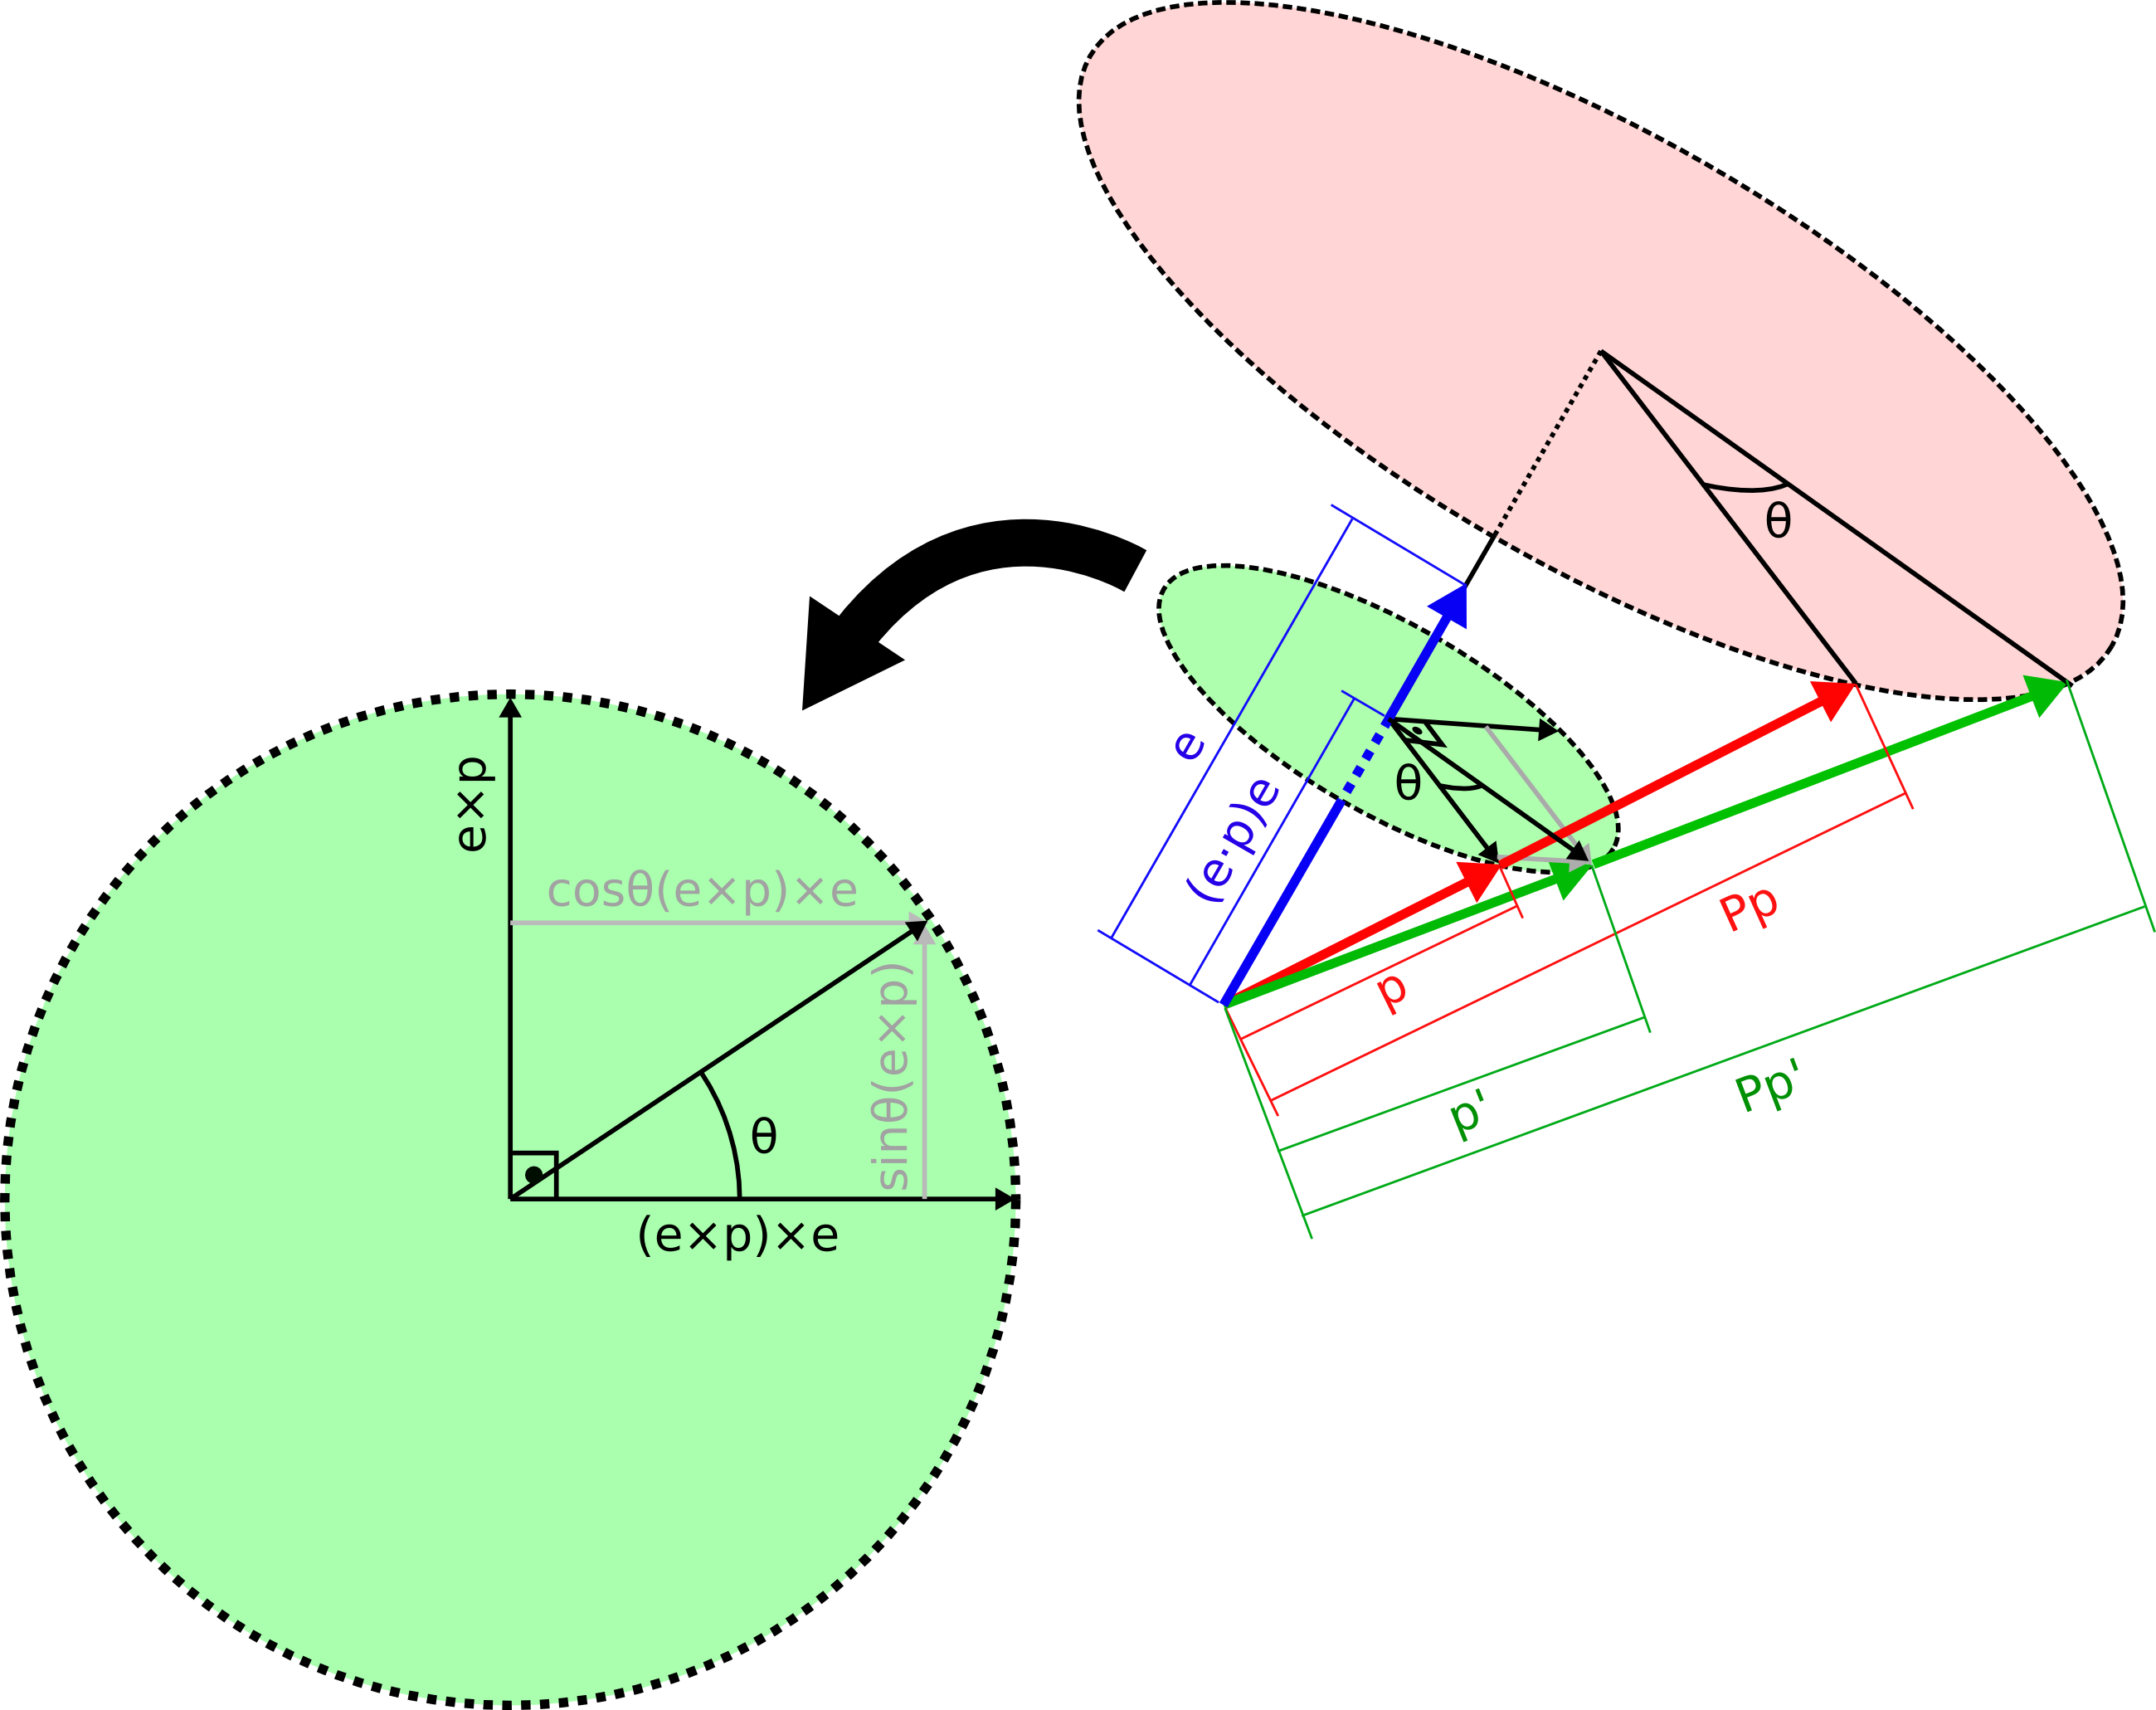
\includegraphics[scale=1.1]{../img/rotation_quaternion.png} 
	\caption{Rotación de un vector mediante la operación $q_1pq_1^*$}
	\label{fig: rot_cuat}
\end{figure}

Se comprueba que en efecto la ecuación \eqref{eq: E14} es cierta. Desarrollando la expresión para un cuaternión genérico $q$ y un vector expresado como cuaternión $Pp$, donde $P$ es el módulo del vector y $p$ es el cuaternión asociado al vector normalizado:

$$ q(Pp)q^* = P(qpq^*) = P(c+se)p(c-se) = P(cp + sep)(c - se) = P(c^2p - cspe + csep - s^2epe) $$

Se aplican las propiedades de los cuaterniones unitarios vistas anteriormente:

\begin{equation} \label{eq: E12} 
q(Pp)q^* = P(c^2p + 2cs(e \times p) + s^2(e \cdot p)e - s^2(e \times p) \times e) 
\end{equation}

Se le puede asignar a cada término un significado geométrico:

\begin{itemize}

\item $(e \cdot p)e$ es la proyección de $p$ sobre $e$
\item $(e \times p)$ es un vector perpendicular a $e$ y a $p$. Formaría una supuesta coordenada $y$ en el círculo de giro.
\item $(e \times p) \times e$ es un vector perpendicular al anterior, cuyo origen podemos situar al final de $(e \cdot p)e$ y su final, en el mismo punto que $p$. Sería la coordenada $x$ del círculo de giro.

\end{itemize}  

En la figura \ref{fig: rot_cuat} se muestra más claramente el significado de cada término.\\

Es posible descomponer así el término $c^2p$ como suma de dos de estos vectores:

$$ c^2p = c^2(e \cdot p)e + c^2(e \times p) \times e $$

Sustituyendo el resultado en \eqref{eq: E12}:

$$ q(Pp)q^* = P\left(c^2(e \cdot p)e + c^2(e \times p) \times e + 2cs(e \times p) + s^2(e \cdot p)e - s^2(e \times p) \times e)\right) $$

Reorganizando términos:

$$ q(Pp)q^* = P\left((c^2 + s^2)(e \cdot p)e + (c^2 - s^2)(e \times p) \times e + 2cs(e \times p)\right) $$

Si se aplican igualdades trigonométricas a esta expresión, teniendo en cuenta que $c = \cos\left(\frac{\theta}{2}\right)$ y $s = \sin\left(\frac{\theta}{2}\right)$:

$$ q(Pp)q^* = P\left((e \cdot p)e + \cos\theta(e \times p) \times e + \sin\theta(e \times p)\right) $$

De la figura \ref{fig: rot_cuat} se deduce que $ p' = (e \cdot p)e + \cos\theta(e \times p) \times e + \sin\theta(e \times p)$, y por lo tanto se puede concluir que:

$$ q(Pp)q* = Pp' $$

Por lo que para un vector cualquiera $\vec{v}$ se cumple que $qvq^* = v'$, donde $v'$ es el cuaternión asociado al vector rotado. \\

Si se realiza una multiplicación a la izquierda por $q_1^*$ y por la derecha por $q_1$ a cada término de la ecuación \eqref{eq: E14} (lo que equivale a realizar una rotación dada por el cuaternión $q_1^*$):

\begin{equation}
q_1^*p'q_1 = q_1^*(q_1pq_1)q_1^*
\end{equation}

\begin{equation}
q_1^*p'q_1 = p
\end{equation}

se obtiene el punto inicial, de lo que se deduce que el conjugado del cuaternión representa una rotación inversa a la del cuaternión original:

\begin{equation}
q = q\left(\theta, \vec{e} \right) \quad \Rightarrow \quad q^* = q\left(\theta, -\vec{e} \right) = q\left(-\theta, \vec{e}\right)
\end{equation}

\subsection{Composición de rotaciones en coordenadas extrínsecas}

El cuaternión de rotación definido por $q\left(\theta, \vec{e}\right)$ representa una rotación alrededor de un eje $\vec{e}$ fijo al sistema de referencia global.\\

Realizando una nueva rotación a un vector que ha sufrido una rotación definida por $q_1 = q\left(\theta_1, \vec{e_1}\right)$, se obtendrá una rotación compuesta por una primera rotación seguida de otra rotación caracterizada por $q_2 = q\left(\theta_2, \vec{e_2} \right)$:

$$ \text{ Primera rotación: } \quad p' = q_1pq_1^*, \quad q_1 = q(\theta_1, \vec{e_1}) $$
$$ \text{ Segunda rotación: }\quad p'' = q_2p'q_2^*, \quad q_2 = q(\theta_2, \vec{e_2}) $$

\begin{equation}
p'' = q_2(q_1pq_1^*)q_2^* = (q_2q_1)p(q_1^*q_2^*) = q_{12}pq_{12}^*
\end{equation}

Se puede expresar la composición de dos rotaciones como un nuevo cuaternión que resulta de la multiplicación en orden inverso de los cuaterniones que definen las dos rotaciones:

\begin{equation}
q_{12} = q_2 q_1
\end{equation}

De aquí se deduce que el conjugado del producto de dos cuaterniones es el producto de los conjugados en orden inverso:

\begin{equation}
q_{12} = \left(q_2q_1\right)^* = q_1^*q_2^*
\end{equation}

De forma análoga, para $n$ cuaterniones:

\begin{equation}
q_{12 \dotsc (n-1)n} = q_nq_{n-1} \dotsm q_2q_1
\end{equation}

\begin{equation}
\left( q_{12 \dotsc (n-1)n} \right)^* = \left( q_nq_{n-1} \dotsm q_2q_1 \right)^* = q_1^*q_2^* \dotsm q_{n-1}^*q_n^*
\end{equation}

\subsection{Composición de rotaciones en coordenadas intrínsecas}

Para representar una rotación alrededor de un eje expresado en el sistema de referencia local del sólido, se tendrá que realizar la construcción del cuaternión teniendo en cuenta que dicho eje ha sufrido la misma rotación que el sólido con respecto al sistema de referencia global. Supongamos un sólido que ha sufrido una rotación inicial representada por el cuaternión $q_1$. Se quiere realizar una rotación de ángulo $\theta_2$ sobre un eje $e_2^L$ en coordenadas locales. Dicho eje expresado en coordenadas globales será:

$$ e_2^G = q_1e_2^Lq_1^* $$

Teniendo en cuenta la ecuación \eqref{eq: q_theta_e}, el cuaternión de rotación asociado al ángulo $\theta_2$ y el vector local $e_2^L$ despueś de que el sólido haya sufrido una rotación definida por el cuaternión $q_1$ será:

$$ q_{2_{q_1}} = q(\theta_2, \vec{e_2}^G) = \cos\left( \frac{\theta_2}{2}\right) + \sin\left( \frac{\theta_2}{2} \right)e_2^G $$

\begin{equation} \label{eq: q_2_q_1}
q_{2_{q_1}} =  c_2 + s_2(q_1e_2^Lq_1^*)
\end{equation} 

\subsection{Relación entre rotaciones intrínsecas y extrínsecas}

El algoritmo de obtención de los ángulos de Euler que se explicará más adelante proporciona una solución en el caso de ejes solidarios al sensor, esto es, en un sistema de coordenadas intrínsecas. Es posible obtener con este algoritmo soluciones en un sistema extrínseco que pueden ser de utilidad en ciertas aplicaciones. A continuación se demostrará que una rotación compuesta por varias rotaciones en el sistema de coordenadas intrínseco del sólido rígido se corresponde a la composición de rotaciones en el sistema extrínseco realizadas en orden inverso.\\

Se define un cuaternión de rotación asociado al eje local $\vec{e_2}^L$ después de haber sufrido una rotación definida por el cuaternión $q_1 = q\left( \theta_1 , \vec{e_1} \right)$ como:

\begin{equation}
q_{2_{q_1}} = q\left(\theta_2 , \vec{e_2}^L \right) , \quad \vec{e_2}^L = (q_1e_2q_1^*)_{\vec{v}}
\end{equation}

Se va a suponer sin pérdida de generalidad que la primera rotación se ha realizado desde una posición en la que coinciden los sistemas local y global  \footnote{Por definición el origen del  cuaternión de orientación ($q = 1$) del sensor es la orientación donde coinciden el sistema global y local. Por ello, el eje de rotación en los dos sistemas coincidirá y por lo tanto el cuaternión de rotación será el mismo.}, por lo que:

\begin{equation}
q_1^G = q_1^L = q_1
\end{equation}

donde $q_1^G$ es la rotación alrededor de un eje en coordenadas globales y $q_1^L$ la rotación en coordenadas locales.\\

Para demostrar la afirmación de partida se tendrá que demostrar la veracidad de la siguiente igualdad:

\begin{equation}
q_2^Lq_1 = q_1q_2^G
\end{equation}

Se reordenará la igualdad para que los cálculos sean más sencillos:

\begin{equation} \label{eq: E01}
q_2^Lq_1 = q_1q_2^G \iff q_2^L = q_1q_2^Gq_1^*
\end{equation}

Desarrollo del lado izquierdo de la igualdad:

\begin{equation} \label{eq: q_2I}
q_2^L = c_2 + s_2(q_1e_2q_1^*)
\end{equation}

\begin{multline} \label{eq: q_1e_2q_1}
q_1e_2q_1^* = (c_1 + s_1e_1)e_2(c_1 - s_1e_1) = (c_1e_2 + s_1e_1e_2)(c_1 - s_1e_1) = \\
= c_1^2e_2 + s_1c_1e_1e_2 - c_1s_1e_2e_1 - s_1^2e_1e_2e_1 = c_1^2e_2 + s_1c_1(e_1e_2 - e_2e_1) - s_1^2e_1e_2e_1
\end{multline}

De \eqref{eq: e_1e_2} se tiene lo siguiente:

$$ e_1e_2 = -e_1 \cdot e_2 + e_1 \times e_2 $$
$$ e_2e_1 = -e_2 \cdot e_1 + e_2 \times e_1 = -e_1 \cdot e_2 - e_1 \times e_2 $$

\begin{equation} \label{eq: e_1e_2e_2e_1}
e_1 e_2 - e_2 e_1 = 2(e_1 \times e_2)
\end{equation}

$$ e_1 e_2 e_1 = (-e_1 \cdot e_2 + e_1 \times e_2)e_1 =(-e_1 \cdot e_2)e_1 + (e_1 \times e_2)e_1 $$

De esta ecuación:

$$ (e_1 \times e_2)e_1 = -(e_1 \times e_2) \cdot e_1 + (e_1 \times e_2) \times e_1 $$

$(e_1 \times e_2)$ será un vector perpendicular a $e_1$, por lo que $(e_1 \times e_2) \cdot e_1 = 0$:

$$ (e_1 \times e_2)e_1 = (e_1 \times e_2) \times e_1 $$

Por lo tanto:

\begin{equation} \label{eq: e_1e_2e_1}
e_1 e_2 e_1 = -(e_1 \cdot e_2)e_1 + (e_1 \times e_2) \times e_1
\end{equation}

Sustituyendo en \eqref{eq: q_1e_2q_1}:

$$ q_1e_2q_1^* = c_1^2e_2 + s_1c_1(e_1e_2 - e_2e_1) - s_1^2e_1e_2e_1 = $$
$$ c_1^2e_2 + 2s_1c_1(e_1 \times e_2) - s_1^2(-(e_1 \cdot e_2)e_1 + (e_1 \times e_2) \times e_1) $$

\begin{equation}
q_1e_2q_1^* = c_1^2e_2 + 2s_1c_1(e_1 \times e_2) + s_1^2(e_1 \cdot e_2)e_1 - s_1^2(e_1 \times e_2) \times e_1
\end{equation}

Finalmente, sustituyendo en \eqref{eq: q_2I}:

$$ q_2^L = c_2 + s_2(c_1^2e_2 + 2s_1c_1(e_1 \times e_2) + s_1^2(e_1 \cdot e_2)e_1 - s_1^2(e_1 \times e_2) \times e_1) $$

\begin{equation} \label{eq: E02}
q_2^L = c_2 + s_2c_1^2e_2 + 2s_1s_2c_1(e_1 \times e_2) + s_1^2s_2(e_1 \cdot e_2)e_1 - s_1^2s_2(e_1 \times e_2) \times e_1
\end{equation}

Ahora se procederá a desarrollar el lado derecho de la igualdad \eqref{eq: E01}:

$$ q_1q_2^Gq_1^* = (c_1 + s_1 e_1)(c_2 + s_2 e_2)(c_1 - s_1 e_1) = $$

$$ = (c_1c_2 + s_2c_1e_2 + s_1c_2e_1 + s_1s_2e_1e_2)(c_1 - s_1 e_1) = $$

$$ = c_1^2c_2 + s_2c_1^2e_2 + s_1c_1c_2e_1 + s_1s_2c_1e_1e_2 - s_1c_1c_2e_1 - s_1s_2c_1e_2e_1 - s_1^2c_2e_1e_1 - s_1^2s_2e_1e_2e_1 $$

Como $\|e_1\| = 1$, se tendrá que:

\begin{equation}
e_1e_1 = -e_1 \cdot e_1 + e_1 \times e_1 = -1
\end{equation}

Sustituyendo y reorganizando:

$$ q_1q_2^Gq_1^* = c_2 + s_2c_1^2e_2 + s_1s_2c_1(e_1e_2 - e_2e_1) - s_1^2s_2e_1e_2e_1 $$

De \eqref{eq: e_1e_2e_2e_1} y \eqref{eq: e_1e_2e_1}:

$$ q_1q_2^Gq_1^* = c_2 + s_2c_1^2e_2 + 2s_1s_2c_1(e_1 \times e_2) - s_1^2s_2(-(e_1 \cdot e_2)e_1 + (e_1 \times e_2) \times e_1) $$

\begin{equation} \label{eq: E03}
q_1q_2^Gq_1^* = c_2 + s_2c_1^2e_2 + 2s_1s_2c_1(e_1 \times e_2) + s_1^2s_2(e_1 \cdot e_2)e_1 - s_1^2s_2(e_1 \times e_2) \times e_1
\end{equation}

Finalmente se compara \eqref{eq: E02} con \eqref{eq: E03}:

$$ q_2^L = c_2 + s_2c_1^2e_2 + 2s_1s_2c_1(e_1 \times e_2) + s_1^2s_2(e_1 \cdot e_2)e_1 - s_1^2s_2(e_1 \times e_2) \times e_1 $$

$$ q_1q_2^Gq_1^* = c_2 + s_2c_1^2e_2 + 2s_1s_2c_1(e_1 \times e_2) + s_1^2s_2(e_1 \cdot e_2)e_1 - s_1^2s_2(e_1 \times e_2) \times e_1 $$

Se puede ver que los términos a la derecha de la igualdad son exactamente los mismos, por lo que se tiene que:

\begin{equation} \label{eq: q2I}
q_2^L = q_1q_2^Gq_1^*
\end{equation}

Y por lo tanto es verdad la afirmación de partida. Una rotación $q_2^L$ alrededor de un eje local tras una rotación $q_1$ es la misma que la rotación global $q_2^G$ seguida de la rotación $q_1$:

\begin{equation} \label{eq: q2lq1}
q_2^Lq_1 = q_1q_2^G
\end{equation}

Ahora se va a suponer que el cuaternión $q_1$ está compuesto de otras dos rotaciones, que se van a expresar de forma global y local según la ecuación \eqref{eq: q2lq1}:

$$ q1 = q_{1b}^Lq_{1a} = q_{1a}q_{1b}^G $$

Sustituyendo en \eqref{eq: q2lq1}:

$$ q_2^Lq_{1b}^Lq_{1a} = q_{1a}q_{1b}^Gq_2^G $$

Renombrando los términos:

$$ q_3^Lq_{2}^Lq_{1} = q_{1}q_{2}^Gq_3^G $$

Aplicando el mismo método de forma sucesiva se puede generalizar el resultado a $n$ rotaciones:

\begin{equation}
q_n^L \dotsm q_3^Lq_{2}^Lq_{1} = q_{1}q_{2}^Gq_3^G \dotsm q_n^G
\end{equation}

Se concluye que la composición de $n$ rotaciones en coordenadas locales es la misma que la composición de $n$ rotaciones en coordenadas globales realizadas en orden inverso.

\subsection{Orientación relativa entre dos sólidos}

Se tienen dos sólidos con sendos sistemas de coordenadas $S_1$ y $S_2$. Definiremos la rotación relativa del sólido $1$ sobre el sólido $2$ como la rotación existente entre sus sistemas de coordenadas.\\

\begin{center}
\begin{figure}[h]
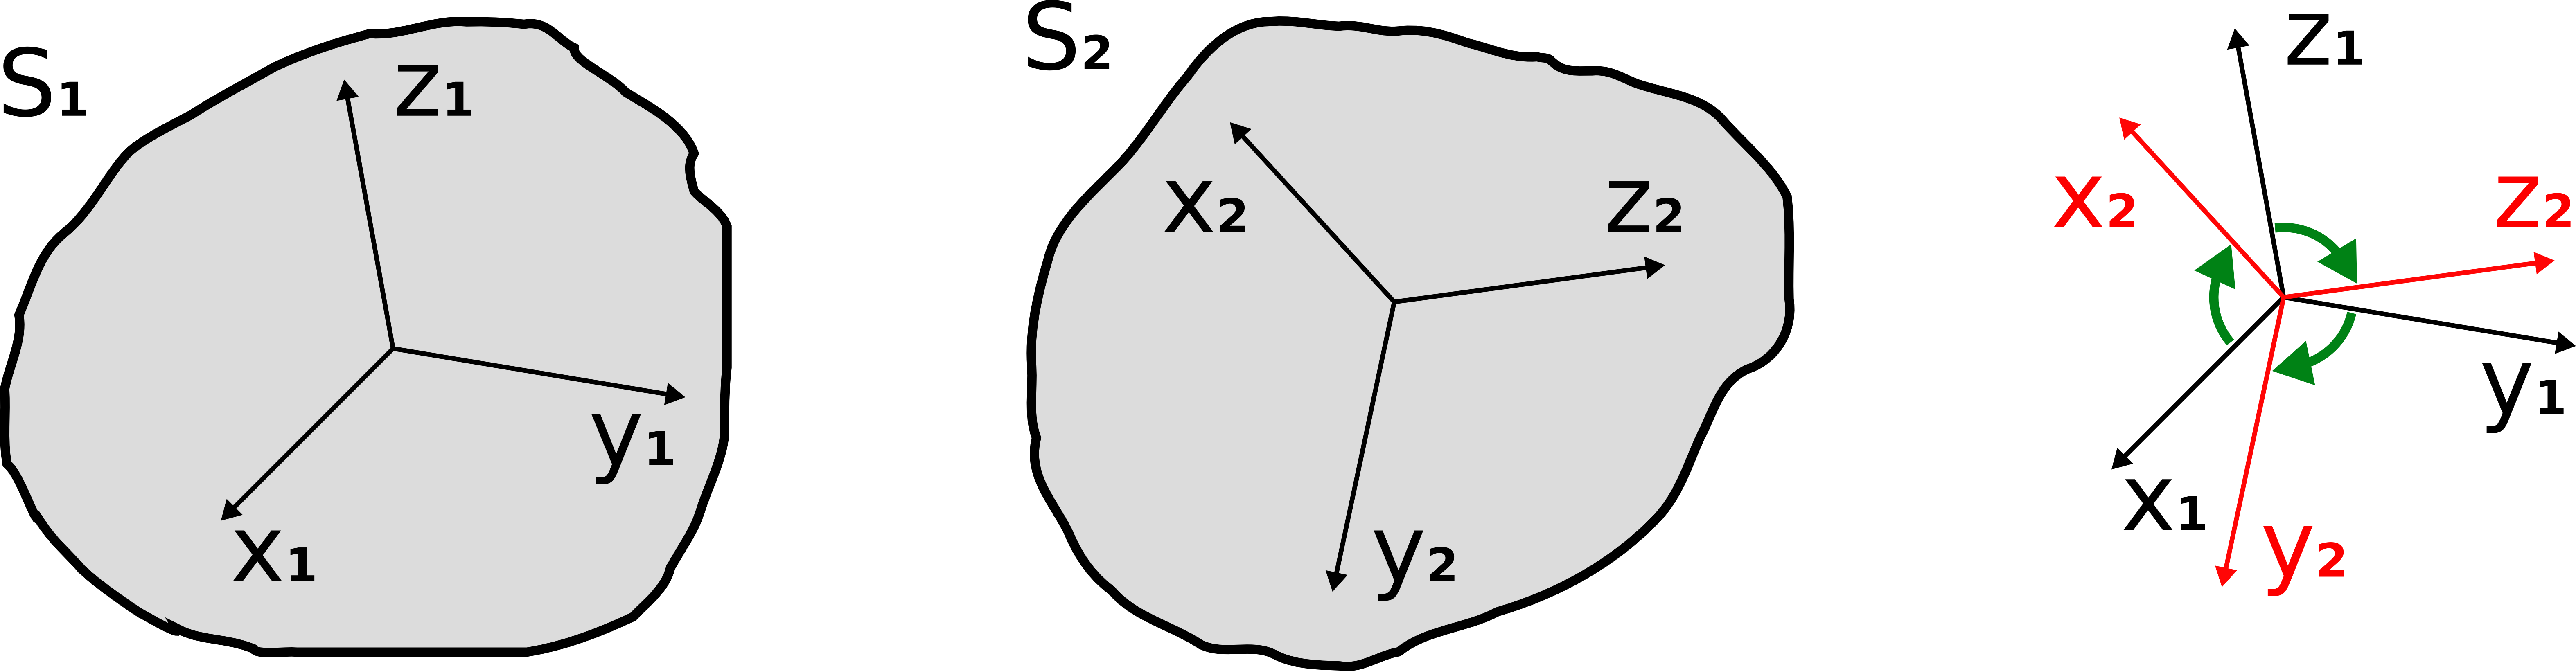
\includegraphics[scale=1]{../img/relative_orientation.png} 
\caption{Orientación relativa entre dos sólidos rígidos}
\end{figure}
\end{center}

Otra forma de verlo es que la rotación relativa es la rotación que tendría el sólido $2$ si el sistema de coordenadas del sólido $1$ fuera el global. De esta forma se podrá calcular el cuaternión que define la orientación relativa entre los dos sólidos aplicando una rotación a ambos de forma que el sistema de coordenadas del sólido $1$ coincida con el global. Se llamará $q_1$ al cuaternión que define la orientación del sólido $1$ y $q_2$ al que define la orientación del sólido $q_2$. Si se aplica una rotación $q_1^*$ a ambos, esto es, una rotación inversa a la del sólido $1$, se obtiene lo siguiente:

$$ \text{Sólido 1: } q_1' = q_1^*q_1 = 1 $$
$$ \text{Sólido 2: } q_2' = q_1^*q_2 = q_{S_2S_1} $$

donde $q_{S_2S_1}$ es la orientación relativa del sólido 2 con respecto al sólido 1. Generalizando este resultado se obtiene una expresión general para hallar la rotación relativa de un sólido $A$ con respecto a un sólido $B$:

\begin{equation} \label{eq: E18}
q_{S_AS_B} = q_B^*q_A
\end{equation}

Esta expresión tiene interés a lo hora del cálculo de los ángulos de Euler en la articulación de un brazo articulado si se conocen los cuaterniones de rotación globales de los dos eslabones que forman la articulación.

\section{Cálculo de la posición del brazo}

Una vez sean conocidas las orientaciones de los sensores, sabiendo que dichos sensores se encuentran solidarios al brazo y cuyo eje $x$ se ha orientado en sentido longitudinal de acuerdo a la figura \ref{fig: posiciones_brazo}, resulta muy sencillo obtener las posiciones de cada punto del brazo sabiendo su posición inicial. \\

Un brazo articulado simple se definirá por un conjunto de 3 longitudes $\{L_1, L_2, L_3\}$ que representan las distancias hombro-codo, codo-muñeca y muñeca-punta de dedo respectivamente, y por 3 cuaterniones $\{q_1, q_2, q_3\}$ que indican el estado de orintación de brazo, antebrazo y mano repectivamente. Dado que para los sensores xsens la posición inicial es aquella en la que su eje $x$ apunta al norte magnético, y el eje $z$ es vertical hacia arriba, se establecerá como posición inicial del brazo aquella en la que el eje longitudinal de todos los eslabones apunta hacia el norte magnético. En esta posición se cumple que:

$$ q_1 = q_2 = q_3 = 1 $$

Además como el eje $x$ se corresponde con el elemento base $i$, los puntos iniciales de hombro, codo, muñeca y punta de dedo son:

$$ p_0^i = 0 \quad p_1^i = L_1i \quad p_2^i = p_1^i + L_2i = (L_1 + L_2)i \quad p_3^i = p_2^i + L_3i = (L_1 + L_2 + L_3)i $$

Se tomará como origen de coordenadas global la posición del hombro $p_0$. Cada eslabón tendrá por origen de coordenadas local la articulación inmediatamente anterior.

\begin{figure}[h] 
	\centering
		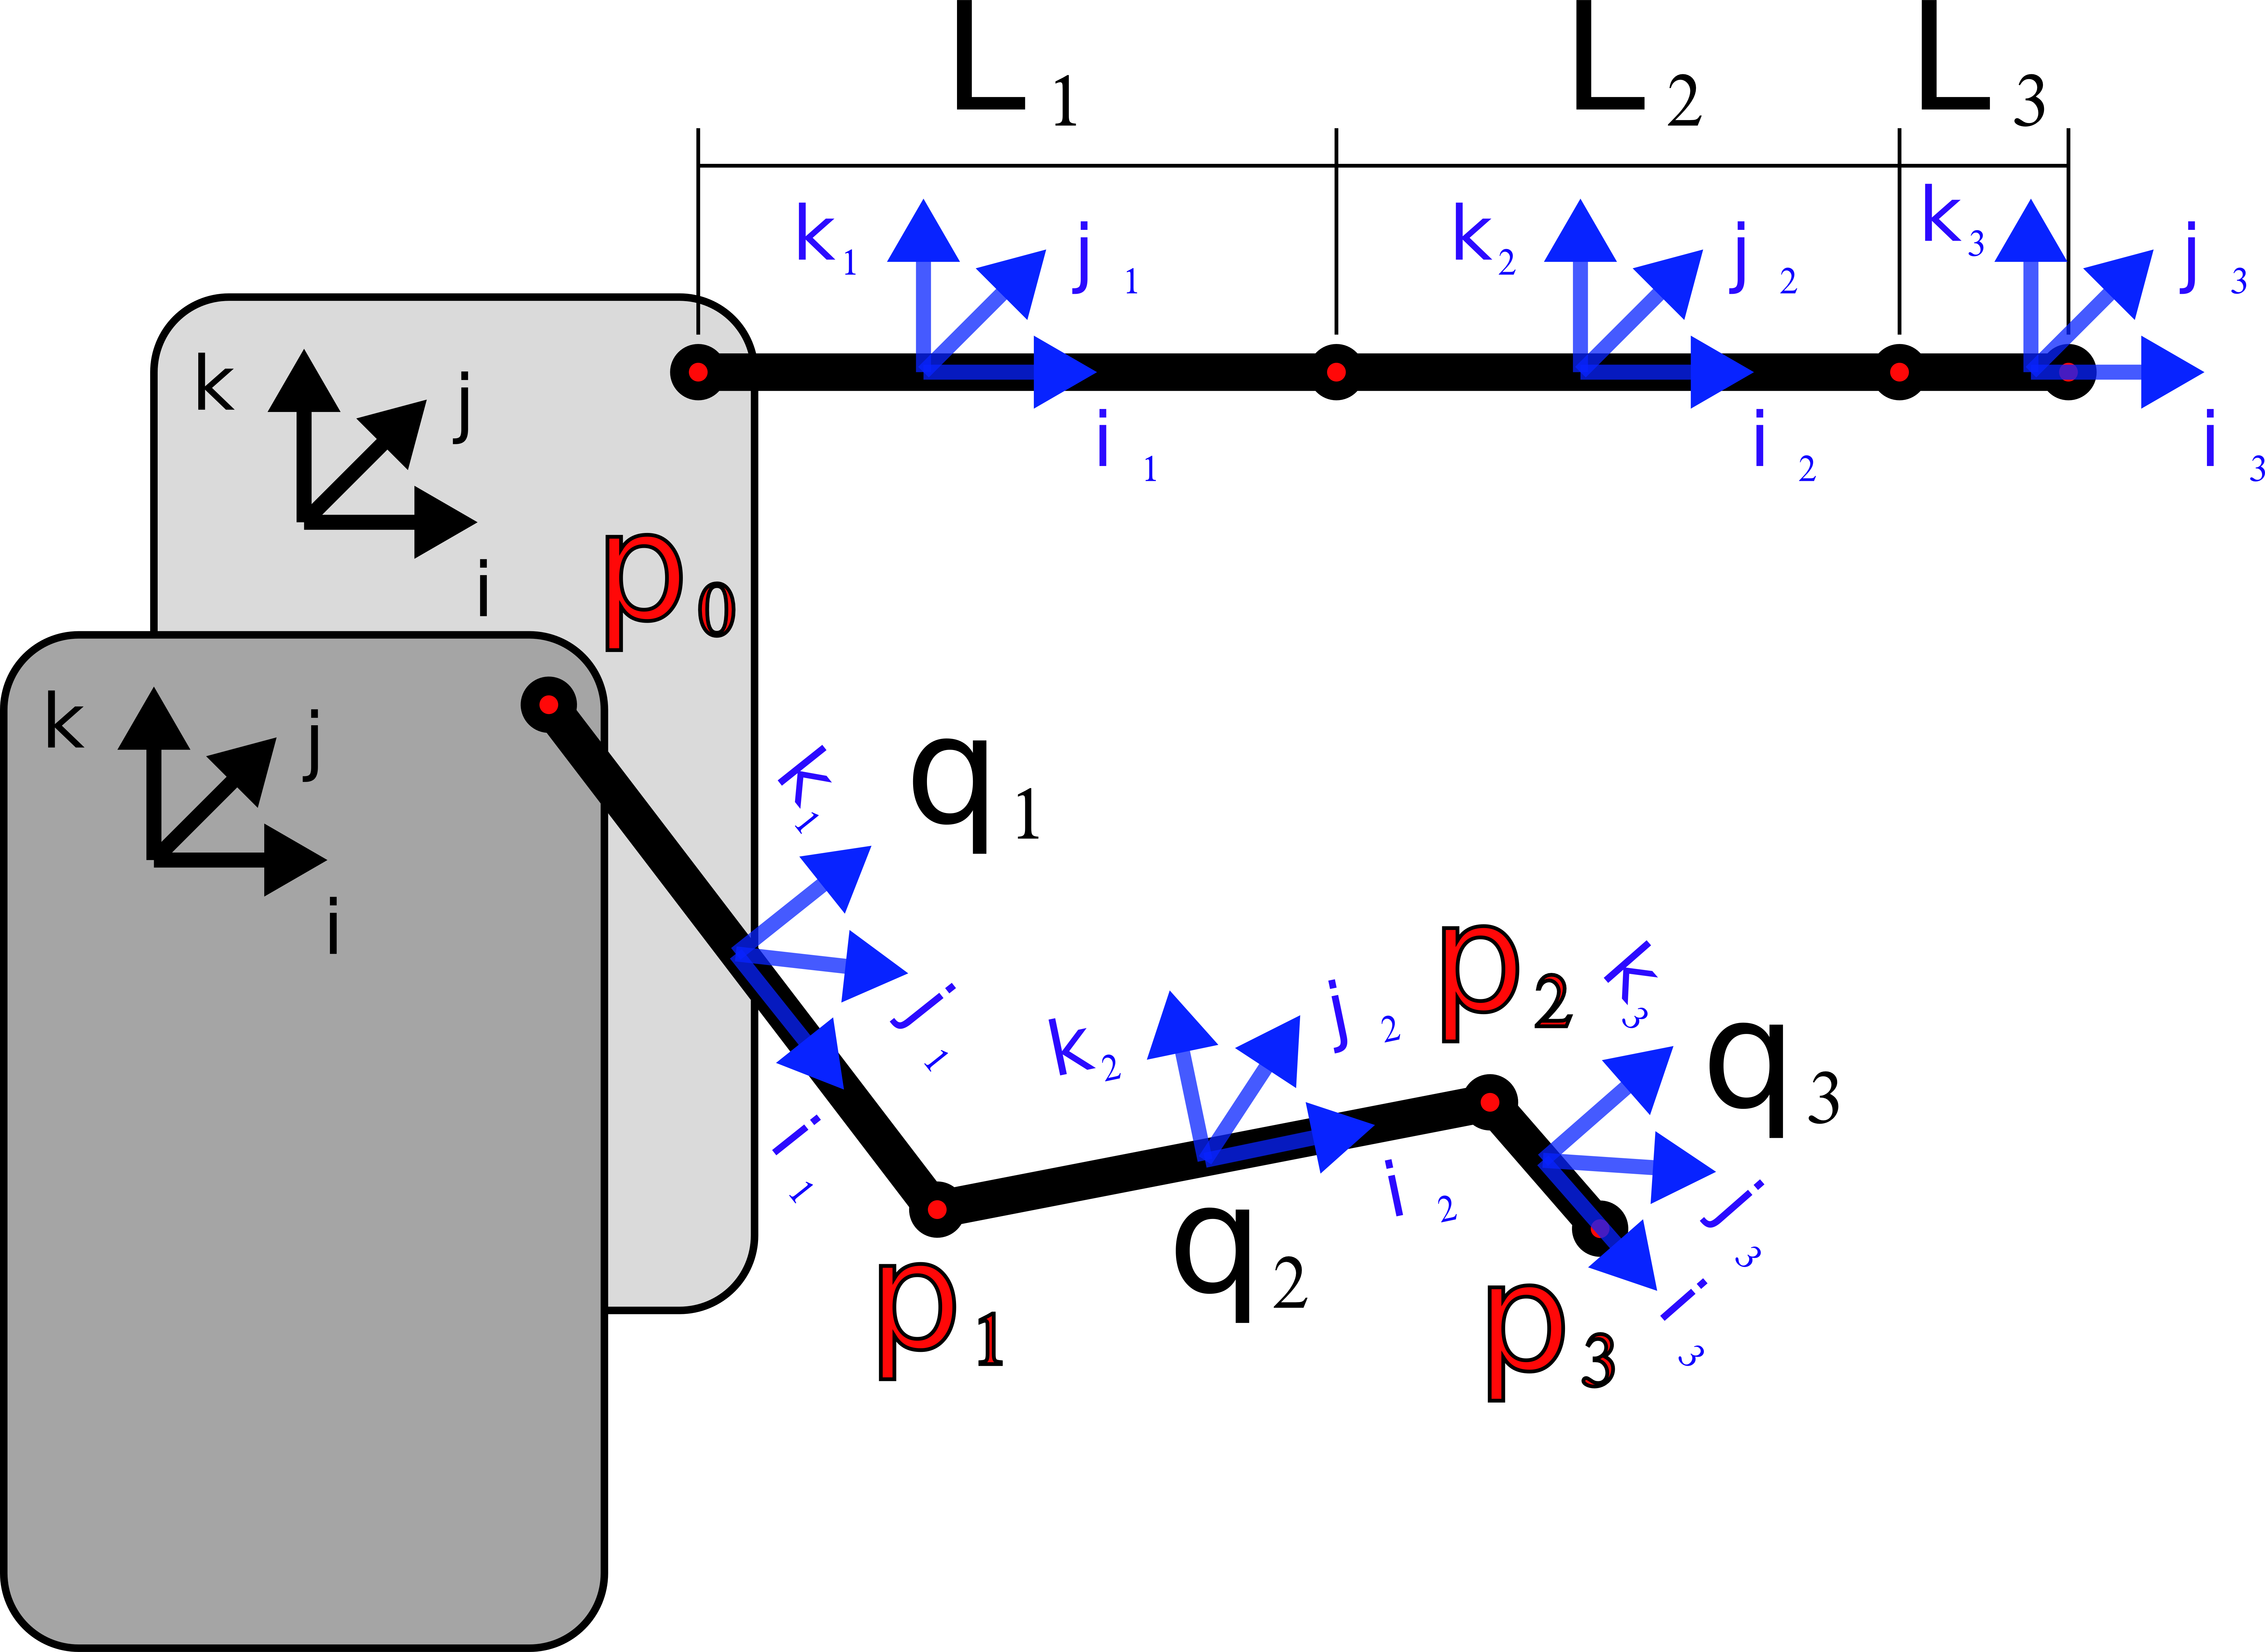
\includegraphics[scale=0.6]{../img/arm_position.png} 
	\caption[Posiciones del brazo inicial y genérica]{Posiciones del brazo inicial y genérica. $L_1$, $L_2$ y $L_3$ son las longitudes de brazo, antebrazo y mano respectivamente, y $q1$, $q2$ y $q_3$ son sus respectivas orientaciones. $p_0$, $p_1$, $p_2$ y $p_3$ son las posiciones de hombro, codo, muñeca y punta de dedo respectivamente.}
	\label{fig: posiciones_brazo}
\end{figure}

Dada una posición genérica del brazo definida por el conjunto de cuaterniones $\{q_i\} = \{q_1, q_2, q_3\}$, las posiciones de cada articulación se pueden calcular de esta forma:

$$ \text{Hombro:} \quad p_0 = 0 $$
$$ \text{Codo:} \quad p_1 = q_1(L_1i)q_1^* $$
$$ \text{Muñeca:} \quad p_2 = p_1 + q_2(L_2i)q_2^* $$
$$ \text{Punta de dedo:} \quad p_3 = p_2 + q_3(L_3i)q_3^* $$

Además se pueden obtener las posiciones local y global de un punto cualquiera $r$ (no necesariamente articulación) perteneciente a un eslabón $K$, del que se conoce su posición local inicial $r_L^i$:

$$ r_L = q_Kr_L^iq_K^* $$
$$ r_G = p_{K-1} + r_L = p_{K-1} + q_Kr_L^iq_K^* $$

donde $p_{K-1}$ es la posición de la articulación $K-1$. Se puede generalizar este resultado a la posición de un punto $r$ cualquiera situado en la articulación $K$ de un brazo articulado, no necesariamente humano, con $N$ eslabones, definido por las longitudes de los eslabones $\{L_i\} = \{L_1, L_2, \ldots , L_N\}$ y orientaciones $\{q_i\} = \{q_1, q_2, \ldots, q_N\}$:

$$ r_G = p_{K-1} + q_Kr_L^iq_K^* = p_{K-2} +  q_{K-1} (L_{K-1}i) q_{K-1}^* + q_K r_L^i q_K^* = \ldots $$

\begin{equation}
r_G = q_Kr_L^iq_K^* + \sum\limits_{m = 1}^{K-1} q_m (L_mi) q_m^*
\end{equation}

donde $r_L^i$ es la posición local inicial de $r$ dentro del eslabón.

\section{Obtención de los ángulos de Euler a partir del cuaternión de orientación}

En ciertas aplicaciones, como por ejemplo cuando se pretende mover las articulaciones de un brazo robótico, resultan más útiles los ángulos de Euler que el cuaternión o la matriz de rotación. Normalmente los brazos robóticos presentan articulaciones de un grado de libertad en las que la característica que define el estado de la articulación es el ángulo. Se puede definir un estado de rotación mediante tres ángulos --ángulos de Euler-- sobre tres los tres ejes principales $x, y, z$. A estas rotaciones se les denomina rotaciones principales. En este apartado se verá como realizar el cálculo de los ángulos de Euler a partir del cuaternión de rotación. \\

Para la obtención de los ángulos de Euler se usará la convención para los ángulos $<\psi: yaw (Z),\, \theta: pitch (Y),\, \phi: roll (X)>$ en un sistema de coordenadas intrínsecas, lo que equivale a $<\phi, \theta, \psi>$ en coordenadas extrínsecas. Se supondrá el sistema de coordenadas local situado sobre la superficie de una esfera de radio unitario, con un sistema de coordenadas global, de tal modo que el eje $x$ del sistema de coordenadas local sea siempre normal a la superficie de la esfera y el eje $z$ se tomará por el momento apuntando al norte de la esfera y paralelo a su superficie. Se tomará como origen de coordenadas ($O$) la posición en que coinciden los sistemas de coordenadas local y global.\\

\begin{figure}[h]
	\centering
		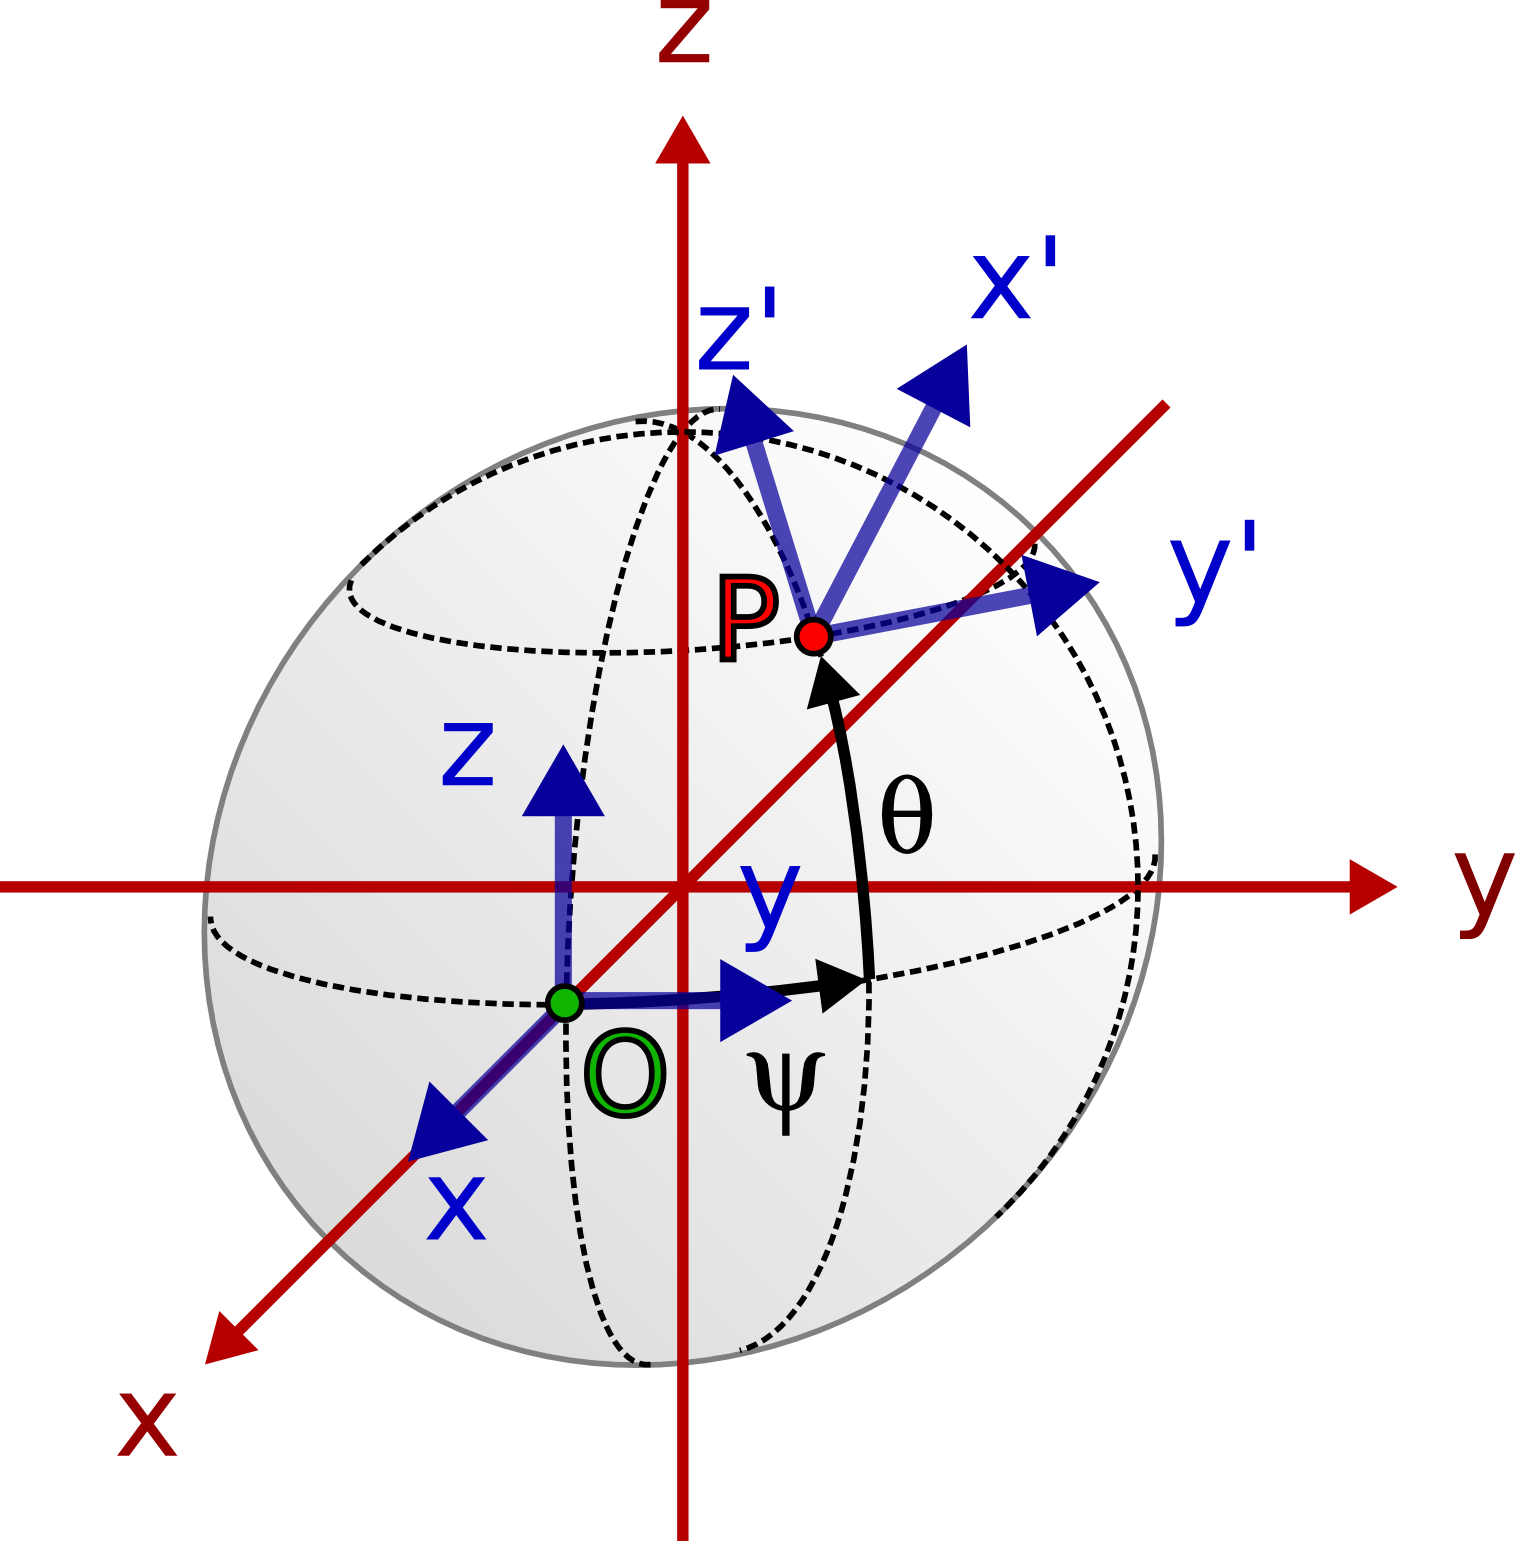
\includegraphics[scale=0.85]{../img/sphere.png} 
	\caption{Sistema de coordenadas local sobre la esfera}
	\label{fig: esfera_coordenadas}
\end{figure}

Se mueve un punto desde el origen de coordenadas $O$ hasta un punto $P$, tal como se muestra en la figura \ref{fig: esfera_coordenadas}. El punto $P$ tiene por coordenadas:

$$ P = \cos \psi \cos \theta i + \sin \psi \cos \theta j + \sin \theta k$$

Como la esfera es de radio unitario, resulta obvio que el punto $P$ tiene las mismas coordenadas que el vector $i'$ perteneciente al sistema de coordenadas local, si éste tuviera por origen el centro de la esfera.

\begin{equation} \label{eq: E13}
i' = \cos \psi \cos \theta i + \sin \psi \cos \theta j + \sin \theta k
\end{equation}

Utilizando las componentes del vector $i'$ resulta sencillo obtener los ángulos $\psi$ y $\theta$:

\begin{equation}
\frac{i'_y}{i'_x} =  \frac{\sin \psi \cos \theta}{\cos \psi \cos \theta} = \tan{\psi} \iff \psi = \arctan \left( \frac{i'_y}{i'_x} \right)
\end{equation}

\begin{equation}
i'_z =  \sin \theta \iff \theta = \arcsin i'_z
\end{equation}

A continuación se realiza la tercera rotación sobre el eje $x'$. Los ejes $y''$ y $z''$ así obtenidos permanecerán tangentes a la superficie de la esfera, mientras el eje $x''$ coincidirá con $x'$. Esta situación final se muestra en la figura \ref{fig: esfera_local}.\\

\begin{figure}[h]
	\centering
		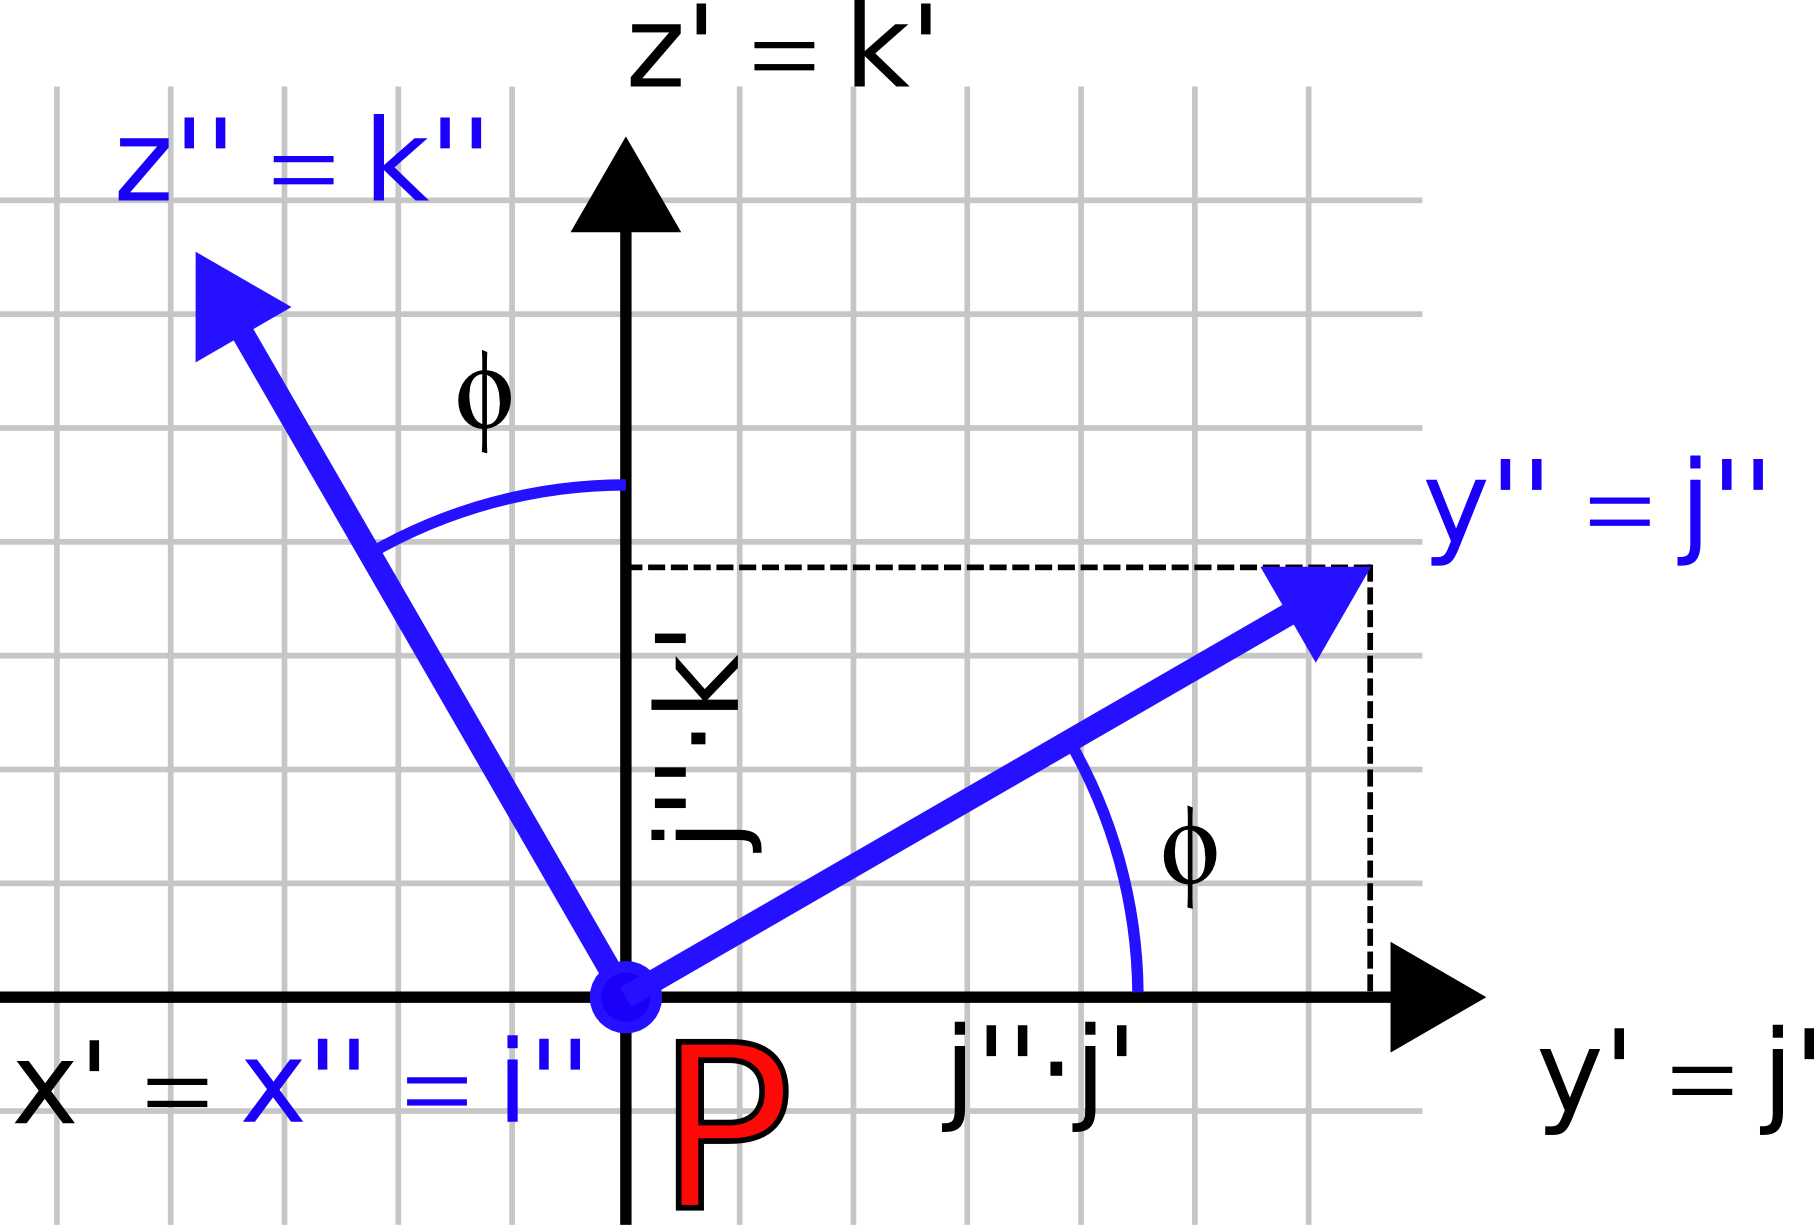
\includegraphics[scale=2]{../img/sphere_local.png} 
	\caption{Tercera rotación en el sistema de coordenadas local sobre el punto P de la esfera}
	\label{fig: esfera_local}
\end{figure}

El estado del sistema de coordenadas tras la tercera rotación es el que va a ser dado por el cuaternión de orientación que nos proporciona el sensor, al que se denominará $q_s$. Sin embargo, para el cálculo del último de los ángulos ($\phi$) se necesitará conocer el hipotético estado anterior a dicha rotación. Sabiendo que el vector $i''$ es igual a $i'$, es posible obtener el sistema de coordenadas en el estado intermedio.\\

El sistema de coordenadas final es el siguiente:

$$ \begin{cases}
i'' = q_siq_s^* = i''_x i + i''_y j + i''_z k \\
\\
j'' = q_sjq_s^* = j''_x i + j''_y j + j''_z k \\ 
\\
k'' = q_skq_s^* = k''_x i + k''_y j + k''_z k 
\end{cases}$$

Para el cálculo del conjunto $\{i', j', k'\}$ se parte de que $i' = i''$. Además se sabe que el vector $j'$ será perpendicular a $k$ y a la proyección de $i''$ sobre el plano $xy$ de la esfera. Esta proyección será la resultante de eliminar la componente en $k$ de $i''$:

$$ i''_{xy} = i''_x i + i''_y j $$

De la ecuación \eqref{eq: E13} se puede deducir que el módulo de la proyección de este vector será:

$$ \|i''_{xy}\| = \sqrt{\left(\cos \psi \cos \theta\right)^2 + \left(\sin \psi \cos \theta \right)^2} = \cos\theta$$

Para el cálculo de $j'$ será necesario utilizar el vector $i''_{xy}$ normalizado ya que si no se obtendría un vector cuyo módulo no sería unitario: 

$$ \left( i''_{xy} \right)_u = \frac{i''_{xy}}{\cos\theta} = \frac{1}{\cos\theta}\left( i''_x i + i''_y j \right) $$

Ahora se puede calcular $j'$:

$$ j' = k \times \left( i''_{xy} \right)_u = \frac{1}{\cos\theta} k \times\left( i''_x i + i''_y j \right) $$

\begin{equation}
j' = \frac{1}{\cos\theta} \left( - i''_y i + i''_x j \right)
\end{equation}
  
Finalmente, una vez conocidos $i'$ y $j'$, es posible obtener $k'$:

$$ k' = i' \times j' $$

En resumen:

\begin{equation}
\begin{cases}
i' = i''_x i + i''_y j + i''_z k \\
\\
j' = \displaystyle\frac{1}{\cos\theta} \left( - i''_y i + i''_x j \right) \\
\\
k' = i' \times j'
\end{cases}
\end{equation}

Finalmente, conociendo el vector $j'$ se puede obtener el último de los ángulos buscados:

\begin{equation}
\tan\phi = \frac{\sin \phi}{\cos \phi} = \frac{j'' \cdot k'}{j'' \cdot j'} \quad \iff \quad \phi = \arctan \frac{j'' \cdot k'}{j'' \cdot j'}
\end{equation}

El algoritmo de cálculo de los ángulos de Euler puede resumirse en los siguientes pasos, conocido el cuaternión de orientación del sensor $q_s$ \footnote{A la hora de implementar el algorimo, se utilizará la función atan2 en lugar de $\arctan$}:

\begin{table}[h]
	\center
	\begin{tabular}{|l|l|c|}
	\hline
	\multicolumn{3}{|c|}{\textbf{Algoritmo de cálculo de los ángulos de Euler}}\\
	\multicolumn{3}{|c|}{\textbf{a partir del cuaternión de orientación}}\\
	\hline
	1º & Cálculo de $i''$ y $j''$ & $ i' = i'' = q_siq_s^* \quad j'' = q_sjq_s^*$  \\
	2º & Obtención de los ángulos $\psi$ y $\theta$ & $ \psi = \arctan \left( \displaystyle\frac{i'_y}{i'_x} \right) \quad \theta = \arcsin i'_z $ \\
	3º & Cálculo del vector $j'$ y $k'$ & $ j' = \displaystyle\frac{1}{\cos\theta} \left( - i''_y i + i''_x j \right) \quad k' = i' \times j' $ \\
	4º & Obtención del tercer ángulo, $\phi$ & $ \phi = \arctan \displaystyle\frac{j'' \cdot k'}{j'' \cdot j'} $ \\
	\hline
	\end{tabular}

	\caption{Algoritmo de cálculo de los ángulos de Euler a partir del cuaternión de orientación.}
	\label{tab:algoritmo_angulos_euler}

\end{table}

\subsection{Ampliación del intervalo de los ángulos obtenidos}

El algoritmo presentado en el cuadro \ref{tab:algoritmo_angulos_euler} da una solución para el ángulo $\theta$ dentro del intervalo $\left(-\frac{\pi}{2}, \frac{\pi}{2} \right)$. Puede pasar que la articulación del brazo robótico cuyo eje se refiera al ángulo $\theta$ se mueva en un intervalo más amplio. O que se quieran mover únicamente dos articulaciones mediante un sensor prescindiendo de la tercera rotación, y se necesite que $\phi \approx 0$ ya que de otro modo los otros dos ángulos no se corresponden muy bien con la realidad. por ello resultará de interés poder obtener soluciones de $\theta$ que no se restrinjan al intervalo $\left(-\frac{\pi}{2}, \frac{\pi}{2} \right)$. En los apartados siguientes se dará un par de posibles soluciones a este problema.

\subsubsection{Generación de una segunda solución a partir de la primera}

Si se amplía el intervalo de $\theta$ a $(-\pi, \pi)$, se obtiene que cada posición en la esfera puede representarse de dos formas distintas mediante los ángulos $\psi$ y $\theta$. \\

\begin{figure}[h]
	\centering
		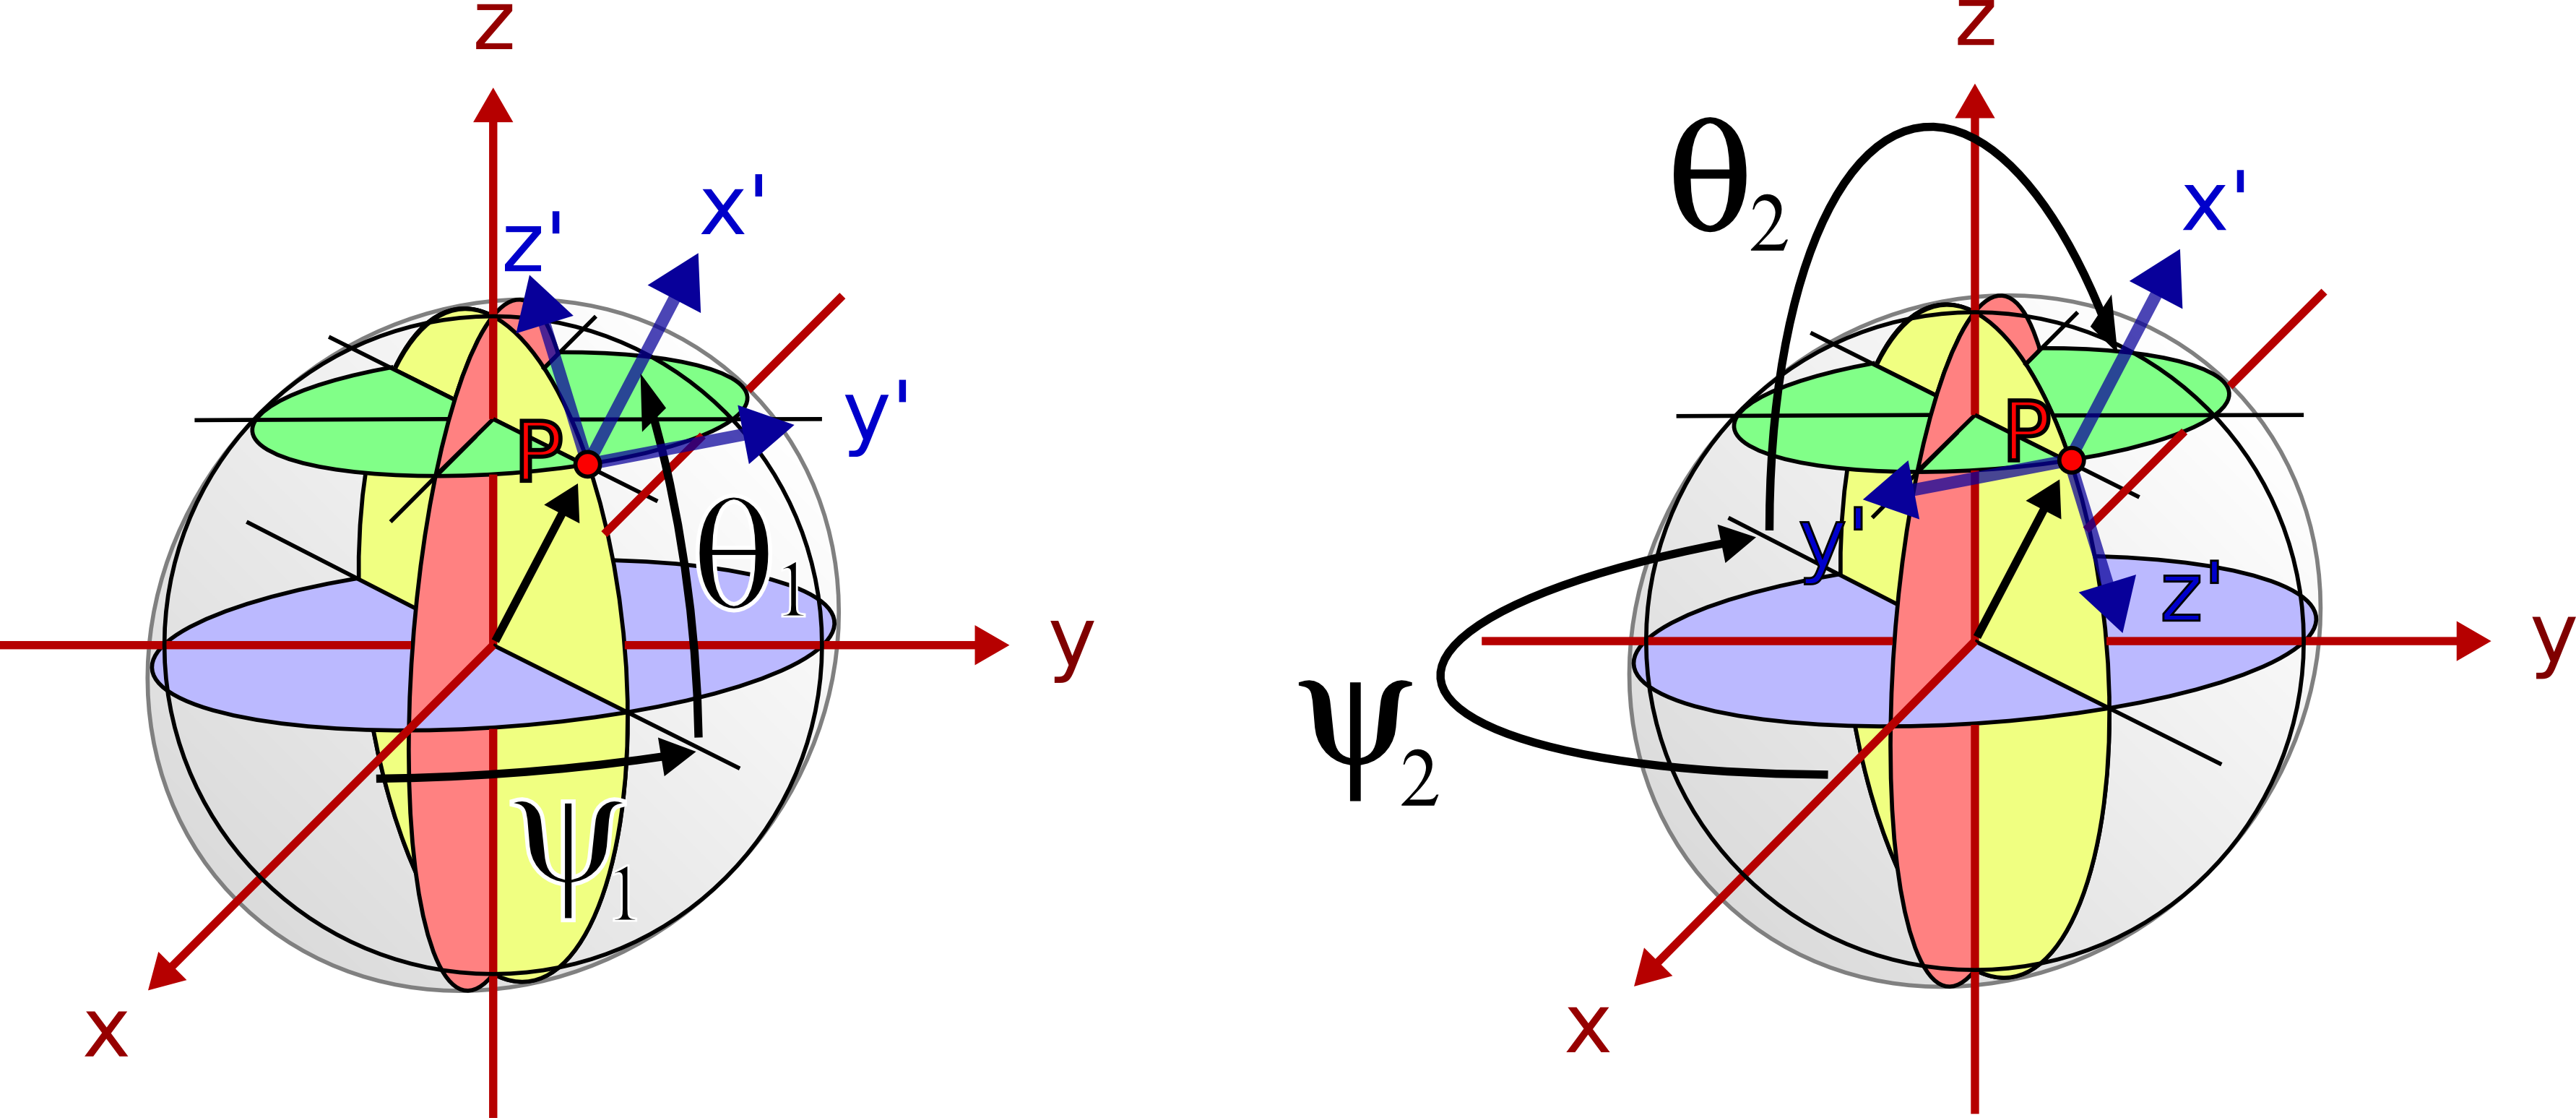
\includegraphics[scale=0.85]{../img/ea_solutions.png} 
	\caption{Dos soluciones para $\theta$ (\textit{pitch}) y $\psi$ (\textit{yaw})} 
	\label{fig: dos_soluciones_esfera}
\end{figure}

En la figura \ref{fig: dos_soluciones_esfera}) se muestran los ángulos de las dos posibles soluciones. Sea una solución $s_1 = \{ \psi_1, \theta_1, \phi_1 \}$ obtenida mediante el algoritmo descrito en el cuadro \ref{tab:algoritmo_angulos_euler}; Se deduce que la segunda solución es:

$$ s_2 = \begin{cases}

\psi_2 = \begin{cases}
	\psi_1 + \pi : \quad \psi_1 < 0 \\
	\psi_1 - \pi : \quad \psi_1 \geq 0 
\end{cases}\\
\\
\theta_2 = \begin{cases}
	-\pi - \theta_1 : \quad \theta_1 < 0 \\
	\pi - \theta_1 : \quad \theta_1 \geq 0 
\end{cases}\\
\\
\phi_2 = \begin{cases}
	\phi_1 + \pi : \quad \phi_1 < 0 \\
	\phi_1 - \pi : \quad \phi_1 \geq 0 
\end{cases}
\end{cases}
$$

Para decidir que solución será la buena se deberá establecer un criterio de selección. Por ejemplo, en el caso de querer mover dos articulaciones, se sabe que $\phi$ tiene que ser aproximadamente $0$. En el momento en que la primera solución nos de un valor de $\phi$ muy diferente de $0$, se escogerá la segunda solución.\\

En la práctica, este método funciona bastante bien siempre y cuando $\theta \not\approx \frac{\pi}{2}$. En esta zona de la esfera se tiene que $\cos\theta \approx 0$, y a la hora de calcular $ j'$ (\ref{tab:algoritmo_angulos_euler}), el término $\frac{1}{\cos\theta}$ amplifica enormemente el ruido propio del sensor, lo que genera saltos de magnitud apreciable en los valores de los ángulos obtenidos, aún cuando el sensor permanece estático.

\subsubsection{Permutación de los ejes locales}

Sea una articulación cuyo eje de rotación coincida con el eje $y$ de los dos sensores dispuestos para medir su estado. Es esta situación se deduce de antemano que el vector base $i$ local siempre se localizará en torno a un circulo máximo de la esfera, por lo que habrá zonas en las que nunca se situará. \\ 

\colorbox{red}{FALTA}

\chapter{IMPLEMENTACIÓN DEL SOFTWARE}

En este capítulo se describirá detalladamente el funcionamiento de los programas realizados para el presente proyecto. Todo el software se ha incluido dentro de un \textit{stack} de ROS --llamado youbot-xsens-controller--, de forma que su instalación \footnote{Se describirá el proceso de instalación en el anexo \textit{INSTALACIÓN Y PUESTA EN MARCHA DEL SOFTWARE}} en otros ordenadores con ROS sea sencilla y rápida.\\

El stack \textit{youbot-xsens-controller} está compuesto por los siguientes paquetes, que pueden instalados de forma independiente si así se deseara:

\begin{itemize}

\item \textbf{xsens\_driver}: driver para la comunicación sensor/máster - PC

\item \textbf{dfv}: librería para el manejo de cuaterniones, vectores y matrices.

\item \textbf{youbot\_controller}: programa que realiza el control del robot \textit{Youbot} utilizando los datos de los sensores \textit{xsens}.

\end{itemize}

Para la creación de los distintos programas se han utilizado las herramientas que proporciona ROS para la compilación de programas y gestión de paquetes. En la figura \ref{fig: communications} se presenta un esquema simplificado de las comunicaciones entre los distintos programas que forman el sistema.

\begin{figure}[h]
	\centering
		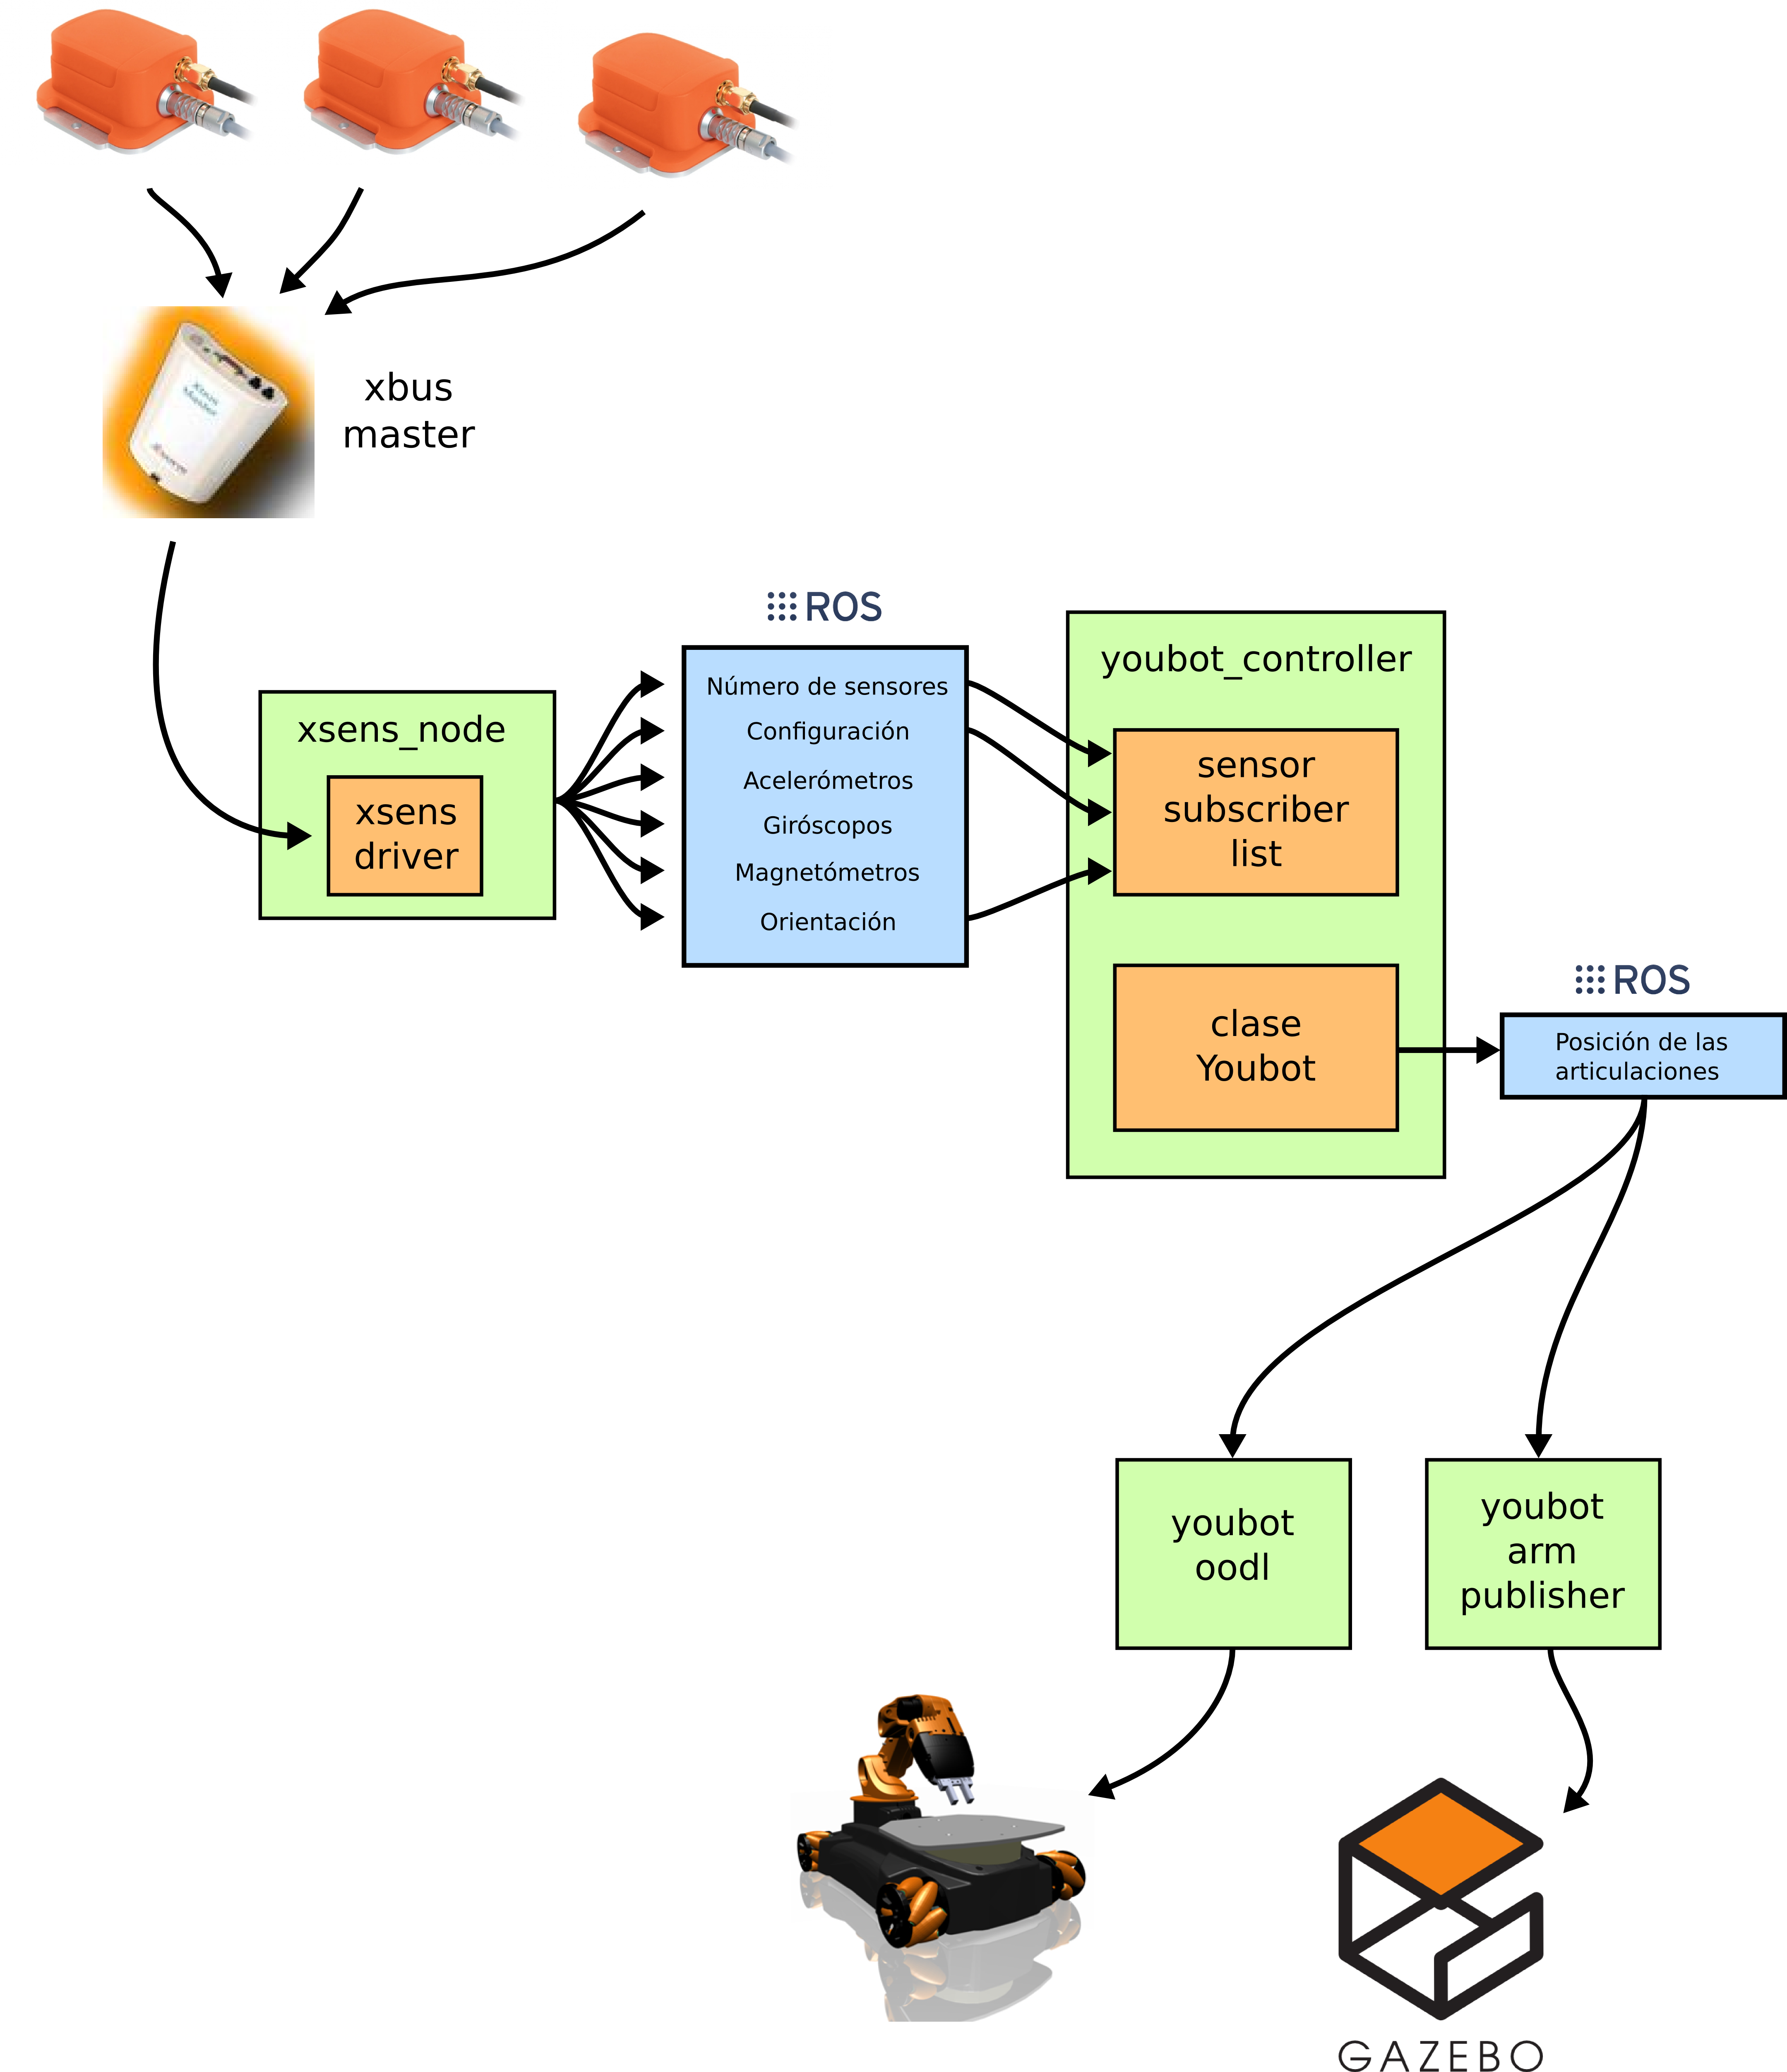
\includegraphics[scale=0.30]{../img/communications.png} 
	\caption[Esquema simplificado de comunicaciones]{Esquema simplificado de las comunicaciones entre programas. En azul se representan los topics y parámetros de ROS, en verde los nodos y en naranja las clases principales. } 
	\label{fig: communications}
\end{figure}


\section{Driver para la comunicación xbus Master/xsens - PC}

Uno de los problemas más importantes a resolver en este proyecto es conseguir una comunicación fluida de los datos de los sensores hacia el PC. La comunicación entre un dispositivo y el ordenador se realiza mediante un programa llamado \textit{driver}, que actúa de interfaz entre el dispositivo físico y el sistema operativo del PC, utilizando algún tipo de canal de datos (USB, bluetooth, etc.). En el caso del driver para los sensores xsens, la comunicación se realizará a través del puerto USB.\\

En la documentación del \textit{Kit de Desarrollo de Software} de \textit{xsens} vienen proporcionadas algunas clases y estructuras en lenguaje C++ para la comunicación de bajo nivel con el sensor/máster. Para la realización del driver se han aprovechado estas clases y se han encapsulado dentro de una clase \textit{wrapper}, llamada \textit{xsens::Driver}, que proporciona una interfaz sencilla hacia las clases de bajo nivel. El programa principal del \textit{driver} realiza la configuración de los sensores, y lee los datos a través del \textit{wrapper}, publicándolos en \textit{topics} de ROS.\\

Los archivos de la documentación que se han incluído en el driver son los siguientes (incluyen los archivos de extensión .cpp y .h):

\begin{itemize}

\item cmt1: implementa las comunicaciones de bajo nivel con el puerto serie.
\item cmt2: interfaz para mensajes y ficheros de registro.
\item cmt3: capa de más alto nivel para las comunicaciones con el sensor. Proporciona una interfaz independiente del sistema operativo.
\item cmtdef: definiciones de constantes y tipos de datos.
\item cmtmessage: gestión de mensajes.
\item cmtpacket: gestión de los paquetes de información en los que se basa la comunicación entre el sensor y el PC.
\item cmtscan: funciones para el escaneo de los puertos del PC.
\item pstdint: una versión portable de la librería stdint, que incluye definiciones precisas de tipos de datos enteros. 
\item xsens\_exception: definición de la clase Exception usada por el driver.
\item xsens\_fifoqueue: contiene la implementación de una cola FIFO.
\item xsens\_file: definición de algunos tipos de datos.
\item xsens\_janitors: implementación de distintos tipos de \textit{janitors}, que realizan funciones de limpieza de objetos al perder su \textit{scope}.
\item xsens\_list: implementación de una clase lista utilizada en el driver.
\item xsens\_std: definición de los valores de retorno de las funciones del driver.
\item xsens\_time: implementación de funciones y constantes para la gestión del tiempo.

\end{itemize}

En la siguiente lista se muestran los archivos creados en este paquete y la función que realizan dentro del driver:

\begin{itemize}
\item xsens\_driver: implementación de la clase \textit{xsens::Driver}, la cual básicamente realiza una encapsulación de todas las clases que se incluyen en los archivos mencionados en la lista anterior y actúa de interfaz con el nodo principal \textit{xsens\_node}.
\item xsens\_sensor: la clase xsens::Sensor es en esencia una estructura de datos donde se almacena la configuración de cada uno de los sensores conectados y los datos leídos en cada ciclo de lectura.
\item xsens\_node: programa principal del driver. Se encarga de publicar en ROS los datos leídos a través de la clase \textit{xsens::Driver}.
\item xsens\_sensor\_subscriber: no pertenece al driver propiamente dicho, sino que este archivo es parte de la implementación de la librería \textit{xsens\_driver} que puede utilizarse como interfaz de lectura en otros programas de los datos publicados por el driver.
\end{itemize}

A continuación se realiza una descripción en detalle de la implementación y funcionamiento del driver.

\subsection{Funcionamiento de la clase xsens::Driver}

La clase \textit{xsens::Driver} actúa de interfaz hacia las clases de más bajo nivel encargadas de la comunicación del puerto serie. El objetivo perseguido con su creación es encapsular y automatizar la configuración de los sensores y la lectura de datos, de forma que no sea necesario realizar todo este proceso manualmente. Resumiendo brevemente, las funciones que realiza esta clase son:

\begin{enumerate}

\item Realizar un escaneo de los puertos USB del PC con el objetivo de detectar tipo y número de sensores conectados.

\item Configurar los sensores en el modo deseado (datos que devolverá, forma de representar las orientaciones, etc.).

\item Establecer los sensores en modo de medición.

\item Actualizar los datos miembro cada vez que llega una nueva medición de los sensores.

\end{enumerate}

Esta clase contiene una serie de métodos miembro que permiten interactuar con ella. En la siguiente lista se muestran los de mayor utilidad:

\begin{itemize}

	\item Métodos para establecer la configuración del sensor:

	\begin{itemize}
	
		\item \textbf{void SetOutputMode(CmtOutputMode output\_mode)}\\
		Permite establecer el modo de salida del sensor, el cual define el tipo de datos que devolverá. Acepta un parámetro de tipo \textit{CmtOutputMode}, que puede ser combinación de varios de los siguientes valores:
		
		\begin{itemize}
		
			\item CMT\_OUTPUTMODE\_RAW: datos crudos de los acelerómetros, giróscopos y magnetómetros sin calibrar.
			\item CMT\_OUTPUTMODE\_TEMP: temperatura registrada por el sensor.
			\item CMT\_OUTPUTMODE\_CALIB: datos calibrados de los acelerómetros, giróscopos y magnetómetros.
			\item CMT\_OUTPUTMODE\_ORIENT: orientación del sensor.
		
		\end{itemize}
		
		Por ejemplo, para configurar el sensor de modo que devuelva los datos calibrados, la orientación y la temperatura se llamará a la función de la siguiente forma:
		
		\begin{lstlisting}[language=C++]
driver.SetOutputMode(CMT_OUTPUTMODE_CALIB | CMT_OUTPUTMODE_ORIENT | CMT_OUTPUTMODE_TEMP);
		\end{lstlisting}
		
		\item \textbf{void SetOutputSettings(CmtOutputSettings output\_settings)}\\
		Permite establecer la forma de representación de la orientación del sensor. Acepta un parámetro de tipo \textit{CmtOutputSettings}, que puede ser uno de los siguientes valores:
		
		\begin{itemize}
		
			\item CMT\_OUTPUTSETTINGS\_ORIENTMODE\_EULER: Orientación del sensor en forma de ángulos de Euler
			\item CMT\_OUTPUTSETTINGS\_ORIENTMODE\_MATRIX: Matriz de rotación.
			\item CMT\_OUTPUTSETTINGS\_ORIENTMODE\_QUATERNION: Cuaternión de orientación.
		
		\end{itemize}
		
		Para configurar el sensor de modo que devuelva su orientación forma de cuaternión, se pasará a la función el siguiente parámetro:
		
		\begin{lstlisting}[language=C++]
driver.SetOutputSettings(CMT_OUTPUTSETTINGS_ORIENTMODE_QUATERNION);
		\end{lstlisting}
		
		\item \textbf{void SetAlignmentMatrix(unsigned int sensor\_index, CmtMatrix alignment\_matrix)}\\
		Establece una matriz de rotación inicial al sensor cuyo identificador se le pase al parámetro \textit{sensor\_index} sensor\_index.
		
		Para establecer una matriz de rotación inicial identidad al sensor de id 0:
		
		\begin{lstlisting}[language=C++]
driver.SetAlignmentMatrix(0, xsens::DfvToCmtMatrix(dfv::Matrix::Identity(3)));
		\end{lstlisting}
		
		\item \textbf{bool Initialize()}\\
		Se llamará a esta función después de haber establecido los parámetros del sensor mediante las funciones descritas anteriormente. Esta función pone al sensor en modo configuración, lo prepara para que devuelva los datos deseados y lo pone en modo de medida.		
	
	\end{itemize}
	
	\item Métodos para leer datos del sensor:

	\begin{itemize}
		
		\item \textbf{unsigned int GetMtCount()}\\
		Devuelve el número de dispositivos xsens conectados al PC, excluyendo el máster xbus.		
		
		\item \textbf{CmtOutputMode GetOutputMode() const}\\
		Devuelve el modo de salida de los sensores. Los valores de retorno son los mismos que los que puede aceptar el parámetro de la función \textit{SetOutputMode()} descrita anteriormente.	
		
		\item \textbf{CmtOutputSettings GetOutputSettings() const}	\\
		Devuelve la forma de representación de la orientación de los sensores. Los valores de retorno son los mismos que los que puede aceptar el parámetro de la función \textit{SetOutputSettings()} descrita anteriormente.		
				
		\item \textbf{bool SpinOnce()}\\
		Esta función realiza un ciclo en la toma de datos del sensor. Se queda esperando a que llegue un mensaje procedente del sensor, y a continuación actualiza todas las estructuras de datos con los nuevos valores obtenidos. Se ha de llamar a esta función antes de ejecutar alguna de las funciones descritas a continuación. Devuelve \textit{true} si todos los datos fueron leídos de forma correcta, y \textit{false} en caso contrario.
		
		\item \textbf{CmtQuat\& GetOriQuat(int mt\_index = 0)}\\
		Devuelve el cuaternión de orientación del sensor con número de identificación especificado. Si se deja el parámetro en blanco, devuelve el cuaternión de orientación del sensor de id 0.
		
		\item \textbf{CmtMatrix\& GetOriMatrix(int mt\_index = 0)}\\
		Devuelve la matriz de orientación del sensor con número de identificación especificado. Si se deja el parámetro en blanco, devuelve la matriz de orientación del sensor de id 0.
		
		\item \textbf{CmtEuler\& GetOriEuler(int mt\_index = 0)}\\
		Devuelve los ángulos de Euler del sensor con número de identificación especificado. Si se deja el parámetro en blanco, devuelve los ángulos de Euler del sensor de id 0.
		
		\item \textbf{CmtRawData\& GetRawData(int mt\_index = 0)}\\
		Devuelve los datos crudos de los acelerómetros, giróscopos y magnetómetros, además de la temperatura del sensor con número de identificación especificado. Si se deja el parámetro en blanco, devuelve los datos crudos del sensor de id 0. Los datos crudos contienen los datos de salida de los conversores analógico-digitales de los sensores, y tienen la forma de enteros de 16 bits. Los datos de los acelerómetros, giróscopos y magnetómetros están compuestos cada uno de un vector de 3 enteros de 16 bits (ejes XYZ), y la temperatura es otro entero de 16 bits.	
		
		\item \textbf{CmtCalData\& GetCalData(int mt\_index = 0)}\\
		Devuelve los datos calibrados de los acelerómetros, giróscopos y magnetómetros del sensor con número de identificación especificado. Si se deja el parámetro en blanco, devuelve los datos calibrados del sensor de id 0.	

\begin{table}[h]
\center
\begin{tabular}{|l|l|l|}
\hline
\multicolumn{3}{|c|}{\textbf{Datos calibrados de los sensores}}\\
\hline
\textbf{Dato} & Tipo & \textbf{Unidades} \\ 
\hline
acelerómetros & array de 3 floats & $\displaystyle\frac{m}{s^2}$ \\
giróscopos & array de 3 floats & $\displaystyle\frac{rad}{s}$ \\
magnetómetros & array de 3 floats & $mGauss$ \\
temperatura & float & $^\circ C$ \\
\hline
\end{tabular}	
\caption[Unidades de los datos calibrados devueltos por los sensores]{Unidades de los datos calibrados devueltos por los sensores.}
\label{tab:sensor_units}	
\end{table}		
			
	\end{itemize}

\end{itemize}

A continuación se presenta un ejemplo mínimo de cómo utilizar la clase xsens::Driver para tomar datos de un sensor:

\lstset{inputencoding=utf8/latin1}
\lstinputlisting[language=C++]{../src/xsens_driver_example.cpp}


\subsection{Programa principal: xsens\_node}

El nodo \textit{xsens\_node} es el encargado de publicar en topics de ROS los datos leídos de los sensores. Para la lectura de los datos del sensor hace uso de la clase xsens::Driver descrita en el apartado anterior. Podría considerarse que este programa actúa de interfaz entre dicha clase y ROS. Este programa realiza las siguientes tareas:

\begin{enumerate}

	\item Detección del número de sensores conectados al PC.
	
	\item Configuración de los sensores:
	
	\begin{itemize}
	
		\item Modo de salida: datos calibrados y orientación.
		\item Forma de representación de la orientación: cuaternión.
		\item Matriz de rotación inicial identidad.	
	
	\end{itemize}
	
	\item Inicialización y creación de los topics y parámetros de ROS. En concreto se crean los topics y parámetros descritos en los cuadros \ref{tab:topics_xsens_node} y \ref{tab:params_xsens_node} respectivamente.
	
	\item Lectura de los datos del sensor y publicación en los topics de ROS correspondientes.
		
	
\end{enumerate}

\begin{table}[h]
\footnotesize
\center
\begin{tabular}{|l|l|l|}
\hline
\multicolumn{3}{|c|}{\textbf{Topics}}\\
\hline
\textbf{Nombre} & \textbf{Tipo} & \textbf{Descripción} \\ 
\hline
/xsens\_node/sensorX/acc & geometry\_msgs::Vector3Stamped & Acelerometros calibrados \\
/xsens\_node/sensorX/gyr & geometry\_msgs::Vector3Stamped & Giróscopos calibrados \\
/xsens\_node/sensorX/mag & geometry\_msgs::Vector3Stamped & Magnetómetros calibrados \\
/xsens\_node/sensorX/raw\_acc & geometry\_msgs::Vector3Stamped & Acelerometros crudos \\
/xsens\_node/sensorX/raw\_gyr & geometry\_msgs::Vector3Stamped & Giróscopos crudos \\
/xsens\_node/sensorX/raw\_mag & geometry\_msgs::Vector3Stamped & Magnetómetros crudos \\
/xsens\_node/sensorX/ori\_quat & geometry\_msgs::QuaternionStamped & Cuaternión de orientación \\
/xsens\_node/sensorX/ori\_matrix & std\_msgs::Float64MultiArray & Matriz de orientación \\
/xsens\_node/sensorX/ori\_euler & std\_msgs::Float64MultiArray & Ángulos de Euler \\
\hline
\end{tabular}	
\caption[Topics publicados por el programa xsens\_node]{Topics publicados por el programa xsens\_node. La X en sensorX representa el número de identificación del sensor. Se crea un topic de cada tipo por cada sensor conectado al máster. Los topics creados también dependen de la configuración de los sensores. Por ejemplo, si los sensores son configurados para que den sólo los datos calibrados, no se crearán los topics de orientación.}
\label{tab:topics_xsens_node}	
\end{table}

\begin{table}[h]
\center
\begin{tabular}{|l|l|l|}
\hline
\multicolumn{3}{|c|}{\textbf{Parámetros}}\\
\hline
\textbf{Nombre} & \textbf{Tipo} & \textbf{Descripción} \\ 
\hline
/xsens\_node/sensor\_count & entero & Número de sensores \\
/xsens\_node/output\_mode & entero & Modo de salida \\
/xsens\_node/output\_settings & entero & Forma de representación de la orientación \\
\hline
\end{tabular}	
\caption[Parámetros publicados por el programa xsens\_node]{Prámetros publicados por el programa xsens\_node.}
\label{tab:params_xsens_node}	
\end{table}

\subsection{Cómo tomar datos del sensor desde otro programa}

Junto con el paquete \textit{xsens\_driver} se incluye además una librería con las clases \textit{xsens::SensorSubscriber} y \textit{xsens::SensorSubscriberList}. Estas clases proporcionan una forma muy sencilla de acceder a los topics publicados por el programa \textit{xsens\_node}. Al declarar un objeto del tipo xsens::SensorSubscriberList, automáticamente dicho objeto se autoconfigura leyendo los parámetros de ROS con la información de configuración de los sensores (cuadro \ref{tab:params_xsens_node}) e inmediatamente se pone a leer los datos de los topics correspondientes (cuadro \ref{tab:topics_xsens_node} a excepción de los datos en crudo), sin tener que hacer nada más que pasarle como parámetro el \textit{handle} del nodo en que sea declarado.\\

Un objeto de clase \textit{xsens::SensorSubscriberList} proporciona los siguientes métodos para lectura de datos del sensor:

\begin{itemize}

\item \textbf{unsigned int GetMtCount() const}\\
Devuelve el número de sensores xsens detectados.

\item \textbf{const dfv::Vector3 GetAcc(unsigned int mt\_index) const}\\
Devuelve un vector con los datos de los acelerómetros del sensor de número de identificación que se le pase como parámetro.

\item \textbf{const dfv::Vector3 GetGyr(unsigned int mt\_index) const}\\
Devuelve un vector con los datos de los giróscopos del sensor de número de identificación que se le pase como parámetro.

\item \textbf{const dfv::Vector3 GetMag(unsigned int mt\_index) const}\\
Devuelve un vector con los datos de los magnetómetros del sensor de número de identificación que se le pase como parámetro.

\end{itemize}

Para incluir la librería \textit{xsens\_driver} en otro proyecto se tendrá que incluir la siguiente línea al final del archivo \textit{CMakeLists.txt} del proyecto de ROS:

\begin{lstlisting}
target_link_libraries(nombre_del_ejecutable dfv xsens_driver)
\end{lstlisting}

En el siguiente cuadro se presenta un ejemplo de como usar la clase xsens::SensorSubscriberList para tomar datos de una red de sensores xsens:

\lstset{inputencoding=utf8/latin1}
\lstinputlisting[language=C++]{../src/xsens_sensor_subscriber_example.cpp}

\section{Librería para manejo de cuaterniones, vectores y matrices}

Dentro del paquete \textit{dfv} se ha creado una librería con la implementación de las clases \textit{dfv::Quaternion}, \textit{dfv::Vector3} y \textit{dfv::Matrix}.

\subsection{La clase dfv::Quaternion}

La clase \textit{dfv::Quaternion} es la implementación del concepto de cuaternión y las operaciones que se pueden realizar con él. A continuación se muestra una breve documentación de las operaciones más importantes que se pueden realizar con esta clase.

\begin{itemize}

\item \textbf{Constructores}:

\begin{itemize}
\item \textbf{Quaternion()}: Constructor sin argumentos. Crea un cuaternión cuyas cuatro componentes son nulas.

\item \textbf{Quaternion(double w\_, double x\_, double y\_, double z\_)}: Constructor del cuaternión genérico (ecuación \eqref{eq: gen_quaternion}). Crea un cuaternión cuyas componentes son los valores que se le pasan a modo de argumento.

\item \textbf{explicit Quaternion(const Vector3\& v)}: Constructor del cuaternión asociado al vector $v$ que se le pasa como parámetro (ecuación \eqref{eq: E15}). 
\end{itemize}

\item \textbf{Operador de asignación}:

\begin{itemize}
\item \textbf{Quaternion\& operator=(const Quaternion\& q)}: realiza una copia del cuaternión que se le pasa como parámetro.
\end{itemize} 

\item \textbf{Operadores de asignación compuestos}:

\begin{itemize}
\item \textbf{Quaternion\& operator+=(const Quaternion\& q)}: Suma al cuaternión original el cuaternión que se le pasa como parámetro.
\item \textbf{Quaternion\& operator-=(const Quaternion\& q)}: Resta al cuaternión original el cuaternión que se le pasa como parámetro.
\item \textbf{Quaternion\& operator*=(const double k)}: Multiplica el cuaternión original por una constante k.

\end{itemize}

\item \textbf{Operadores aritméticos binarios}:

\begin{itemize}
\item \textbf{const Quaternion operator+(const Quaternion\& q) const}: devuelve la suma de dos cuaterniones.
\item \textbf{const Quaternion operator-(const Quaternion\& q) const}: devuelve la diferencia entre dos cuaterniones
\item \textbf{friend const Quaternion operator*(double k, Quaternion\& q)}: deevuelve la multiplicación de una constante por el cuaternión que se le pase como argumento.
\item \textbf{const Quaternion operator*(double k) const}: misma operación de multiplicación por una constante, pero pudiéndose especificar en orden inverso.
\item \textbf{const Quaternion operator*(const Quaternion\& q) const}: devuelve el producto de Hamilton de dos cuaterniones 
\end{itemize}

\item \textbf{Operadores de comparación}:

\begin{itemize}
\item \textbf{bool operator==(const Quaternion\& q) const}: devuelve \textit{true} si las componentes de los dos cuaterniones son iguales, y \textit{false} en caso contrario.
\item \textbf{bool operator!=(const Quaternion\& q) const}: devuelve \textit{true} si los dos cuaterniones son diferentes. 
\end{itemize}

\item \textbf{double GetModulus() const}: devuelve el módulo del cuaternión (ecuación \eqref{eq: E16}).
\item \textbf{void Normalize()}: realiza un normalización del cuaternión, esto es, multiplica el cuaternión por el inverso de su módulo, de forma que se obtiene un cuaternión de magnitud unitaria.
\item \textbf{const Quaternion GetConjugate() const}: devuelve el conjugado del cuaternión (ecuación \eqref{eq: E17}).
\item \textbf{static const Quaternion GetRotationQuaternion(...)}: función para construir un cuaternión a partir de los argumentos especificados. 

	\begin{itemize}
	\item Construcción a partir de las componentes del eje de rotación y ángulo de rotación.
	\item Construcción a partir del vector de rotación y ángulo de rotación.
	\item Construcción del cuaternión que define la rotación de un vector, especificando el vector antes y después de ser rotado.
	\item Construcción del cuaternión que define la rotación de un sistema de dos vectores antes y después de ser rotados. Se supone que los dos vectores son perpendiculares entre si.
	\end{itemize}

\item \textbf{void GetAxisAndAngle(Vector3\& vector, double\& angle) const}: función que devuelve el vector y ángulo de rotación.
\item \textbf{void GetRPY(double\& roll, double\& pitch, double\& yaw, unsigned int solution = 1)}: implementación del algoritmo descrito en la tabla \ref{tab:algoritmo_angulos_euler} para la obtención de los ángulos de Euler a partir del cuaternión de rotación.
\item \textbf{static const Quaternion GetDifference(const Quaternion\& q1, const Quaternion\& q2)}: diferencia entre dos cuaterniones (no confundir con resta). Devuelve el cuaternión de rotación relativo entre los cuaterniones $q1$ y $q2$ (ecuación \eqref{eq: E18}).  

\end{itemize}

\subsection{La clase dfv::Vector3}

La clase \textit{dfv::Vector3} es la implementación de un vector de 3 componentes para la representación de puntos en un espacio euclídeo $\mathbb{R}^3$. 

\begin{itemize}

\item \textbf{Constructores}:

\begin{itemize}
\item \textbf{Vector3()}: Constructor sin argumentos. Crea un vector cuyas tres componentes son nulas.

\item \textbf{Vector3(double x\_, double y\_, double z\_)}: Constructor de un vector genérico cuyas componentes son los valores que se le pasan a modo de argumento.

\item \textbf{explicit Vector3(const Quaternion\& q)}: Constructor del vector asociado al cuaternión $q$ que se le pasa como parámetro. Se obvia la componente w del cuaternión. (ecuación \eqref{eq: E15})
\end{itemize}

\item \textbf{Operador de asignación}:

\begin{itemize}
\item \textbf{Vector3\& operator=(const Vector3\& v)}: realiza una copia del vector que se le pasa como parámetro.
\end{itemize} 

\item \textbf{Operadores de asignación compuestos}:

\begin{itemize}
\item \textbf{Vector3\& operator+=(const Vector3\& v)}: suma al vector original el vector que se le pasa como parámetro.
\item \textbf{Vector3\& operator-=(const Vector3\& v)}: resta al vector original el vector que se le pasa como parámetro.
\item \textbf{Vector3\& operator*=(const double k)}: multiplica el vector original por una constante $k$.
\end{itemize}

\item \textbf{Operadores aritméticos binarios}:

\begin{itemize}
\item \textbf{const Vector3 operator+(const Vector3\& v) const}: devuelve la suma de dos vectores.
\item \textbf{const Vector3 operator-(const Vector3\& v) const}: devuelve la resta de dos vectores.
\item \textbf{friend const Vector3 operator*(double k, Vector3\& v)}: devuelve la multiplicación de un escalar por un vector.
\item \textbf{const Vector3 operator*(double k) const}: devuelve la multiplicación de un vector por un escalar. Es una operación idéntica a la anterior, pero especificada en orden inverso.
\item \textbf{const double operator*(const Vector3\& v) const}: devuelve el producto escalar de dos vectores.
\item \textbf{const Vector3 operator$\wedge$(const Vector3\& v) const}: devuelve el vector resultado de realizar el producto vectorial de dos vectores.
\end{itemize}

\item \textbf{Operadores de comparación}:

\begin{itemize}
\item \textbf{bool operator==(const Vector3\& v) const}: devuelve \textit{true} si los dos vectores son iguales, esto es, si sus componentes también lo son, y \textit{false} en caso contrario.
\item \textbf{bool operator!=(const Vector3\& v) const}: devuelve \textit{true} si los dos vectores son diferentes, y \textit{false} en caso contrario.
\end{itemize}

\item \textbf{double GetMagnitude() const}: devuelve la longitud del vector.
\item \textbf{void Normalize()}: realiza una normalización del vector, multiplicándolo por la inversa de su longitud para obtener un vector de longitud unitaria.
\item \textbf{const Vector3 GetNormalized() const}: devuelve el vector normalizado sin modificar el original.
\item \textbf{const Vector3 GetScalated(double k) const}: deevuelve el vector escalado por una constante. Es la misma operación que la multiplicación del vector por un escalar.
\item \textbf{Vector3\& Rotate(const Quaternion q)}: realiza una rotación del vector definida por el cuaternión $q$. Ecuación \eqref{eq: E14}.
\item \textbf{const Vector3 GetRotated(const Quaternion\& q) const}: Devuelve el vector rotado sin modificar el original.

\end{itemize}

\subsection{La clase dfv::Matrix}

En la clase \textit{dfv::Matrix} se realiza una implementación del concepto de matriz. Las operaciones más importantes que se pueden realizar son las siguientes:

\begin{itemize}

\item \textbf{Constructores}:

\begin{itemize}
\item \textbf{Matrix()}: Constructor sin argumentos. Crea una matriz inválida de 0 filas y 0 columnas.

\item \textbf{Matrix(unsigned int size)}: Constructor de una matriz cuadrada de tamaño \textit{size}, cuyos elementos son todos 0.

\item \textbf{Matrix(unsigned int rows, unsigned int columns)}: Constructor de una matriz de \textit{rows} filas y \textit{columns} columnas cuyos elementos son todos 0.
\end{itemize}

\item \textbf{Operador de asignación}:

\begin{itemize}
\item \textbf{Matrix\& operator=(const Matrix\& q)}: realiza una copia de la matriz que se le pasa como parámetro.
\end{itemize} 

\item \textbf{Operadores de asignación compuestos}:

\begin{itemize}
\item \textbf{Matrix\& operator+=(const Matrix\& q)}: suma a la matriz original la matriz $q$.
\item \textbf{Matrix\& operator-=(const Matrix\& q)}: resta a la matriz original la matriz $q$.
\item \textbf{Matrix\& operator*=(const double k)}: multiplica la matriz por un escalar $k$, esto es, realiza una multiplicación de cada uno de sus elementos.
\end{itemize}

\item \textbf{Operadores aritméticos binarios}:

\begin{itemize}
\item \textbf{const Matrix operator+(const Matrix\& q) const}: definición del operador ''+'' que realiza la suma de dos matrices.
\item \textbf{const Matrix operator-(const Matrix\& q) const}: definición del operador ''-'', resta de dos matrices.
\item \textbf{friend const Matrix operator*(double k, Matrix\& q)}: multiplicación de un escalar por una matriz (multiplicación de cada elemento de la matriz por dicho escalar).
\item \textbf{const Matrix operator*(double k) const}: multiplicación de una matriz por un escalar.
\item \textbf{const Matrix operator*(const Matrix\& q) const}: implementación de la multiplicación de dos matrices.
\end{itemize}

\item \textbf{Operadores de comparación}:

\begin{itemize}
\item \textbf{bool operator==(const Matrix\& v) const}: devuelve \textit{true} si las matrices son del mismo tamaño y sus elementos son iguales, y \textit{false} en caso contrario.
\item \textbf{bool operator!=(const Matrix\& v) const}: operador cuyo resultado es el inverso del operador ''==''. 
\end{itemize}

\item \textbf{Matrix\& Create(unsigned int rows, unsigned int columns, double value = 0)}: crea una matriz de \textit{rows} filas y \textit{columns} columnas a cuyos elementos se les asigna el valor \textit{value} pasado como parámetro.
\item \textbf{double Get(unsigned int row, unsigned int col) const}: devuelve el valor situado en la fila \textit{row} y columna \textit{col}.
\item \textbf{void Set(unsigned int row, unsigned int col, double value)}: asigna al elemento situado en la fila \textit{row} y columna \textit{col} el valor \textit{value}.
\item \textbf{unsigned int GetRows() const}: devuelve el número de filas de la matriz.
\item \textbf{unsigned int GetColumns() const}: devuelve el número de columnas de la matriz.
\item \textbf{Matrix GetMinor(unsigned int row, unsigned int column) const}: devuelve el menor de la matriz asociado a la fila \textit{row} y columna \textit{col}.
\item \textbf{void Randomize()}: asigna a cada elemento de la matriz un valor aleatorio entre 0 y 1.
\item \textbf{double GetDeterminant() const}: devuelve el determinante de la matriz.
\item \textbf{const Matrix GetTransposed() const}: devuelve la traspuesta de la matriz.
\item \textbf{const Matrix GetAdjoint() const}: devuelve el adjunto de la matriz.
\item \textbf{const Matrix GetAdjugate() const}: devuelve la matriz traspuesta conjugada.
\item \textbf{const Matrix GetInverse() const}: devuelve la inversa de la matriz.
\item \textbf{double operator()(unsigned int row, unsigned int column) const}: operador equivalente a la función \textit{Get()}.

\end{itemize}

\subsection{Cómo usar la librería dfv en otro paquete de ROS}

Si se quisiera hacer uso de la librería \textit{dfv} dentro de otro paquete de ROS, se deberán seguir los siguientes pasos:

\begin{enumerate}
\item Añadir como dependencia en el archivo \textit{manifest.xml} el paquete dfv. Como ejemplo se muestra el archivo \textit{manifest.xml} del paquete \textit{youbot\_controller}:

\begin{lstlisting}

<package>
  <description brief="youbot_controller">

     youbot_controller

  </description>
  <author>Daniel</author>
  <license>BSD</license>
  <review status="unreviewed" notes=""/>
  <url>http://ros.org/wiki/youbot_controller</url>
  <depend package="std_msgs"/>
  <depend package="roscpp"/>
  <depend package="xsens_driver"/>
  <depend package="brics_actuator"/>
  <depend package="dfv"/>

</package>

\end{lstlisting}

\item Enlazar la librería \textit{dfv} en el archivo \textit{CMakeLists.txt}:

\begin{lstlisting}
target_link_libraries(nombre_del_ejecutable dfv)
\end{lstlisting}

\item Incluir el archivo de cabecera \textit{dfv.h} en el programa donde se quiera utilizar la librería:

\begin{lstlisting}
#include <dfv/dfv.h>
\end{lstlisting}

\end{enumerate}

Ahora se pueden utilizar las clases \textit{dfv::Quaternion}, \textit{dfv::Vector3} y \textit{dfv::Matrix} y otras utilidades de la librería en el nuevo programa.\\

En el archivo \textit{example.cpp} dentro de la carpeta \textit{dfv/examples/} hay un pequeño ejemplo de uso de la librería \textit{dfv}.

\section{Controlador del brazo robótico del robot Youbot real}

En el paquete \textit{youbot\_controller} se implementa un controlador de las articulaciones del brazo de un robot Youbot. Este programa se ha de ejecutar a la vez que los drivers \textit{xsens\_node} y \textit{youbot\_oodl}, para poder tomar los datos de los sensores xsens y transmitir las órdenes al robot. Este controlador realiza las tareas resumidas a continuación:

\begin{enumerate}

\item Detección de número y configuración de los sensores xsens a través de los topics y parámetros publicados por el driver \textit{xsens\_node}. Si no hay 3 sensores conectados se termina el programa imprimiendo en pantalla una advertencia de que son necesarios 3 sensores para que el programa funcione correctamente.

\item Si detecta que todo está correcto, inmediatamente el programa comienza a leer los cuaterniones de orientación de los tres sensores. Con los tres cuaterniones, el programa halla los cuaterniones relativos entre cada sensor, y con éstos obtiene lo ángulos de Euler de la articulación correspondiente\footnote{En el capítulo CÁLCULO DE LAS POSICIONES Y ORIENTACIONES DE LOS SENSORES se muestra una explicación detallada de los cálculos matemáticos utilizadas para realizar esta tarea.}. En la figura \ref{fig: youbot_joints} se muestran las articulaciones del brazo y su identificación. 

\item A continuación se asignan determinados ángulos obtenidos a las articulaciones correspondientes del robot. 

\item Finalmente se publica el mensaje el el correspondiente topic de ROS con las posiciones de las articulaciones del robot, para que sea leído por el driver \textit{youbot\_oodl}.

\end{enumerate}

\begin{figure}[h]
	\centering
		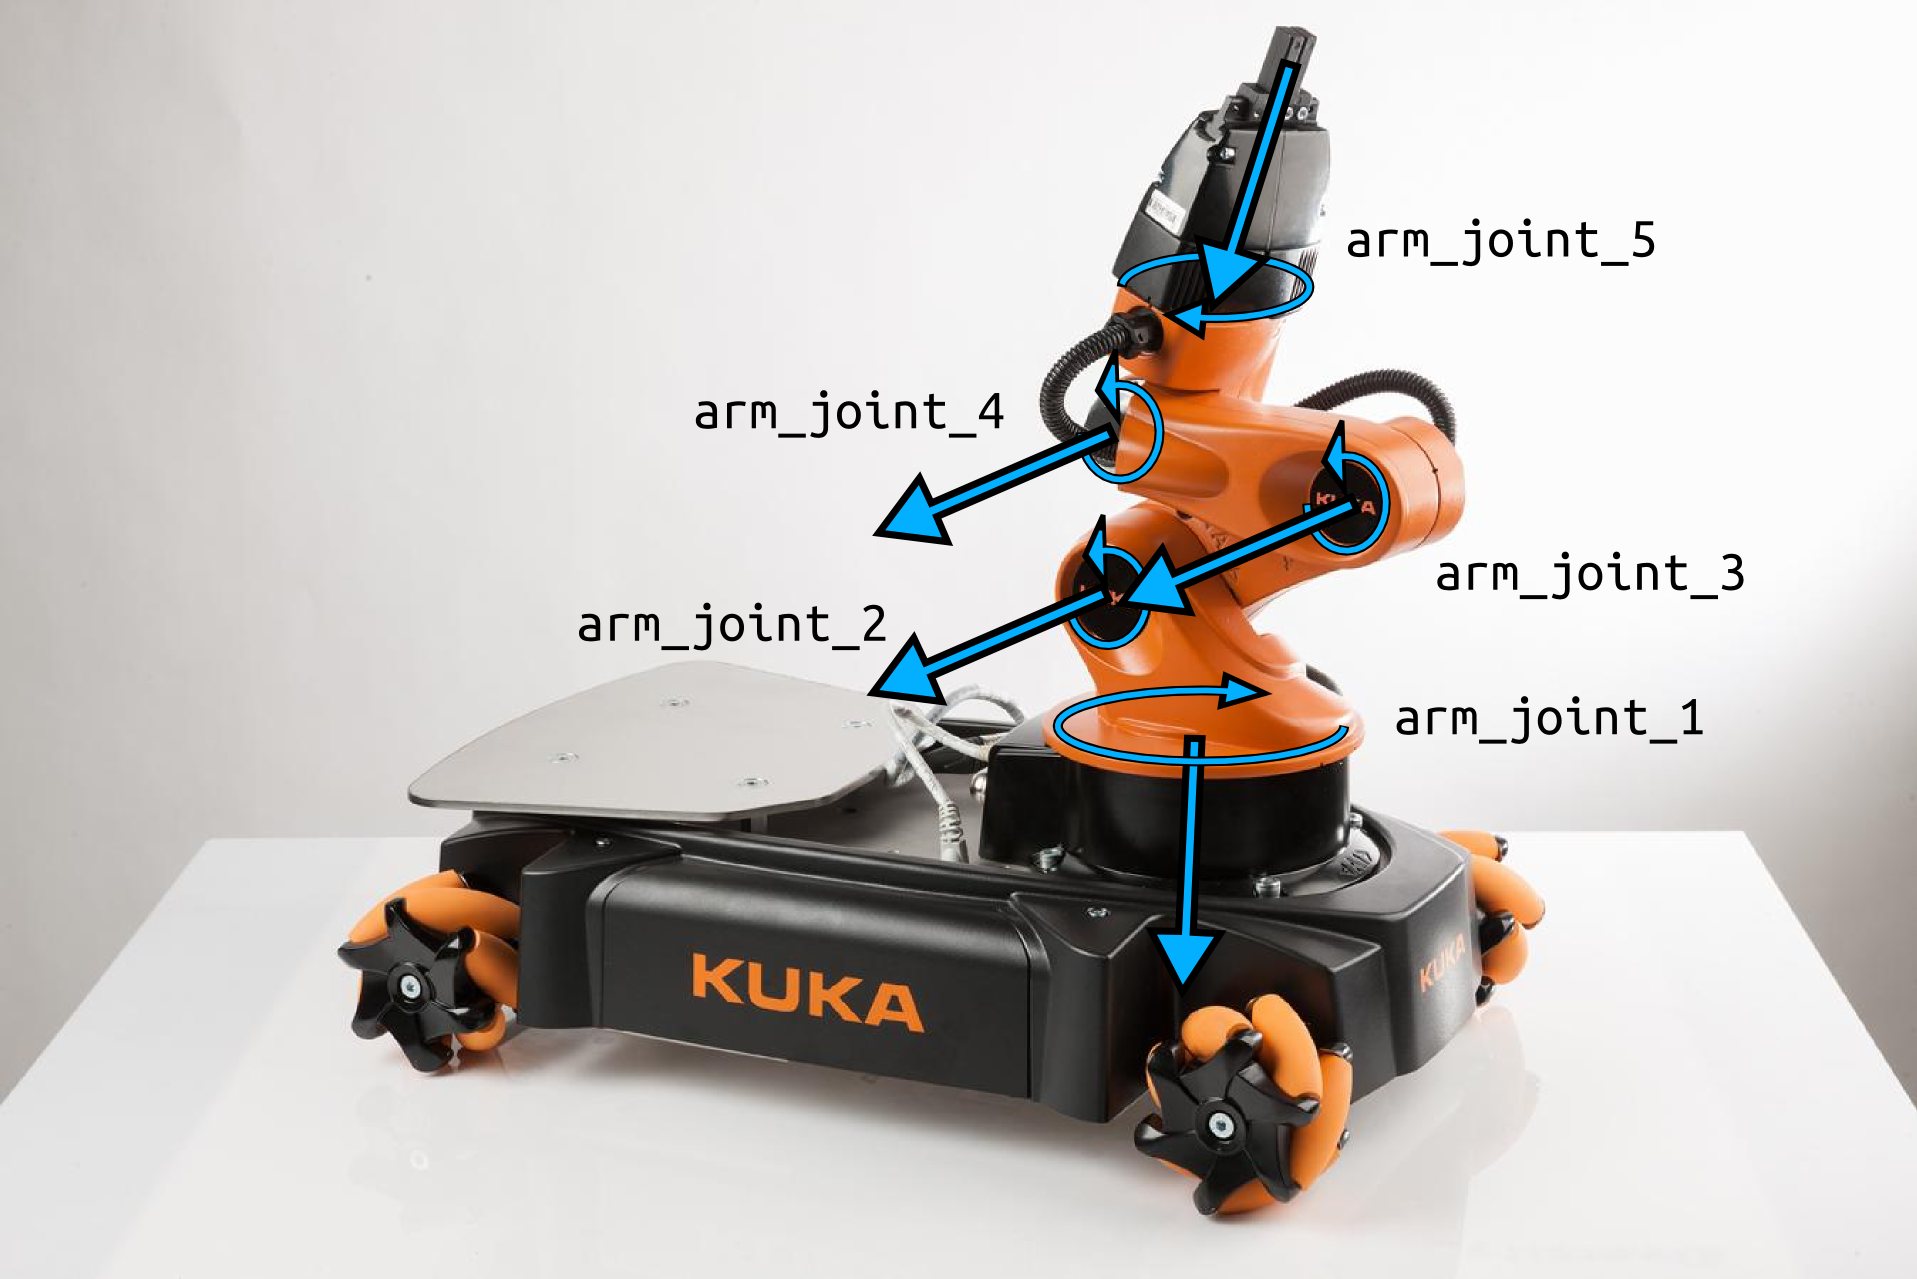
\includegraphics[scale=0.3]{../img/youbot_joints.png} 
	\caption[Articulaciones del brazo robot Youbot]{Articulaciones del brazo del robot Youbot} 
	\label{fig: youbot_joints}
\end{figure}

\subsection{El driver youbot\_oodl}

El driver \textit{youbot\_oodl} es un programa que crea una capa sobre la API de YouBot con el objetivo de poder realizar el control del robot mediante el envío de mensajes a ciertos topics ROS. En el cuadro \ref{tab:topics_youbot} se muestran el nombre del topic y tipo de mensaje que se pueden utilizar para controlar el robot.    

\begin{table}[h]
\footnotesize
\center
\begin{tabular}{|l|l|p{3.5cm}|}
\hline
\multicolumn{3}{|c|}{\textbf{Topics a los que está suscrito el driver youbot\_oodl}}\\
\hline
\textbf{Nombre (espacio /arm\_1)} & \textbf{Tipo} & \textbf{Descripción} \\ 
\hline
/arm\_controller/position\_command & brics\_actuator::JointPositions & Comando con la posición objetivo de las articulaciones \\
/arm\_controller/velocity\_command & brics\_actuator::JointVelocities & Comando con la velocidad objetivo de las articulaciones \\
/gripper\_controller/position\_command & brics\_actuator::JointPositions & Comando con la posición objetivo del gripper \\
\hline
\end{tabular}	
\caption[Topics a los que está suscrito el driver youbot\_oodl]{Topics a los que está suscrito el driver youbot\_oodl de los que lee la posición y velocidad deseadas para cada articulación.}
\label{tab:topics_youbot}	
\end{table}

\subsection{La clase Youbot}

Con un objetivo similar al de la creación de la clase xsens::SensorSubscriberList, la clase Youbot tiene como fin encapsular las comunicaciones de ROS entre el programa \textit{youbot\_controller} y el driver \textit{youbot\_oodl} para que no interfieran en el desarrollo del programa. Esta clase es la encargada de gestionar la publicación de mensajes en los topics de ROS que utiliza el driver \textit{youbot\_oodl} (cuadro \ref{tab:topics_youbot}).\\

Esta clase tiene un funcionamiento muy sencillo. Sólamente es necesario pasarle el \textit{handle} del nodo en el que se declare la clase. Para modificar los valores objetivo de las articulaciones y el \textit{gripper} hay que modificar las variables miembro \textit{joint\_positions[]} y \textit{gripper\_positions[]}. Con el método \textit{PublishMessage()}, se publica en los topics correspondientes los mensajes con las posiciones de las articulaciones. En el siguiente ejemplo se muestra un esquema básico de cómo trabajar con la clase:\\

\lstset{inputencoding=utf8/latin1}
\lstinputlisting[language=C++]{../src/youbot_example.cpp}

La función \textit{PublishMessage()} admite un parámetro de tipo \textit{bool}, que si es \textit{false} (valor por defecto) no publica el mensaje correspondiente a la posición del \textit{gripper}. Si se quisiera controlar el \textit{gripper}, habría que pasar \textit{true} como argumento, pero hay que tener en cuenta que no es posible enviar este mensaje con la misma frecuencia que el mensaje de las articulaciones debido a que el robot no parece poder procesar el mensaje del \textit{gripper} con la suficiente rapidez y se producen comportamientos extraños del robot. De diversas pruebas se ha deducido que la frecuencia más alta de publicación del mensaje del \textit{gripper} para no producir problemas es de 1 Hz.

\section{Otras aplicaciones de visualización y control}

\subsection{Visualizador de la posición del brazo}

El paquete \textit{arm\_visualizer} proporciona una forma de poder visualizar la posición del brazo en el simulador 3D Gazebo. Contiene el nodo \textit{arm\_visualizer}, que básicamente se encarga de leer los topics con los cuaterniones de orientación de tres sensores, con ellos calcula las posiciones y orientaciones de cada eslabón del brazo --brazo, antebrazo y mano-- y publica los correspondientes mensajes de ROS para mover la simulación del brazo en el programa Gazebo. En la sección \textit{Ejecución del simulador del brazo robótico del robot Youbot} del anexo INSTALACIÓN Y PUESTA EN MARCHA DEL SOFTWARE se detalla cómo poner en marcha el visualizador junto con el simulador Gazebo.

\subsection{Controlador de un simulador del brazo robótico del robot Youbot}

En la documentación del robot Youbot existe un paquete de ROS que contiene una simulación del brazo del robot para trabajar en Gazebo y un nodo de ROS --\textit{youbot\_arm\_publisher}-- para realizar su control. Esta simulación está preparada para funcionar tal y como lo hace el robot real; Se puede controlar la posición de las articulaciones con los mismos topics de ROS y los ángulos se corresponden a los del robot real, por lo que se puede usar esta simulación a modo de prueba previa de los programas que se creen para el robot antes de ejecutarlos en el robot real. También puede utilizarse a modo de visualizador de la posición del robot en tiempo real en otro ordenador. En la sección \textit{Instalación del simulador del brazo robótico del YouBot} del anexo INSTALACIÓN Y PUESTA EN MARCHA DEL SOFTWARE se detalla cómo realizar la instalación y puesta en ejecución de esta simulación.

\chapter{PRUEBAS Y RESULTADOS OBTENIDOS}

%%% ******** Capítulo 7 ******** %%%

\chapter{BIBLIOGRAFÍA}


%%% ================ PARTE 2 : ANEXOS ================ %%%

\part{Anexos}

\appendix

\chapter{INSTALACIÓN DEL SOFTWARE}

En el presenta capítulo se describirá como instalar las siguientes herramientas:

\begin{itemize}
\item{ROS Fuerte}
\item{Simulador Gazebo}
\item{Simulador del brazo robótico del Youbot}
\item{Stack de ROS con los programas creados para este proyecto}
\end{itemize}

Se parte de la suposición de que se tiene disponible un ordenador con el sistema operativo Ubuntu 12.04 LTS instalado de forma nativa.

\section{Instalación de ROS Fuerte}

La versión de ROS que se utilizará es ROS Fuerte. Esta elección se debe a que dicha versión es compatible con el simulador Gazebo, con el que posteriormente se realizará la visualización en 3D del modelo. Además es la versión instalada en el PC embebido del robot Youbot.\\

\subsection{Configuración de los repositorios de Ubuntu}

Para comenzar con la instalación se procederá a abrir el Centro de Sofware de Ubuntu y en la barra de menú de dicho programa, se seleccionará en el menú Edit la opción Software Sources. En la pestaña Ubuntu Software se comprobará que están seleccionados los repositorios restricted, universe y multiverse, tal como aparece en la figura \ref{fig: software_sources}.\\

\begin{figure}[h]
	\centering
		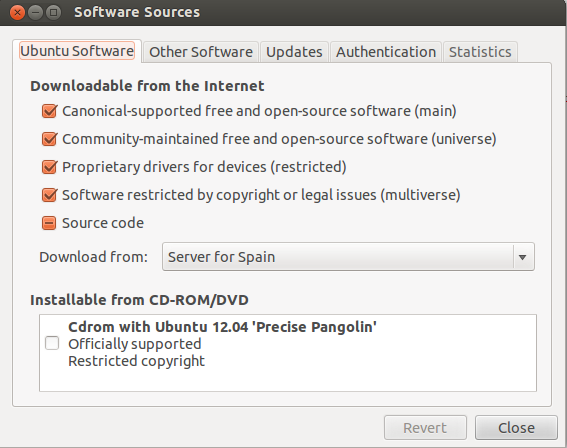
\includegraphics[scale=0.4]{../img/software_sources.png} 
	\caption[Ventana Software Sources]{Ventana Software Sources} 
	\label{fig: software_sources}
\end{figure}

%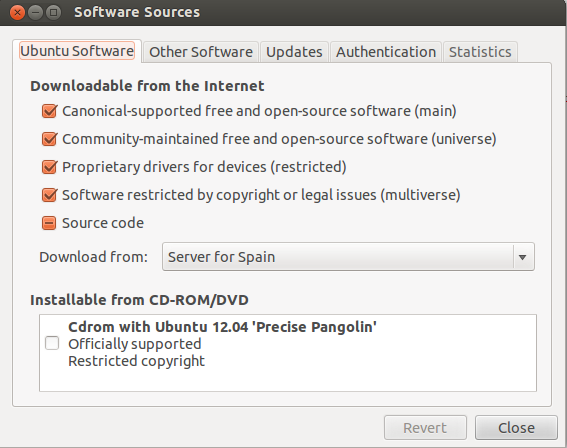
\includegraphics[scale=0.5]{../img/Software sources.png} 

\subsection{Configuración del archivo sources.list}

El archivo sorces.list le dice al gestor de paquetes de Ubuntu de dónde puede obtener cada paquete de ROS. Se abrirá un terminal y se ejecutará el siguiente comando:\\

\begin{verbatim}
$ sudo sh -c 'echo "deb http://packages.ros.org/ros/ubuntu precise main" 
> /etc/apt/sources.list.d/ros-latest.list'
\end{verbatim}

Este comando crea un archivo de texto en la ruta especificada como parámetro, que contiene la dirección de donde descargar los paquetes para la versión específica de ROS que se tenga instalada, en este caso ROS Fuerte.

\subsection{Configuración de la keys}

En el terminal se ejecutará el siguiente comando:

\begin{verbatim}
$ wget http://packages.ros.org/ros.key -O - | sudo apt-key add -
\end{verbatim}

\subsection{Descarga e instalación}

Se actualizará el índice de paquetes de Ubuntu para tener la seguridad de que el servidor de ROS.org está indexado:

\begin{verbatim}
$ sudo apt-get update
\end{verbatim}

A continuación se procederá a descargar e instalar la versión completa de ROS. El el terminal se ejecutará el siguiente comando:

\begin{verbatim}
$ sudo apt-get install ros-fuerte-desktop-full
\end{verbatim}

Esta instalación traerá consigo las herramientas mostradas en la siguiente lista, entre muchas otras:

\begin{itemize}
\item ROS
\item rx (herramientas para interfaz gráfica: rxbag,  rxgraph, rxplot, ...)
\item rviz (herramienta de visualización 3D)
\item librerías genéricas para robots
\item Simuladores 2D/3D (entre ellos Gazebo)
\item Navegación y percepción 2D y 3D
\end{itemize}

\subsection{Configuración del entorno}

Cada vez que se inicie un nuevo terminal es necesario añadir las variables de entorno. Si se quisiera, se puede automatizar dicha tarea ejecutando el comando:

\begin{verbatim}
$ echo “source /opt/ros/fuerte/setup.bash” >> ~/.bashrc
\end{verbatim}

Este comando añade la línea source /opt/ros/fuerte/setup.bash al archivo ~/.bashrc. Este archivo contiene la configuración inicial del terminal, y se ejecuta cada vez que abrimos un nuevo terminal. Posteriormente se ejecutará el archivo anterior para actualizar el terminal. De esta forma reconocerá los nuevos comandos de ROS:

\begin{verbatim}
$ . ~/.bashrc
\end{verbatim}

\section{Instalación del simulador Gazebo}

Si se ha realizado el proceso de instalación de ROS detallado anteriormente, el simulador Gazebo ya vendrá de serie con dicha versión de ROS, y por lo tanto no haría falta seguir los pasos de este apartado. Si se hubiera instalado ROS de otra manera y éste no hubiera venido con el programa Gazebo, se tendría que instalar el programa de forma manual. Para instalar la versión de Gazebo preparada para comunicarse con ROS se ejecutará el siguiente comando:

\begin{verbatim}
$ sudo apt-get install ros-fuerte-simulator-gazebo
\end{verbatim}

\section{Instalación del simulador de brazo robótico del YouBot}

En el robot Youbot ya vienen por defecto los paquetes con los que ejecutar el simulador del brazo robótico con Gazebo. Si se quisiera instalar la simulación en otro ordenador habría que descargarse los paquetes necesarios de la página web de KUKA. Los pasos a seguir son los siguientes:

\begin{enumerate}
\item Descarga de los paquetes con dependencias:

\begin{verbatim}
$ sudo apt-get install ros-fuerte-pr2-controllers
$ sudo apt-get install ros-fuerte-pr2-simulator
\end{verbatim}

\item Instalación desde git de los paquetes con la simulación. Suponemos que se ha creado un \textit{workspace} para trabajar con ROS, y dentro de éste hay una carpeta llamada sandbox:

\begin{verbatim}
$ roscd
$ cd sandbox
$ git clone https://github.com/youbot/youbot-ros-pkg.git
$ git clone https://github.com/ipa320/cob_common.git
\end{verbatim}

\item Compilación de los paquetes

\begin{verbatim}
$ rosmake brics_actuator youbot_description
\end{verbatim}

\end{enumerate}



\section{Instalación del stack youbot-xsens-controller}



\subsection{Instalación desde el CD adjunto al proyecto}

\subsection{Instalación desde git}

\section{PUESTA EN MARCHA DEL SOFTWARE}

\subsection{Iniciación del driver del sensor Xsens}

Para ejecutar el driver \textit{xsens\_node} es necesario iniciar antes el máster de ROS. Para ello en un terminal se ejecutará el siguiente comando:

\begin{verbatim}
$ roscore
\end{verbatim}

A continuación, una vez que los sensores Xsens y el máster Xbus estén conectados al PC, se iniciará el programa driver:

\begin{verbatim}
$ rosrun xsens_driver xsens_node
\end{verbatim}

Si no se ha producido ningún error, ahora el driver estará publicando en ROS los mensajes con los datos leídos del sensor.

\subsection{Iniciación del driver del robot Youbot}

\begin{verbatim}
$ roslaunch youbot_oodl youbot_oodl_driver.launch
\end{verbatim}

\subsection{Ejecución del programa youbot\_controller}

\begin{verbatim}
$ rosrun youbot_controller youbot_controller
\end{verbatim}

\subsection{Ejecución del simulador del brazo robótico del robot Youbot}

Para poner en marcha este programa hace falta haber iniciado primero el driver de los sensores Xsens y el simulador Gazebo. Los pasos a seguir son los siguientes:

\begin{enumerate}
\item Una vez conectados los sensores al PC, en un terminal ejecutamos los siguientes comandos para iniciar el programa \textit{xsens\_node}:

\begin{verbatim}
$ roscore
$ rosrun xsens_driver xsens_node
\end{verbatim}

\item Una vez se compruebe que los sensores están publicando en ROS, se procederá a iniciar Gazebo con el archivo empty\_world.launch:

\begin{verbatim}
$ roslaunch gazebo_world empty_world.launch
\end{verbatim}

\item Se abrirá el GUI de Gazebo, en el que habrá una simulación de un plano (figura \ref{fig: gazebo_empty}). 


\begin{figure}
	\centering
		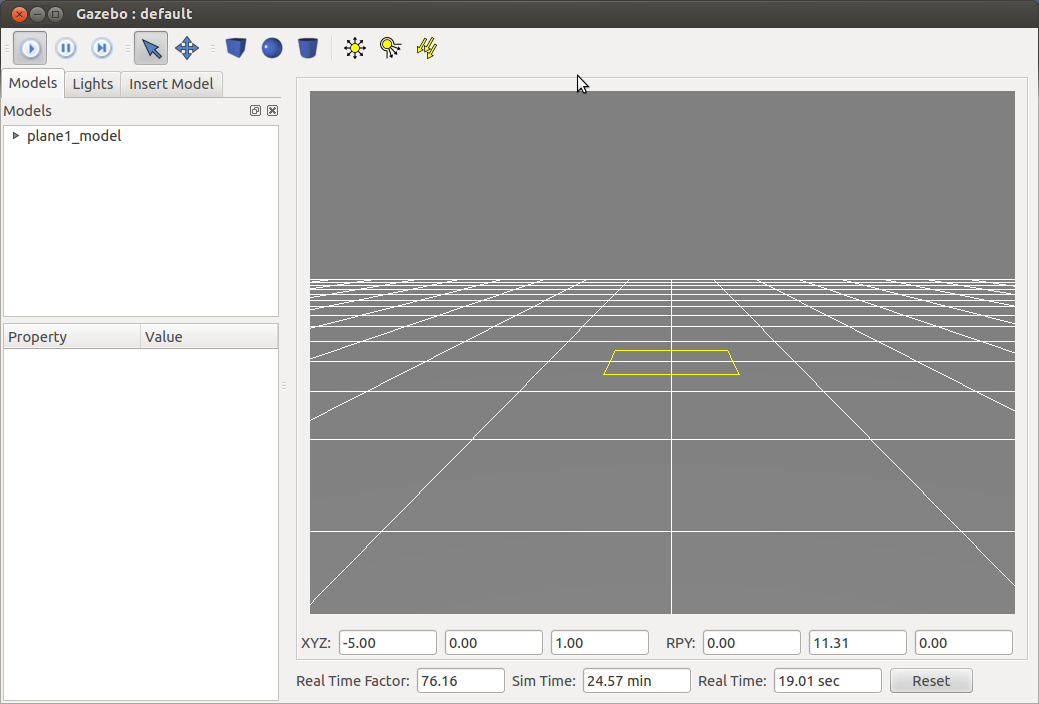
\includegraphics[scale=0.4]{../img/gazebo_empty.png} 
	\caption[Ventana de Gazebo abierta con el archivo empty\_world.launch]{Ventana de Gazebo abierta con el archivo empty\_world.launch} 
	\label{fig: gazebo_empty}
\end{figure}

\item Para la correcta simulación del brazo se tendrá que eliminar el plano de la simulación (figura \ref{fig: gazebo_delete}).

\begin{figure}
	\centering
		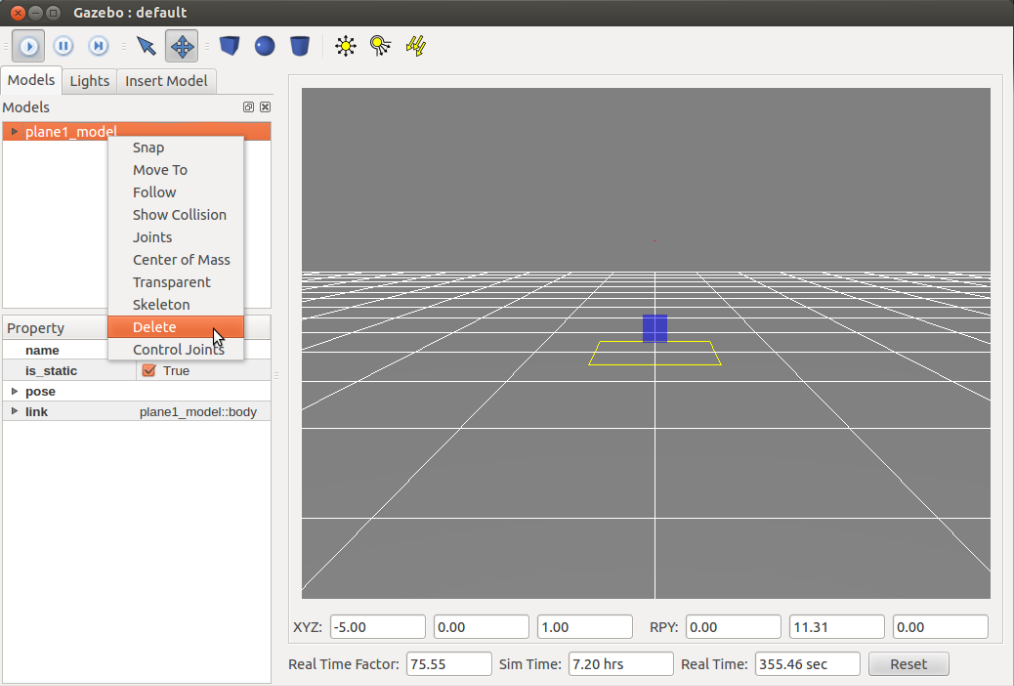
\includegraphics[scale=0.5]{../img/gazebo_delete_2b.png} 
	\caption[Eliminación del plano en la simulación de Gazebo]{Eliminación del plano en la simulación de Gazebo.} 
	\label{fig: gazebo_delete}
\end{figure}

\item También será necesario poner la simulación en pausa, ya que de otra manera se realizará la simulaciñon de la gravedad sobre el brazo y se obtendrán resultados no deseados (figura \ref{fig: gazebo_pause}).

\begin{figure}
	\centering
		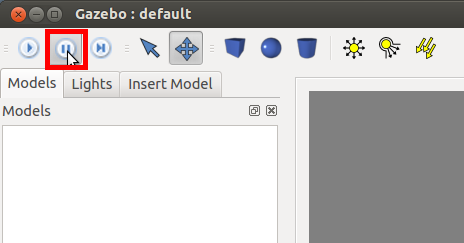
\includegraphics[scale=1.0]{../img/gazebo_pause.png} 
	\caption[Puesta en pausa de la simulación de Gazebo]{Puesta en pausa de la simulación de Gazebo.} 
	\label{fig: gazebo_pause}
\end{figure}

\item A continuación se procederá a ejecutar el programa \textit{arm\_visualizer}, el cuál insertará el brazo en la simulación y se encargará de comunicar a Gazebo las posiciones de cada eslabón del brazo. Para ello en un terminal se ejecutará el siguiente comando:

\begin{verbatim}
$ rosrun arm_visualizer arm_visualizer
\end{verbatim}

\begin{figure}
	\centering
		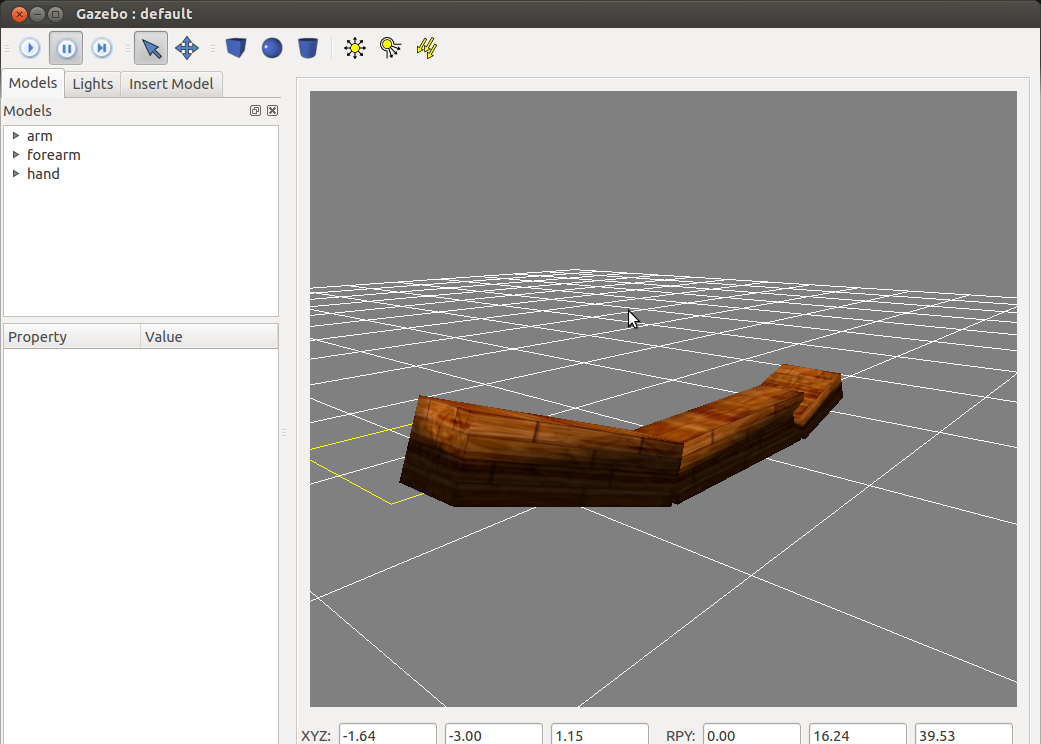
\includegraphics[scale=0.4]{../img/gazebo_arm.png} 
	\caption[Visualización del brazo en Gazebo]{Visualización del brazo en Gazebo.} 
	\label{fig: gazebo_arm}
\end{figure}

\end{enumerate} 

\iffalse

\chapter{CÓDIGO FUENTE}

\section{Driver Xsens}

\subsection{xsens\_node.cpp}
\lstset{inputencoding=utf8/latin1}
\lstinputlisting[language=C++]{../../xsens_driver/src/xsens_node.cpp}
\newpage

\subsection{xsens\_driver.h}
\lstset{inputencoding=utf8/latin1}
\lstinputlisting[language=C++]{../../xsens_driver/include/xsens_driver/xsens_driver.h}
\newpage

\subsection{xsens\_driver.cpp}
\lstset{inputencoding=utf8/latin1}
\lstinputlisting[language=C++]{../../xsens_driver/src/xsens_driver.cpp}
\newpage

\subsection{xsens\_sensor.h}
\lstset{inputencoding=utf8/latin1}
\lstinputlisting[language=C++]{../../xsens_driver/include/xsens_driver/xsens_sensor.h}
\newpage

\subsection{xsens\_sensor.cpp}
\lstset{inputencoding=utf8/latin1}
\lstinputlisting[language=C++]{../../xsens_driver/src/xsens_sensor.cpp}
\newpage

\subsection{xsens\_sensor\_subscriber.h}
\lstset{inputencoding=utf8/latin1}
\lstinputlisting[language=C++]{../../xsens_driver/include/xsens_driver/xsens_sensor_subscriber.h}
\newpage

\subsection{xsens\_sensor\_subscriber.cpp}
\lstset{inputencoding=utf8/latin1}
\lstinputlisting[language=C++]{../../xsens_driver/src/xsens_sensor_subscriber.cpp}
\newpage

\subsection{utils.h}
\lstset{inputencoding=utf8/latin1}
\lstinputlisting[language=C++]{../../xsens_driver/include/xsens_driver/utils.h}
\newpage

\subsection{utils.cpp}
\lstset{inputencoding=utf8/latin1}
\lstinputlisting[language=C++]{../../xsens_driver/src/utils.cpp}
\newpage

\section{Librería dfv}

\subsection{quaternion.h}
\lstset{inputencoding=utf8/latin1}
\lstinputlisting[language=C++]{../../dfv/include/dfv/quaternion.h}
\newpage

\subsection{quaternion.cpp}
\lstset{inputencoding=utf8/latin1}
\lstinputlisting[language=C++]{../../dfv/src/quaternion.cpp}
\newpage

\subsection{vector3.h}
\lstset{inputencoding=utf8/latin1}
\lstinputlisting[language=C++]{../../dfv/include/dfv/vector3.h}
\newpage

\subsection{vector3.cpp}
\lstset{inputencoding=utf8/latin1}
\lstinputlisting[language=C++]{../../dfv/src/vector3.cpp}
\newpage

\subsection{matrix.h}
\lstset{inputencoding=utf8/latin1}
\lstinputlisting[language=C++]{../../dfv/include/dfv/matrix.h}
\newpage

\subsection{matrix.cpp}
\lstset{inputencoding=utf8/latin1}
\lstinputlisting[language=C++]{../../dfv/src/matrix.cpp}
\newpage

\subsection{utils.h}
\lstset{inputencoding=utf8/latin1}
\lstinputlisting[language=C++]{../../dfv/include/dfv/utils.h}
\newpage

\subsection{utils.cpp}
\lstset{inputencoding=utf8/latin1}
\lstinputlisting[language=C++]{../../dfv/src/utils.cpp}
\newpage

\subsection{dfv.h}
\lstset{inputencoding=utf8/latin1}
\lstinputlisting[language=C++]{../../dfv/include/dfv/dfv.h}
\newpage

\section{Youbot controller}

\subsection{youbot\_controller.h}
\lstset{inputencoding=utf8/latin1}
\lstinputlisting[language=C++]{../../youbot_controller/src/youbot_controller.cpp}
\newpage

\subsection{youbot.h}
\lstset{inputencoding=utf8/latin1}
\lstinputlisting[language=C++]{../../youbot_controller/include/youbot_controller/youbot.h}
\newpage

\subsection{youbot.cpp}
\lstset{inputencoding=utf8/latin1}
\lstinputlisting[language=C++]{../../youbot_controller/src/youbot.cpp}
\newpage

\fi

\chapter{SOLUCIÓN DE PROBLEMAS}

\section{Error iniciando Gazebo}

Este error consiste en que al iniciar Gazebo, este no se abre y en la terminal aparecen mensajes parecidos a los que se muestran a continuación:

\footnotesize\begin{spverbatim}
Msg Waiting for master
Msg Connected to gazebo master @ http://localhost:11345
Exception [Master.cc:69] Unable to start server[Address already in use]


terminate called after throwing an instance of 'gazebo::common::Exception'
Aborted (core dumped)
[gazebo-1] process has died [pid 2795, exit code 134, cmd /opt/ros/fuerte/stacks/simulator_gazebo/gazebo/scripts/gazebo /opt/ros/fuerte/stacks/simulator_gazebo/gazebo_worlds/worlds/empty.world __name:=gazebo __log:=/home/daniel/.ros/log/772c2f96-ab75-11e2-a2fc-001de05009b5/gazebo-1.log].
log file: /home/daniel/.ros/log/772c2f96-ab75-11e2-a2fc-001de05009b5/gazebo-1*.log
LightListWidget::OnLightMsg


\end{spverbatim}
\normalsize

Esto es debido a que ya existe un proceso Gazebo ejecutándose en el ordenador pero por alguna razón no ha abierto su interfaz gráfica.

\textbf{Solución: }
Ejecutar comando:
\begin{verbatim}
$ ps ax | grep [g]z
\end{verbatim}

Ver si hay un proceso gzserver

\footnotesize
\begin{spverbatim}
 3118 ?        Sl    12:47
 /opt/ros/fuerte/stacks/simulator_gazebo/gazebo/gazebo/bin/gzserver 
 /opt/ros/fuerte/stacks/simulator_gazebo/gazebo_worlds/worlds/empty.world __name:=gazebo __log:=/home/daniel/.ros/log/8188cc76-ab73-11e2-a4ec-001de05009b5/gazebo-1.log -s /opt/ros/fuerte/stacks/simulator_gazebo/gazebo/lib/libgazebo_ros_paths_plugin.so -s /opt/ros/fuerte/stacks/simulator_gazebo/gazebo/lib/libgazebo_ros_api_plugin.so

\end{spverbatim}
\normalsize

Si lo hay, ejecutar \textit{System Monitor} y matar el proceso \textit{gzserver}.

\section{Al ejecutar el simulador del brazo robótico no se abre la interfaz gráfica de Gazebo}

Es posible que al lanzar Gazebo con el archivo \textit{youbot\_arm\_publisher.launch} no se abra la ventana de Gazebo. Para solucionarlo es necesario abrir dicho archivo y comprobar que sea como el siguiente:

\lstinputlisting[language=xml]{../../doc/src/youbot_arm_publisher.launch}

Este archivo se encuentra en la carpeta \textit{launch/} dentro del paquete\\ 
\textit{youbot-ros-pkg/youbot\_common/youbot\_description}

\section{El driver del Xsens no contacta con los sensores}

\section{Al ejecutar Gazebo con el archivo empty\_world.launch no se abre la GUI}

\begin{verbatim}
[gazebo_gui-2] process has died [pid 28410, exit code 139, cmd /opt/ros/fuerte/stacks/simulator_gazebo/gazebo/scripts/gui __name:=gazebo_gui __log:=/home/daniel/.ros/log/8e1bc56a-ee44-11e2-9ac7-08edb99bab79/gazebo_gui-2.log].
log file: /home/daniel/.ros/log/8e1bc56a-ee44-11e2-9ac7-08edb99bab79/gazebo_gui-2*.log
\end{verbatim}

\part{Presupuesto}

\iffalse

\part{Otros documentos}


\section{Manual del sensor MTi-G}

%\includepdf[pages={-}]{doc/mtig_manual.pdf}

\fi

\end{document}

